\documentclass[11pt]{report}

\usepackage[utf8]{inputenc}
\usepackage[T1]{fontenc}
\usepackage[english]{babel}
\usepackage{geometry}
\geometry{a4paper, margin=1in, headheight=14.5pt} % Adjusted margins with proper headheight
\usepackage{pdfpages}
\usepackage{emptypage} % To ensure blank pages are truly empty
\usepackage{microtype} % Improve justification and reduce overfull hboxes
\usepackage{titlesec} % For custom chapter and section styling
\usepackage{xcolor} % For custom colors
\usepackage[most]{tcolorbox} % For colored boxes
\usepackage{fancyhdr} % For custom headers and footers
\usepackage{tocloft} % For Table of Contents customization
\usepackage{lettrine} % For drop caps
\usepackage{lipsum} % For dummy text if needed
\usepackage{enumitem} % For better list control
\usepackage{caption} % For caption styling
\usepackage{subcaption} % For subfigures
\usepackage{setspace} % For line spacing control
\usepackage{pifont} % For decorative symbols
\usepackage{tikz} % For drawing fancy elements
\usepackage{amssymb} % For mathematical symbols like \checkmark
\usepackage{bookmark} % Better PDF bookmarks
\usepackage{hyperref} % For clickable links in ToC (moved to after other packages)
\usepackage{float}
\usepackage{colortbl} % For colored table cells
\usepackage{array} % For better table column formatting
\usepackage{calc} % For coordinate calculations in TikZ
\usepackage{mdframed} % For framed environments
\usepackage{afterpage} % For operations on the following page
\usepackage{longtable} % For tables that span multiple pages
\usepackage{multicol} % For multi-column layout
\usetikzlibrary{calc}
\tcbuselibrary{skins,breakable}
\usepackage[backend=biber, style=numeric, sorting=none]{biblatex} % Use BibLaTeX
\addbibresource{references.bib} % Specify the BibTeX file
\usepackage{shapepar}
\usepackage{pgfgantt} % For Gantt charts

% \renewcommand*{\bibleftbracket}{<}
% \renewcommand*{\bibrightbracket}{>}

% Define a refined professional color palette
\definecolor{primary}{RGB}{7, 6, 6} % Deep navy blue
\definecolor{secondary}{RGB}{145, 145, 145} % Medium gray
\definecolor{accent}{RGB}{201, 172, 140} % Gold/Bronze accent
\definecolor{background}{RGB}{248, 248, 248} % Light background
\definecolor{bodytext}{RGB}{40, 40, 40} % Near-black for body text

% Set default text color
\color{bodytext}

% Customize chapter style - more elegant
\titleformat{\chapter}[display]
{\normalfont\Large\bfseries\color{primary}}
{\filcenter\color{primary}\MakeUppercase{\chaptertitlename}~\thechapter}
{1em}
{\filcenter\LARGE}[\vspace{0.5em}\centerline{\rule{0.6\textwidth}{1pt}}]
\titlespacing*{\chapter}{0pt}{30pt}{40pt}

% Section styling - more subtle
\titleformat{\section}
{\normalfont\large\bfseries\color{primary}}
{\thesection}{1em}{}
\titlespacing*{\section}{0pt}{3.5ex plus 1ex minus .2ex}{2.3ex plus .2ex}

% Subsection styling
\titleformat{\subsection}
{\normalfont\normalsize\bfseries\color{primary}}
{\thesubsection}{1em}{}

% Set up fancy headers - more elegant
\pagestyle{fancy}
\fancyhf{}
% Remove page number from header
% \fancyhead[R]{\thepage}
\fancyhead[L]{\textit{\leftmark}}
% Add page number to center footer
\fancyfoot[C]{\thepage}
\fancyfoot[R]{\textcolor{secondary}{\small{KORPOR}}}
\renewcommand{\headrulewidth}{0.4pt}
\renewcommand{\footrulewidth}{0.2pt}

% Define a plain pagestyle with page numbers at bottom
\fancypagestyle{plain}{%
  \fancyhf{}%
  \fancyfoot[C]{\thepage}%
  \fancyfoot[R]{\textcolor{secondary}{\small{KORPOR}}}%
  \renewcommand{\headrulewidth}{0pt}%
  \renewcommand{\footrulewidth}{0.2pt}%
}

% Make sure chapter pages show page numbers
\makeatletter
\renewcommand\chapter{\if@openright\cleardoublepage\else\clearpage\fi
                    \thispagestyle{plain}%
                    \global\@topnum\z@
                    \@afterindentfalse
                    \secdef\@chapter\@schapter}
\makeatother

% Enhanced Table of Contents styling
% Title formatting
\renewcommand{\cfttoctitlefont}{\hfill\LARGE\bfseries\color{primary}} 
\renewcommand{\cftaftertoctitle}{\hfill\null\\[1em]\hfill\rule{0.6\textwidth}{1pt}}

% Entry formatting
\renewcommand{\cftchapfont}{\normalfont\bfseries\color{bodytext}} % Chapter font in black
\renewcommand{\cftsecfont}{\normalfont\itshape} % Section font
\renewcommand{\cftsubsecfont}{\normalfont} % Subsection font

% Dot leaders with custom styling
\renewcommand{\cftdot}{$\cdot$} % Better centered dots
\renewcommand{\cftdotsep}{2.0} % Tighter dot spacing
\renewcommand{\cftchapleader}{\color{secondary}\cftdotfill{\cftdotsep}} % Chapter dots
\renewcommand{\cftsecleader}{\color{secondary}\cftdotfill{\cftdotsep}} % Section dots

% Page numbers
\renewcommand{\cftchappagefont}{\normalfont\bfseries\color{bodytext}} % Chapter page number
\renewcommand{\cftsecpagefont}{\normalfont\color{bodytext}} % Section page number

% Spacing for better presentation
\setlength{\cftbeforetoctitleskip}{1em} % Space before title
\setlength{\cftaftertoctitleskip}{2em} % Space after title
\setlength{\cftbeforechapskip}{1em} % Space before chapters
\setlength{\cftbeforesecskip}{0.5em} % Space before sections

% Chapter numbering format
\renewcommand{\cftchappresnum}{\color{primary}} % Color for chapter numbers
\renewcommand{\cftchapaftersnum}{.\hspace{0.8em}} % Add period after number

% Indentation
\setlength{\cftchapindent}{0em} % No indent for chapters
\setlength{\cftsecindent}{1.5em} % Indent for sections
\setlength{\cftsubsecindent}{3em} % Indent for subsections

% Title
\renewcommand{\contentsname}{\color{primary}Table of Contents}

% Improved caption style
\captionsetup{
  font=small,
  labelfont={bf,color=primary},
  margin=10pt,
  format=hang,
  justification=centering,
}

% Lettrine (drop caps) settings - more elegant
\renewcommand{\LettrineFontHook}{\color{primary}\bfseries}
\setcounter{DefaultLines}{3}
\setlength{\DefaultFindent}{0.5em}
\setlength{\DefaultNindent}{0em}
\setlength{\DefaultSlope}{0pt} % Ensure proper alignment

% Define line spacing for main text
\onehalfspacing

% Hyperref settings - more professional
\hypersetup{
    colorlinks=true,
    linkcolor=primary,
    filecolor=primary,
    urlcolor=primary,
    citecolor=primary,
    pdftitle={PFE Rapport},
    pdfauthor={KORPOR},
    % pdfsubject={Final Year Project},
    pdfkeywords={MySQL, Express-Node.js, React, Vite, Blockchain Technology, AI},
    pdfpagemode=UseOutlines,
    pdfstartview=FitH,
    bookmarksopen=true,
    bookmarksnumbered=true,
}

% Define a new environment for important information - more elegant
\newenvironment{important}{%
  \begin{tcolorbox}[
    colback=background,
    colframe=primary,
    arc=1mm, % Slightly rounded corners
    boxrule=0.5pt,
    left=8pt,
    right=8pt,
    top=6pt,
    bottom=6pt,
    width=\textwidth,
    title={\textbf{Important}},
    fonttitle=\color{white}
  ]
}{%
  \end{tcolorbox}
}

% Define a command for first paragraph styling with better alignment
\newcommand{\firstparagraph}[1]{%
  \lettrine[lines=2,findent=0.5em,nindent=0em,loversize=0.05,lraise=0.05]{\textcolor{primary}{#1}}{}%
}

% Define a command for chapter quotes
\newcommand{\chapterquote}[2]{%
  \begin{flushright}
    \begin{minipage}{0.7\textwidth}
      \small\itshape #1
      \begin{flushright}
        \normalfont --- #2
      \end{flushright}
    \end{minipage}
  \end{flushright}
  \vspace{1cm}
}

% Enhanced figure environment with side lines
\newtcolorbox{figureframe}{
  enhanced,
  frame hidden,
  boxrule=0mm,
  sharp corners,
  breakable,
  left=15pt,
  right=0pt,
  top=0pt,
  bottom=0pt,
  toptitle=0pt,
  bottomtitle=0pt,
  colback=white,
}

\let\origfigure\figure
\let\endorigfigure\endfigure

\renewenvironment{figure}[1][htbp]{%
  \origfigure[#1]%
  \begin{figureframe}%
}{%
  \end{figureframe}%
  \endorigfigure%
}

% Styled table environment with decorative side line - same style
\newtcolorbox{tableframe}{
  enhanced,
  frame hidden,
  boxrule=0mm,
  sharp corners,
  breakable,
  left=15pt,
  right=0pt,
  top=0pt,
  bottom=0pt,
  toptitle=0pt,
  bottomtitle=0pt,
  colback=white,
}

\let\origtable\table
\let\endorigtable\endtable
\renewenvironment{table}[1][htbp]{%
  \origtable[#1]%
  \begin{tableframe}%
}{%
  \end{tableframe}%
  \endorigtable%
}

\begin{document}

% Cover Page

\includepdf[pages=1]{cover page.pdf}

% Blank Page after Cover - ensure it's actually blank
% \newpage
% \thispagestyle{empty}
% \null
% \newpage

% % Confidentiality Note
% \vspace*{\fill} % Push to vertical center
% \begin{center}
%     \Large % Increase font size
%     \textbf{Confidentiality Note}\\[1em]
%     Some information in this report has been redacted for confidentiality reasons.
%     Thank you for your understanding.
% \end{center}
% \vfill % Balance vertical space
% \newpage



% Summary and Abstract
% Summary and Abstract on the same page
\thispagestyle{empty} % Remove page style for this page

% Create a more elegant title for Summary
\begin{center}
{\color{primary}\Large\textbf{\MakeUppercase{Summary}}}
\end{center}
\vspace{0.1cm}
\begin{center}
\rule{0.6\textwidth}{1pt}
\end{center}
\vspace{0.5cm}
\addcontentsline{toc}{chapter}{Summary}

\noindent \firstparagraph{T}his work is part of the completion of our Final Year Project at the Higher Institute of Computer Science and Mathematics of Monastir for the academic year 2024-2025, aiming for the National Fundamental License Diploma in Computer Science. Conducted within the company \textbf{\textcolor{primary}{'KZ IT Services'}}, our main objective is the development of a mobile application and a web back-office dedicated to real estate investment named \textbf{\textcolor{primary}{'KORPOR'}}. We used MySQL to manage the databases, Express-Node.js to implement the backend, and React and Vite to implement the frontend. Project management followed the SCRUM Agile methodology, emphasizing agile practices such as sprint planning, sprint management, and regular meetings.

% Keywords in a more professional design
\vspace{0.3cm}
\begin{tcolorbox}[
    colback=background,
    colframe=primary,
    arc=1mm,
    boxrule=0.5pt,
    left=8pt,
    right=8pt,
    top=4pt,
    bottom=4pt,
    width=\textwidth
]
\textbf{Keywords:} MySQL, Express-Node.js, React, Vite.
\end{tcolorbox}

\vspace{1.2cm} % Space between sections

% Horizontal rule to separate sections
\begin{center}
\textcolor{secondary}{\rule{0.7\textwidth}{0.5pt}}
\end{center}

\vspace{1.2cm}

% Create a more elegant title for Abstract
\begin{center}
{\color{primary}\Large\textbf{\MakeUppercase{Abstract}}}
\end{center}
\vspace{0.1cm}
\begin{center}
\rule{0.6\textwidth}{1pt}
\end{center}
\vspace{0.5cm}
\addcontentsline{toc}{chapter}{Abstract}

\noindent \firstparagraph{T}his project is part of our graduation project at the Higher Institute of Computer Science and Mathematics of Monastir for the 2024-2025 academic year, leading to the national diploma of fundamental license in Computer Science.
Carried out within the company \textbf{\textcolor{primary}{"KZ IT Services"}}, our main objective is the development of a mobile application and web back office dedicated to real estate investment called \textbf{\textcolor{primary}{"KORPOR"}}. We used MySQL to manage the databases, Express-Node.js for the backend implementation, and React and Vite for the frontend.
The project management followed the SCRUM Agile methodology, with an emphasis on agile practices such as sprint planning, sprint management, and regular meetings.

% Keywords in a more professional design
\vspace{0.3cm}
\begin{tcolorbox}[
    colback=background,
    colframe=primary,
    arc=1mm,
    boxrule=0.5pt,
    left=8pt,
    right=8pt,
    top=4pt,
    bottom=4pt,
    width=\textwidth
]
\textbf{Keywords:} MySQL, Express-Node.js, React, Vite.
\end{tcolorbox}

% Ensure Summary and Abstract stay on the same page
\nopagebreak 
\cleardoublepage

% Start Arabic page numbering
\pagenumbering{arabic}

% Dedication
\chapter*{\centering Dedication}
\addcontentsline{toc}{chapter}{Dedication}

\begin{center}
{\itshape\large 
To the memory of my beloved father, whose guidance and wisdom continue to light my path. \\
Though no longer with us, your presence remains in every achievement of my life.

\vspace{0.8cm}

To my loving mother, whose strength and endless support shaped who I am today.

\vspace{0.8cm}

To my sister and brother, whose companionship and encouragement \\
have been constant sources of joy and motivation.

\vspace{0.8cm}

To my little Aryouma, whose innocence and love bring happiness to our family every day.

\vspace{0.8cm}

To Mme Nadia, my professors and mentors, who have guided me \\
with knowledge and patience throughout my academic journey.

\vspace{0.8cm}

To my friends, whose encouragement made this journey worthwhile.

\vspace{0.8cm}

\textbf{This work is dedicated to all of you, but especially to you, Father.}
}
\end{center}

\vspace{0.5cm}

% \begin{center}
% 
\includegraphics[width=0.2\textwidth]{images/qr-code-dedication.png}
% \end{center}

% \vspace{1cm}

\begin{flushright}
    \begin{minipage}{0.4\textwidth}
        \centering
        
\includegraphics[width=1\textwidth]{images/Ahmed jaziri signature.png}\\
    \end{minipage}
\end{flushright}

\thispagestyle{empty} 
\thispagestyle{plain}
\cleardoublepage

% Acknowledgement
\chapter*{\centering Acknowledgement}
\addcontentsline{toc}{chapter}{Acknowledgement}
% Add your Acknowledgement content here later 
\thispagestyle{plain}
\cleardoublepage

% Table of Contents with enhanced styling
\thispagestyle{empty}

% Decorative frame for TOC page
\begin{tikzpicture}[remember picture, overlay]
  % Draw a subtle decorative line at top of page
  \draw[color=accent, line width=0.5pt] 
    ([yshift=-1.5cm]current page.north west) -- 
    ([yshift=-1.5cm]current page.north east);
\end{tikzpicture}

\begin{center}
{\color{primary}\LARGE\textbf{\MakeUppercase{Table of Contents}}}

% Decorative element below title
\begin{tikzpicture}
  \draw[color=primary, line width=1pt] (0,0) -- (6,0);
  \draw[color=accent, line width=0.5pt] (1,0.15) -- (5,-0.15);
\end{tikzpicture}
\end{center}

% Hide the default "Contents" heading and remove any default horizontal line
\renewcommand{\contentsname}{}
\renewcommand{\cftaftertoctitle}{}

% This ensures that only the first page of TOC has no page number
\tableofcontents
% Make subsequent pages of TOC have page numbers at bottom
\addtocontents{toc}{\protect\thispagestyle{plain}}

\cleardoublepage

% List of Figures
\thispagestyle{empty}

% Decorative frame for List of Figures page
\begin{tikzpicture}[remember picture, overlay]
  % Draw a subtle decorative line at top of page
  \draw[color=accent, line width=0.5pt] 
    ([yshift=-1.5cm]current page.north west) -- 
    ([yshift=-1.5cm]current page.north east);
  % Draw a matching line at bottom of page  
  \draw[color=accent, line width=0.5pt] 
    ([yshift=0.7cm]current page.south west) -- 
    ([yshift=0.7cm]current page.south east);
\end{tikzpicture}

\begin{center}
{\color{primary}\LARGE\textbf{\MakeUppercase{List of Figures}}}

% Decorative element below title
\begin{tikzpicture}
  \draw[color=primary, line width=1pt] (0,0) -- (6,0);
  \draw[color=accent, line width=0.5pt] (1,0.15) -- (5,-0.15);
\end{tikzpicture}
\end{center}

% Hide the default "List of Figures" heading and remove any default horizontal line
\renewcommand{\listfigurename}{}

\listoffigures
% Make subsequent pages of List of Figures have page numbers at bottom
\addtocontents{lof}{\protect\thispagestyle{plain}}

\cleardoublepage

% General Introduction
\thispagestyle{empty}

\vspace*{\fill}

\begin{center}
\begin{minipage}{1\textwidth}
    \begin{center}
        \large\itshape ``Real estate cannot be lost or stolen, nor can it be carried away. Purchased with common sense, paid for in full, and managed with reasonable care, it is about the safest investment in the world.''\cite{RooseveltRealEstateQuote}
        \vspace{1cm}
        
        \normalfont\textcolor{primary}{— Franklin D. Roosevelt}\\
        \small\textcolor{secondary}{32nd President of the United States}
    \end{center}
\end{minipage}
\end{center}

\vspace*{\fill}

\newpage
\thispagestyle{empty}

\chapter*{\centering General Introduction}
\addcontentsline{toc}{chapter}{General Introduction}
\vspace{-1cm} % Reduce space after title

% \vspace{0.1cm}
% \begin{center}
% % \rule{0.6\textwidth}{1pt}
% \end{center}
% \vspace{0.3cm}

% \vspace{1cm}

\begingroup % Begin group to localize changes
\setlength{\parindent}{0pt} % Remove paragraph indentation
\setlength{\parskip}{0.15em} % Reduce space between paragraphs even more
\footnotesize % Smaller font size to fit on one page

\firstparagraph{I}n today's rapidly evolving financial landscape, traditional investment methods are often burdened by opaque processes, cumbersome bureaucracy, and significant entry barriers. Investors have long struggled with outdated systems that impede transparency, elevate risks, and complicate access to promising opportunities. Such challenges not only limit diversification but also expose users to uncertainties that modern technology can easily overcome.

\noindent \textbf{\textcolor{primary}{Korpor}} was conceived to transform this paradigm by delivering a fully integrated, AI and blockchain-powered mobile investment platform. By harnessing advanced data analytics, machine learning, and cutting-edge blockchain technology, Korpor streamlines every facet of the investment process. The application offers a seamless user onboarding experience, intuitive project listings enriched with AI-driven recommendations, and a secure, automated investment flow that simplifies transactions while ensuring that every operation is recorded immutably on the blockchain. Investors can manage their portfolios effortlessly through a comprehensive dashboard, with real-time notifications, an interactive AI chatbot, and multi-language support delivering a personalized and globally accessible experience.

\noindent \textbf{\textcolor{primary}{Security and trust}} are at the heart of Korpor's design. By employing state-of-the-art encryption, blockchain-based transparency, and strict compliance measures, the platform safeguards sensitive financial data and guarantees that every transaction is executed within a secure and verifiable framework. Continuous monitoring, performance optimization, and the immutable nature of blockchain records further ensure that the application remains resilient, scalable, and resistant to fraud in a dynamic market environment.

\noindent Developed under a flexible Agile framework that combines iterative development with strategic project management best practices, Korpor is designed to rapidly adapt to evolving market trends and user needs. This methodical approach allows for regular feedback, swift enhancements, and the seamless integration of innovative features throughout the development lifecycle.


% Our document is structured as follows:

% \vspace{-0.4cm} % Reduce space before list
\begin{itemize}[leftmargin=1.5em, itemsep=0pt, parsep=0pt, topsep=0.05cm]
\item The first chapter, \textbf{\textcolor{primary}{Project Context}}, delves into the industry challenges and the vision that inspired Korpor's creation.
\item The second chapter, \textbf{\textcolor{primary}{Analysis and Specification of Needs}}, outlines the comprehensive requirements gathering, needs analysis, architectural design, and the selection of cutting-edge tools and technologies.
\item Subsequent chapters document the progressive implementation of core features—from AI-enhanced project recommendations and blockchain-secured transactions to comprehensive portfolio management—each developed through clearly defined sprints encompassing analysis, design, and deployment phases.
\end{itemize}

\vspace{0.05cm}
\noindent Through this structured approach, we demonstrate how Korpor leverages modern technology to reimagine investment management, offering a secure, transparent, and dynamic solution that is set to redefine digital financial engagement.

\endgroup % End group to restore normal settings
\enlargethispage{4cm} % Allow this page to be longer
\cleardoublepage

% Chapter 1: Project Context
\chapter{Project Context}

\section{Introduction}

The aim of this chapter is to present the general framework of the Korpor project, a solution dedicated to real estate investment. In this section, we'll discuss successively:

\begin{itemize}
    \item The presentation of the host organization.
    \item The context and challenges of the real estate sector.
    \item Analysis of existing solutions and identification of their limitations.
    \item Definition of functional and non-functional needs of the mobile application and web back office.
\end{itemize}

\section{Project Context}

This work is part of the end-of-study project for the national diploma of Applied Bachelor's degree in Computer Science from the Higher Institute of Computer Science and Mathematics of Monastir (ISIMM) for the year 2024/2025. I had the opportunity to do my end-of-study internship at the company
``KZ IT Services'', under the supervision of Mr. Khalil Zouari.

\section{Hosting Company}

The purpose of this section is to present the company within which I developed my project, as shown in Figure \ref{fig:hosting-company}.

\begin{figure}[htbp]
    \centering
    
\includegraphics[width=0.2\textwidth]{images/company-logo.png}
    \caption{Hosting Company ``KZ IT Services''}
    \label{fig:hosting-company}
\end{figure}

\subsection{Hosting Company}

\textbf{\textcolor{primary}{KZ IT Service}} is a dynamic software company dedicated to delivering innovative IT solutions tailored to modern business needs. We specialize in designing and developing robust, scalable applications that drive efficiency and digital transformation. Our experienced team leverages cutting-edge technology to create customized software that exceeds client expectations. With a strong commitment to quality and continuous improvement, we build lasting partnerships based on trust and excellence. At ``KZ IT Service'', innovation is at the core of everything we do, empowering our clients to achieve sustainable growth and success.

\section{Preliminary Study}

This preliminary study provides a review of some existing investment and asset management platforms. Further, the next section identifies some key concepts that will lead to further understanding of the domain in question.

\subsection{Existing Solutions Study}

For understanding the present scenario and to clearly demarcate our goals, some renowned investment platform analyses offering similar features, including ``Aseel'' and ``Stake'', are performed \cite{G2CompetitiveAnalysis2024, AsanaCompetitiveAnalysis2024}.

\subsection{Available solutions and analysis}

\subsubsection{The Aseel Platform}

\textbf{\textcolor{primary}{Aseel}} is a portal through which users can invest in different real estate projects with ease. The interface allows the clients to surf various investment opportunities, view the details of the properties, and then make an informed decision. Aseel introduces transparency in the investment process by offering financial data, updates regarding projects, and returns that are estimated. This platform comes with an easy-to-use dashboard through which one tracks their investments and manages their assets without any hassle. The interface of the Aseel Platform is shown in Figure \ref{fig:aseel-platform}.

\newpage

\begin{figure}[htbp]
    \centering
    
\includegraphics[width=0.65\textwidth]{images/Interface-of-the Aseel Platform.png}
    \caption{Interface of ``The Aseel Platform''}
    \label{fig:aseel-platform}
\end{figure}

\begin{center}
    \vspace{0.5em}
    \begin{tikzpicture}
        \draw[primary, line width=1pt] (0,0) -- (0.3\textwidth,0);
        \draw[accent, line width=0.7pt] (0.1\textwidth,-0.07) -- (0.4\textwidth,0.07);
        \fill[primary] (0,0) circle (2pt);
        \fill[accent] (0.3\textwidth,0) circle (2pt);
    \end{tikzpicture}
    \vspace{0.5em}
\end{center}

\subsubsection{The Stake Platform}

\textbf{\textcolor{primary}{Stake}} is an online investment platform that deals with real estate crowdfunding. It provides the opportunity to invest in fractions of property ownership, hence diversifying a portfolio without huge capital. On Stake, there are AI-powered recommendations based on user preferences, seamless payment integration, and a secure environment for investment. Besides, liquidity is guaranteed by enabling exit options for investors who may want to sell their shares in ongoing projects. Figure \ref{fig:stake-platform} illustrates the interface of the Stake Platform.

\newpage
\thispagestyle{empty}
\newpage

\begin{figure}[htbp]
    \centering
    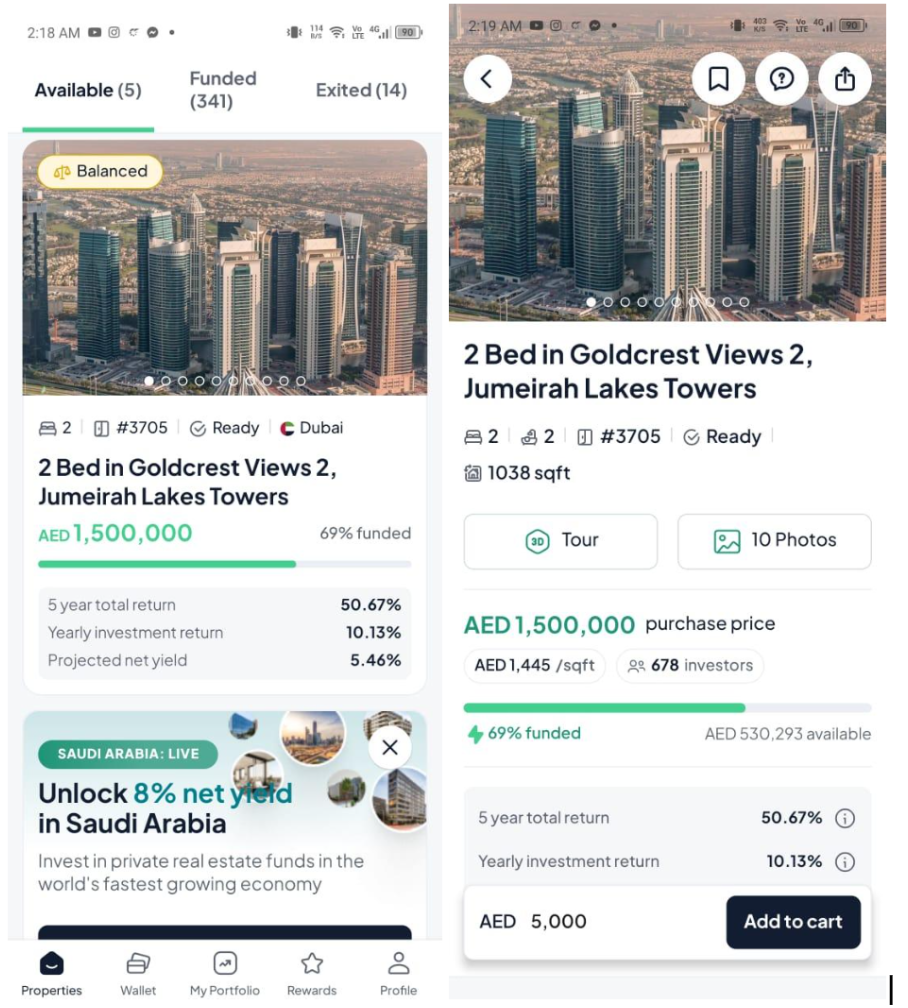
\includegraphics[width=0.65\textwidth]{images/Interface-of-the Stake Platform.png}
    \caption{Interface of ``The Stake Platform''}
    \label{fig:stake-platform}
\end{figure}

\subsection{Comparative and Critical Analysis}

We can summarize all that comes from our analysis based on a number of criteria used for the evaluation of these applications \cite{LyssnaUXAnalysis2024, StrategicManagementInsightCA2024}.

\begin{itemize}
    \item \textbf{Speed (C1)}: The platform should obtain value for the user as fast as possible and effectively, anticipating their proliferating expectations.
    \item \textbf{Costs (C2)}: With minimum software development costs, it is important to keep the pricing predictable and acceptable.
    \item \textbf{Quality (C3)}: Since the market expects quality, any kind of error might affect brand reputation. Improvement of the platform should be regular.
    \item \textbf{Reliability (C4)}: Since modern-day investment platforms need to make sure of minimum downtime and maximum availability of services, this factor is critical.
    \item \textbf{Security (C5)}: Such an investment platform enforces access rights, roles, and contribution rights through a powerful security system.
    \item \textbf{Performance (C6)}: Crucial features include AI-powered recommendations going through seamlessly, easy transaction tracking, and investment monitoring.
    \item \textbf{Stability (C7)}: The platform should have a proven track record, regular updates, and a large user base to ensure its longevity.
    \item \textbf{Resilience (C8)}: In order to prevent data loss and guarantee a smooth experience for investors, it must be able to restore lost functionalities should issues occur.
    \item \textbf{User Experience (C9)}: The interface should be intuitive and user-friendly, hence allowing investors to move with ease through it, thus making wiser decisions.
\end{itemize}

Table \ref{tab:evaluation} presents the evaluation of the existing solutions based on these criteria:

\begin{table}[htbp]
    \centering
    \caption{Evaluation Table}
    \label{tab:evaluation}
    \renewcommand{\arraystretch}{1.3}
    \begin{tabular}{|>{\columncolor{background}}c|*{9}{>{\centering\arraybackslash}p{0.7cm}|}}
        \hline
        \rowcolor{primary!15}
        \textcolor{primary}{\textbf{Solution}} & 
        \textcolor{primary}{\textbf{C1}} & 
        \textcolor{primary}{\textbf{C2}} & 
        \textcolor{primary}{\textbf{C3}} & 
        \textcolor{primary}{\textbf{C4}} & 
        \textcolor{primary}{\textbf{C5}} & 
        \textcolor{primary}{\textbf{C6}} & 
        \textcolor{primary}{\textbf{C7}} & 
        \textcolor{primary}{\textbf{C8}} & 
        \textcolor{primary}{\textbf{C9}} \\
        \hline
        \textbf{Stake} & \textcolor{primary}{\checkmark} & \textcolor{primary}{\checkmark} & \textcolor{primary}{\checkmark} & \textcolor{primary}{\checkmark} & \textcolor{primary}{\checkmark} & $\times$ & \textcolor{primary}{\checkmark} & \textcolor{primary}{\checkmark} & \textcolor{primary}{\checkmark} \\
        \hline
        \rowcolor{background!50}
        \textbf{Aseel} & \textcolor{primary}{\checkmark} & \textcolor{primary}{\checkmark} & \textcolor{primary}{\checkmark} & $\times$ & \textcolor{primary}{\checkmark} & $\times$ & \textcolor{primary}{\checkmark} & $\times$ & \textcolor{primary}{\checkmark} \\
        \hline
    \end{tabular}
\end{table}

\subsection{Proposed Solution}

Having studied the already working platforms for investments, we found strengths and weaknesses that could define what was required from the project. Our proposed solution will look at:

\begin{itemize}
    \item Developing an efficient mobile application for investment management.
    \item Increasing the level of users' engagement with recommendations using the power of AI \cite{MobileRealityAIRealEstate2024, HouseCanaryAIInvestors2024, SmilkovTensorFlowJS2019}.
    \item Ensuring responsive and user-friendly interaction with the interface.
    \item Gaining the trust of investors by ensuring transparency and security in the investing platform.
    \item Enhancing the security of data and following all the financial regulations.
\end{itemize}

The \textbf{\textcolor{primary}{Korpor}} platform will be offering the following features:

\begin{itemize}
    \item A directory of investment opportunities with deep financial insights into those opportunities.
    \item AI-driven recommendations of investments as per users' preferences \cite{LinkedInAIFinTech2024}.
    \item Smooth funding and payout mechanisms.
    \item Real-time portfolio performance tracking on a single screen/dashboard.
    \item Forum for interactive discussions on strategy and market trends among its users.
    \item Referral and Rewards System: An engaging system for rewarding users via referral.
\end{itemize}

\section{Development methodology}

The completion of the project on its delivery date is the main problem of every software development team. One of the most common problems encountered in the production of software is insufficient technical specifications, poor time management in the face of the use of emerging technology, and sudden changes in needs. In order to avoid these critical issues, we follow an agile methodology for project management, using tools like Git \cite{GitWebsite} for version control and GitHub \cite{GithubWebsite} for collaborative development.

\subsection{SCRUM}

\textbf{\textcolor{primary}{Scrum}} is an agile development approach that is used to create software using incremental and iterative methods. Scrum is a quick, flexible, and efficient agile methodology that is intended to provide value to the client at every stage of the project's development \cite{ScrumGuide2020}. Scrum is founded on empiricism and lean thinking, employing an iterative, incremental approach guided by the three pillars of transparency, inspection, and adaptation \cite{AtlassianScrumPillars, ScrumGuide2020}. Scrum's main goal is to meet customer needs by fostering an atmosphere of open communication, group accountability, and constant improvement, underpinned by the Scrum values of Commitment, Focus, Openness, Respect, and Courage \cite{ScrumGuide2020}. The development process begins with a broad concept of what must be constructed, developing a list of features that the product owner desires, and arranging them according to priority (product backlog).

\subsection{Agile Scrum roles and responsibilities}

\subsubsection{The Product Owner}

Understands the customer and business requirements, then creates and manages the product backlog based on those requirements.

\textbf{Responsibilities:}
\begin{itemize}
    \item Managing the scrum backlog
    \item Release management
    \item Stakeholder management
\end{itemize}

\subsubsection{Developers}

In Scrum, the term developer or team member refers to anyone who plays a role in the development and support of the product and can include researchers, architects, designers, programmers, etc.

\textbf{Responsibilities:}
\begin{itemize}
    \item Delivering the work through the sprint
    \item To ensure transparency during the sprint, they meet daily at the daily scrum
\end{itemize}

\subsubsection{Scrum Master}

The role responsible for gluing everything together and ensuring that scrum is being done well. In practical terms, that means they help the product owner define value, the development team deliver the value, and the scrum team get better.

The Scrum Master focuses on:
\begin{itemize}
    \item Transparency
    \item Empiricism
    \item Self-organization
    \item The Scrum events
\end{itemize}

\subsection{The Scrum Events}

The Scrum events are key elements of the Scrum Framework. They provide regular opportunities for enacting the Scrum pillars of Inspection, Adaptation and Transparency \cite{ScrumGuide2020}. In addition, they help teams keep aligned with the Sprint and Product Goals, improve Developer productivity, and remove impediments and reduce the need to schedule too many additional meetings.

\begin{itemize}
    \item \textbf{Sprint}: All work in Scrum is done in a series of short projects called Sprints. This enables rapid feedback loops.
    
    \item \textbf{Sprint Planning}: The Sprint starts with a planning session in which the Developers plan the work they intend to do in the Sprint. This plan creates a shared understanding and alignment among the team.
    
    \item \textbf{Daily Scrum}: The Developers meet daily to inspect their progress toward the Sprint Goal, discuss any challenges they've run into, and tweak their plan for the next day as needed.
    
    \item \textbf{Sprint Review}: At the end of the Sprint, the Scrum Team meets with stakeholders to show what they have accomplished and get feedback.
    
    \item \textbf{Sprint Retrospective}: Finally, the Scrum Team gets together to discuss how the Sprint went and if there are things they could do differently and improve in the next Sprint.
\end{itemize}

\section{Conclusion}

In conclusion of this chapter, it is clear that planning and methodology are essential pillars to ensure the success of the project. By fully understanding the project framework, including the host organization's expectations and the challenges ahead, the team is better prepared to meet the challenges ahead.

This chapter lays the solid foundation on which the entire project will be built, providing a valuable guide for the next steps. The next chapter will allow us to analyze and specify the needs developed in our project. 
\cleardoublepage

% Chapter 2: Analysis and Specification
\chapter{Requirements Specification and Analysis}

\section*{Introduction}

  In this chapter, we will present the analysis and specification of Requirements. We start by presenting the specification of the requirements, illustrating them using global use case diagram. Then we will present our project architecture and our working environment, and finally the product backlog and release planning, and we will close our chapter with a conclusion.

\section{Requirements Specification}

In this section, we will define the actors of our application and the functional and non-functional Requirements that our application aims to fulfill.

\subsection{Identifying Actors}

We define actors as a shorthand for the roles played by entities outside the system that interact directly with them \cite{CockburnUML2002, CockburnWritingEffectiveUseCases2000}. In our system, we identify four types of actors:

\begin{itemize}
    \item \textbf{\textcolor{primary}{Super Admin}}: Responsible for the global configuration of the platform, they have extended privileges to manage administrators, oversee security, and ensure compliance. They can also configure advanced features and control all system resources.
    
    \item \textbf{\textcolor{primary}{Admin}}: In charge of the day-to-day management of the platform, they can add, modify, or delete listings, supervise agency and user profiles, and ensure smooth operations. They are also responsible for monitoring and assisting other actors.
    
    \item \textbf{\textcolor{primary}{Real Estate Agent}}: Dedicated to creating and updating real estate listings, they manage property information, handle investor requests, and finalize transactions related to sales or rentals. They can also coordinate property visits and propose tailored offers.
    
    \item \textbf{\textcolor{primary}{Investor}}: A user who wishes to browse and finance real estate projects. They have access to all available offers, can make investments in a few simple steps, and monitor the evolution of their portfolio. They also benefit from personalized insights to optimize their investments.
    
    \item \textbf{\textcolor{primary}{System}}: The entity that automatically manages all basic functionalities, such as authentication, notification generation, transaction validation, and adherence to security protocols. It ensures the coherence and reliability of the application at all times.
\end{itemize} 

\subsection{Functional Requirements}

\addtocontents{toc}{\protect\newpage}
After several meetings with our client, the various functional requirements of our application are illustrated as follows:

\subsubsection{For the Super Admin (Korpor)}
\begin{itemize}
    \item \textbf{Authenticate}: The super admin enters their credentials to access the advanced management console.
    \item \textbf{Log Out}: After viewing or updating global settings, they can securely log out.
    \item \textbf{Manage Admin Accounts}: Create, enable/disable, or modify admin profiles associated with different real estate companies.
    \item \textbf{Monitor Security \& Compliance}: Oversee transactions, data integrity, and regulatory adherence using specialized reporting and audit tools.
    \item \textbf{Configure Platform Features}: Define key parameters (payment methods, AI/blockchain integrations, etc.) and roll out feature updates.
    \item \textbf{View Global Reports}: Generate and analyze consolidated metrics (financials, user activity, transactions) for overall performance insights.
    \item \textbf{Moderate Content}: Review and remove any inappropriate or erroneous property listings or user-generated data.
\end{itemize} 

\subsubsection{For the Admin (Real Estate Company)}
\begin{itemize}
    \item \textbf{Authenticate}: The admin logs in with valid credentials to manage daily operations.
    \item \textbf{Log Out}: They can end their session to maintain account security.
    \item \textbf{Manage Real Estate Listings}: Add, update, or delete property listings visible to investors.
    \item \textbf{Oversee Real Estate Agents}: Create and manage agent accounts, assign properties, and monitor performance and commissions.
    \item \textbf{Track Transactions \& Commissions}: Review incoming payments, calculate commissions owed to agents, and track the history of completed deals.
    \item \textbf{Address Investor Inquiries}: Respond to questions or concerns from investors, ensuring a smooth user experience.
    \item \textbf{Access Agency Dashboard}: View comprehensive statistics on properties, sales, rentals, and market trends.
\end{itemize}

\subsubsection{For the Real Estate Agent}
\begin{itemize}
    \item \textbf{Authenticate}: The agent logs in to manage assigned properties and interact with potential investors.
    \item \textbf{Log Out}: Securely exit the account after completing tasks.
    \item \textbf{Manage Assigned Properties}: Create new listings, update property details, set prices, and upload images.
    \item \textbf{Handle Investment Requests}: Review purchase or rental offers, negotiate terms, and initiate contract finalization.
    \item \textbf{Contribute to AI Estimates}: Provide or refine data to improve AI-driven pricing and market analysis.
    \item \textbf{Maintain Client Relationships}: Communicate with investors, schedule property visits, and follow up on inquiries.
    \item \textbf{View Commissions}: Track earnings based on successful sales or rentals.
\end{itemize}

\subsubsection{For the Investor (Mobile App User)}
\begin{itemize}
    \item \textbf{Create an account \& authenticate}: Register to gain access to the platform's core features.
    \item \textbf{Log Out}: End the session to protect personal and financial data.
    \item \textbf{Browse Listings \& Invest}: Explore available properties, filter according to preferences, and commit to an investment in a few steps.
    \item \textbf{Track Portfolio}: Monitor owned assets, property status, and receive real-time updates on performance.
    \item \textbf{Make Payments}: Use integrated payment methods (credit cards, digital wallets, etc.) to complete transactions.
    \item \textbf{Access AI Recommendations}: View data-driven insights and return-on-investment estimates generated by the system.
    \item \textbf{Manage Withdrawals \& Earnings}: Withdraw profits, monitor rental income, or exit investments under the right conditions.
\end{itemize}

\subsubsection{For the System}
\begin{itemize}
    \item \textbf{Automate Authentication}: Validate credentials, manage sessions, and maintain user roles and permissions.
    \item \textbf{Generate Notifications}: Send real-time alerts (e.g., new listings, completed transactions, commission updates) to relevant users.
    \item \textbf{Ensure Compliance \& Security}: Leverage blockchain for data integrity, verify payments, and detect anomalies or fraudulent activities.
    \item \textbf{Coordinate AI Insights}: Aggregate and analyze real estate data to produce market predictions and price recommendations.
    \item \textbf{Maintain Transaction Consistency}: Update dashboards, user balances, and property statuses automatically upon each operation.
    \item \textbf{Optimize Performance}: Monitor server load, scale resources, and ensure a smooth, responsive application experience.
\end{itemize} 

\subsection{Non-functional Requirements}

In order to ensure the proper functioning of the decision-making system and to avoid any kind of anomaly, the implemented solution must meet a set of non-functional needs such as:

\begin{itemize}
    \item \textbf{Maintainability}: The system must be designed for simplicity so that tasks, updates, and bug fixes can be executed with minimal complexity \cite{DevOpsFoundation2023, FowlerRefactoring2018}.
    
    \item \textbf{Evolution}: Platform administration must remain attentive to user needs and feedback, continuously enhancing the services offered while preserving the application's utility and efficiency \cite{PoppendieckLean2012, KnibergLeanStartup2013}.
    
    \item \textbf{Security}: Robust security measures are essential. The platform must enforce strong authentication protocols, access privileges, and comprehensive data encryption (both at rest and in transit) \cite{ClerkAuthenticationDocs, OWASPSecurityPrinciples2021}. The integration of blockchain technology further ensures the immutability and integrity of sensitive information \cite{WangBlockchainRealEstate2023, McKinseyBlockchainRE2023}.
    
    \item \textbf{Efficiency}: The application must be effective in all circumstances, delivering prompt and reliable functionality regardless of external conditions \cite{KimDevOpsMethods2018, BassArchitecture2021}.
    
    \item \textbf{Performance}: The system must operate optimally across diverse environments. It should consistently provide a responsive and reliable experience, even under high transaction volumes or varying network conditions \cite{DockerArchitecture2023, ForsgreniDevOpsMetrics2023}.
\end{itemize} 

\section{Requirements Analysis}

In this section, we'll outline the various features that our app should offer, using a general use case diagram \cite{CockburnUML2002}.

\subsection{General use case diagram}

Below, we present the various actors of the application and the actions they are authorized to perform.
The overall diagram is illustrated in Figure \ref{fig:use-case-diagram}:

\begin{figure}[htbp]
    \centering
    % Replace with actual image file once available
    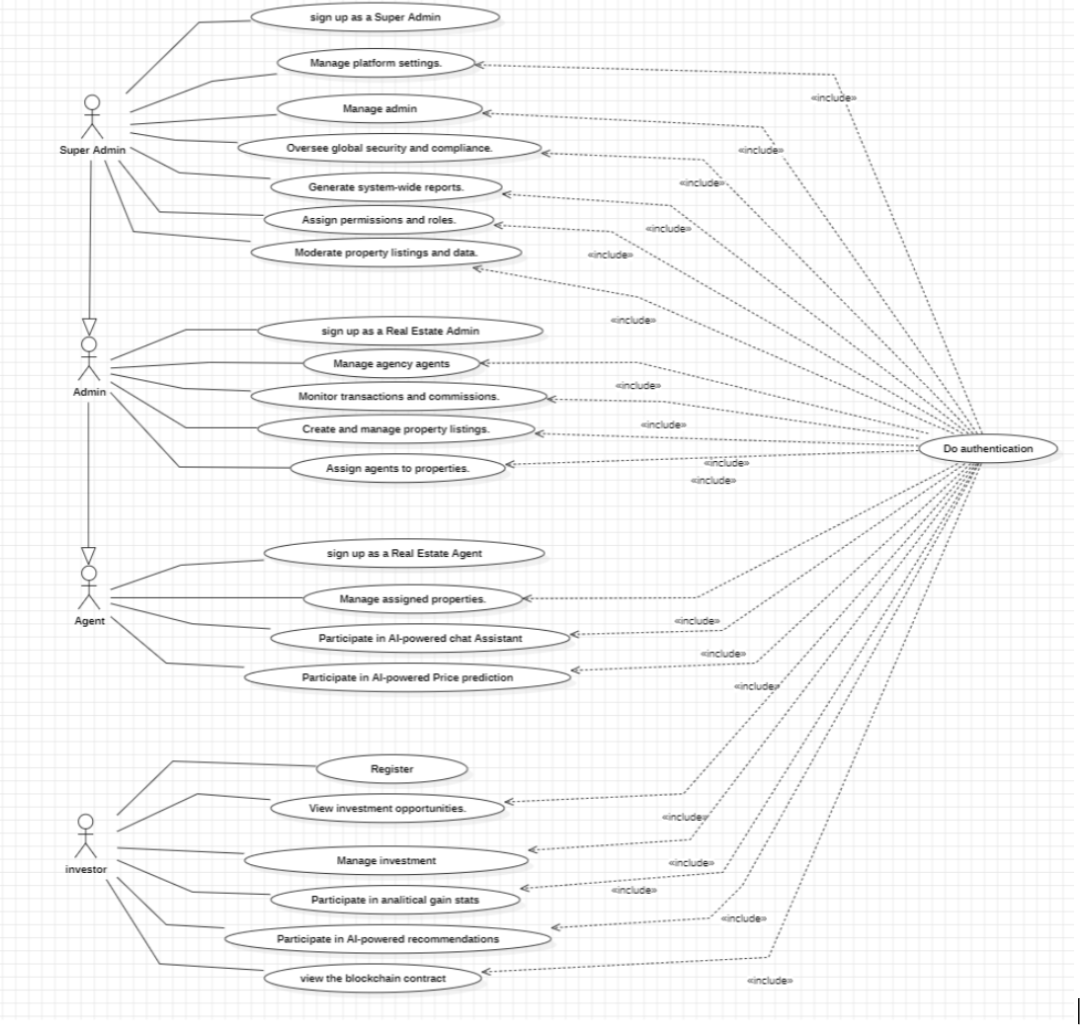
\includegraphics[width=0.6\textwidth]{images/diagram de case d utilisation general.png}
    \caption{General use case diagram}
    \label{fig:use-case-diagram}
\end{figure}
\newpage
\section{Software architecture}

Before starting the design and development of any computerized system, it is essential to prepare the architecture.

\subsection{Physical architecture}

 The physical architecture of Korpor leverages modern, scalable technologies to deliver a seamless investment platform. The frontend is built with Expo, React, and TypeScript using Vite \cite{ViteJSWebsite} for rapid development and Tanstack for robust state management and data visualization, while Storybook supports isolated UI component development \cite{StorybookDocs2022}. The backend relies on Express.js \cite{ExpressJSWebsite} with user authentication managed by Clerk \cite{ClerkAuthenticationDocs}, containerization via Docker \cite{DockerArchitecture2023}, and MySQL \cite{MySQLWebsite} for data storage hosted on Microsoft Azure \cite{AzureCloudServices2024}. Integrated AI modules provide personalized insights \cite{JohnsonAIPropertyValuation2024}, and blockchain technology ensures transactional security and data immutability \cite{WangBlockchainRealEstate2023, McKinseyBlockchainRE2023}. This setup is further supported by GitHub \cite{GithubWebsite} for version control, Postman \cite{PostmanWebsite} for API testing, and end-to-end testing tools like Maestro and Playwright \cite{PlaywrightDocs2023}, with architectural designs and documentation maintained using StarUML \cite{StarUMLWebsite} and Overleaf.

\begin{figure}[htbp]
    \centering
    % Replace with actual image file once available
    % \includegraphics[width=0.85\textwidth]{images/physical_architecture.png}
    \caption{Deployment diagram}
    \label{fig:physical-architecture}
\end{figure}

\subsection{Logical architecture}

To better manage code organization and ensure maintainability, we've designed our application based on the MVC (Model-View-Controller) \cite{SunardiMVC2019, GammaPatterns1994} architectural pattern:

\begin{itemize}
    \item \textbf{Model}: Represents application data and business logic.
    \item \textbf{View}: Presents data to users through interfaces.
    \item \textbf{Controller}: Processes incoming requests, performs operations using Models, and returns appropriate Views.
\end{itemize}

Architecture Components:
\begin{itemize}
    \item \textbf{Model:} The data layer interacts with the backend through ORM or query-based operations, ensuring efficient data retrieval and persistence.
    
    \item \textbf{Controller:} The Express.js backend acts as the intermediary between the database and the frontend, handling user requests, business logic, and data validation. It processes API calls from the frontend and interacts with services such as Clerk for authentication, AI modules for predictive analytics, and blockchain integration for secure transactions.
    
    \item \textbf{View:} The frontend is built with React, TypeScript, and TanStack tools, ensuring a responsive and interactive UI. The frontend communicates with the backend via API requests, displaying dynamic content and allowing seamless user interaction.
\end{itemize}

The logical architecture is illustrated in Figure \ref{fig:logical-architecture}.

\begin{figure}[htbp]
    \centering
    % Replace with actual image file once available
    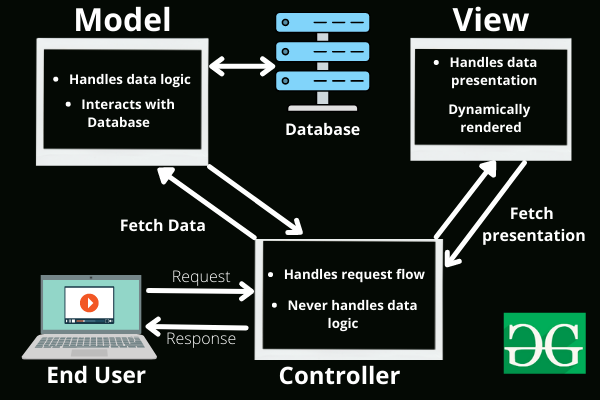
\includegraphics[width=0.9\textwidth]{images/logique.png}
    \caption{Logical architecture}
    \label{fig:logical-architecture}
\end{figure}

Request Flow:
\begin{enumerate}
    \item A user action (e.g., viewing property listings) triggers a request in the frontend.
    \item The request is sent to the backend via an API call.
    \item The Express.js controller processes the request, interacting with the database and other services.
    \item Data is retrieved, processed, and returned as a response.
    \item The frontend updates the UI dynamically based on the received data.
\end{enumerate}

This structured approach ensures a scalable, secure, and high-performance system, optimizing Korpor's real estate investment and management operations \cite{KimDevOpsMethods2018}.

\section{Work Environment}

In this part, we will talk about our work environment, focusing on different aspects:
our material environment, the techniques we used in the realization of our project as well as the tools we used in our report, the product backlog and sprint planning, and finally, we will conclude this section \cite{BeckXP2004, MartinCleanArchitecture2017}.

\subsection{Physical environment}

The work was carried out by a laptop computer that is equipped with these detailed features presented in Table \ref{tab:physical-env} below:

\begin{table}[htbp]
    \centering
    \begin{tabular}{|l|l|}
        \hline
        \textbf{Computer Name} & MSI \\
        \hline
        \textbf{Processor} & i5 10th gen \\
        \hline
        \textbf{Hard disk} & 512 Go SSD \\
        \hline
        \textbf{RAM} & 24.0 Go \\
        \hline
        \textbf{Operating system} & Windows 11 Pro \\
        \hline
    \end{tabular}
    \caption{Physical environment}
    \label{tab:physical-env}
\end{table}

\subsection{Used technologies}

% Define a command for technology icons to make it easier to adjust if needed
\newcommand{\techicon}[1]{%
  \includegraphics[height=1em]{images/icons/#1.png}%
}

\subsubsection*{\protect\techicon{expo} Expo}

Expo is an open-source platform for making universal native apps for Android, iOS, and the web with JavaScript and React.

\subsubsection*{\protect\techicon{typescript} TypeScript}
                                                                
TypeScript (abbreviated as TS) is a free and open-source high-level programming language developed by Microsoft that adds static typing with optional type annotations to JavaScript \cite{TypeScriptDocs2023}. It is designed for the development of large applications and transpiles to JavaScript.

\subsubsection*{\protect\techicon{tanstack} Tanstack}
                                                                      
High-quality open-source software for web developers \cite{TanstackWebsite}. Headless, type-safe, \& powerful utilities for Web Applications, Routing, State Management, Data Visualization, Datagrids/Tables, and more.

\subsubsection*{\protect\techicon{clerk} Clerk}
                                                                        
Clerk \cite{ClerkAuthenticationDocs} is a complete suite of embeddable UIs, flexible APIs, and admin dashboards to authenticate and manage your users.

\subsubsection*{\protect\techicon{maestro} Maestro}
                                                                        
Maestro \cite{MaestroDocs2022} is the simplest, most powerful, and most trusted end-to-end testing platform for mobile and web apps.

\subsubsection*{\protect\techicon{azure} Google cloud platform}

Google cloud platform, or just GCP, is the cloud computing platform developed by Google. It has management, access and development of applications and services to individuals, companies, and governments through its global infrastructure.

\subsubsection*{\protect\techicon{github} GitHub}

GitHub \cite{GithubWebsite} is a cloud-based service that helps developers store and manage their code, as well as track and control changes to their code.

\subsubsection*{\protect\techicon{express} Express.js}

Express.js \cite{ExpressJSWebsite} is a minimal and flexible Node.js \cite{NodeJSWebsite} web application framework that provides a list of features for building web and mobile applications easily.

\subsubsection*{\protect\techicon{postman} Postman}

Postman \cite{PostmanWebsite} is an API platform for building and using APIs. Postman simplifies each step of the API lifecycle and streamlines collaboration so you can create better APIs—faster.

\subsubsection*{\protect\techicon{vite} Vite}

Vite \cite{ViteJSWebsite} is a modern build tool that provides a fast and optimized development experience for React 17 applications. It leverages native ES modules and offers a highly efficient development server with hot module replacement (HMR).

\subsubsection*{\protect\techicon{react} React}

React \cite{ReactWebsite}, sometimes referred to as a frontend JavaScript framework, is a JavaScript library created by Facebook.

\subsubsection*{\protect\techicon{mysql} MySQL}

MySQL \cite{MySQLWebsite} is an open-source relational database management system. It is based on structured query language (SQL), which is used to add, access and manage content in a database.

\subsubsection*{\protect\techicon{docker} Docker}

Docker is an open platform for developing, shipping, and running applications \cite{DockerArchitecture2023}. Docker enables you to separate your applications from your infrastructure so you can deliver software quickly.

\subsubsection*{\protect\techicon{playwright} Playright}

Playwright \cite{PlaywrightDocs2023} is an open-source testing and automation framework that can automate web browser interactions. To put it simply, you can write code that can open a browser \cite{DevOpsFoundation2023}.

\subsubsection*{\protect\techicon{storybook} Storybook}

Storybook is a frontend workshop for building UI components and pages in isolation. It helps you develop and share hard-to-reach states and edge cases without needing to run your whole app \cite{MarcotteResponsiveWebDesign2023}.

\subsubsection*{\protect\techicon{staruml} StarUML}

StarUML \cite{StarUMLWebsite} is a sophisticated software modeler aimed to support agile and concise modeling. It provides eleven different types of diagrams and it accepts UML 2.x standards.

\subsubsection*{\protect\techicon{node} Node.js}

Node.js \cite{NodeJSWebsite} is an open-source, cross-platform JavaScript runtime environment that executes JavaScript code outside a web browser, allowing developers to use JavaScript for server-side scripting.

\subsection{Tools used for the report}

% Comment out problematic icon
\subsubsection*{\protect\techicon{overleaf} Overleaf}

Overleaf is a collaborative cloud-based LaTeX editor used to write, edit, and publish scientific papers.

% Comment out problematic icon
\subsubsection*{\protect\techicon{canva} Canva}

Canva is a global company that empowers people to design anything and publish anywhere. Learn about its mission, values, commitments, awards, product, and careers.

\subsection{Source code management with Git and GitHub}

We used GitHub \cite{GithubWebsite} for storing our application code. We set up a repository with a structured branching strategy to ensure organized development.
\newpage

The main branch maintains the history of official releases, while the develop branch is used for integrating new features. This approach allows us to maintain a stable production version while simultaneously developing new functionality.

\begin{figure}[ht!]
    \centering
    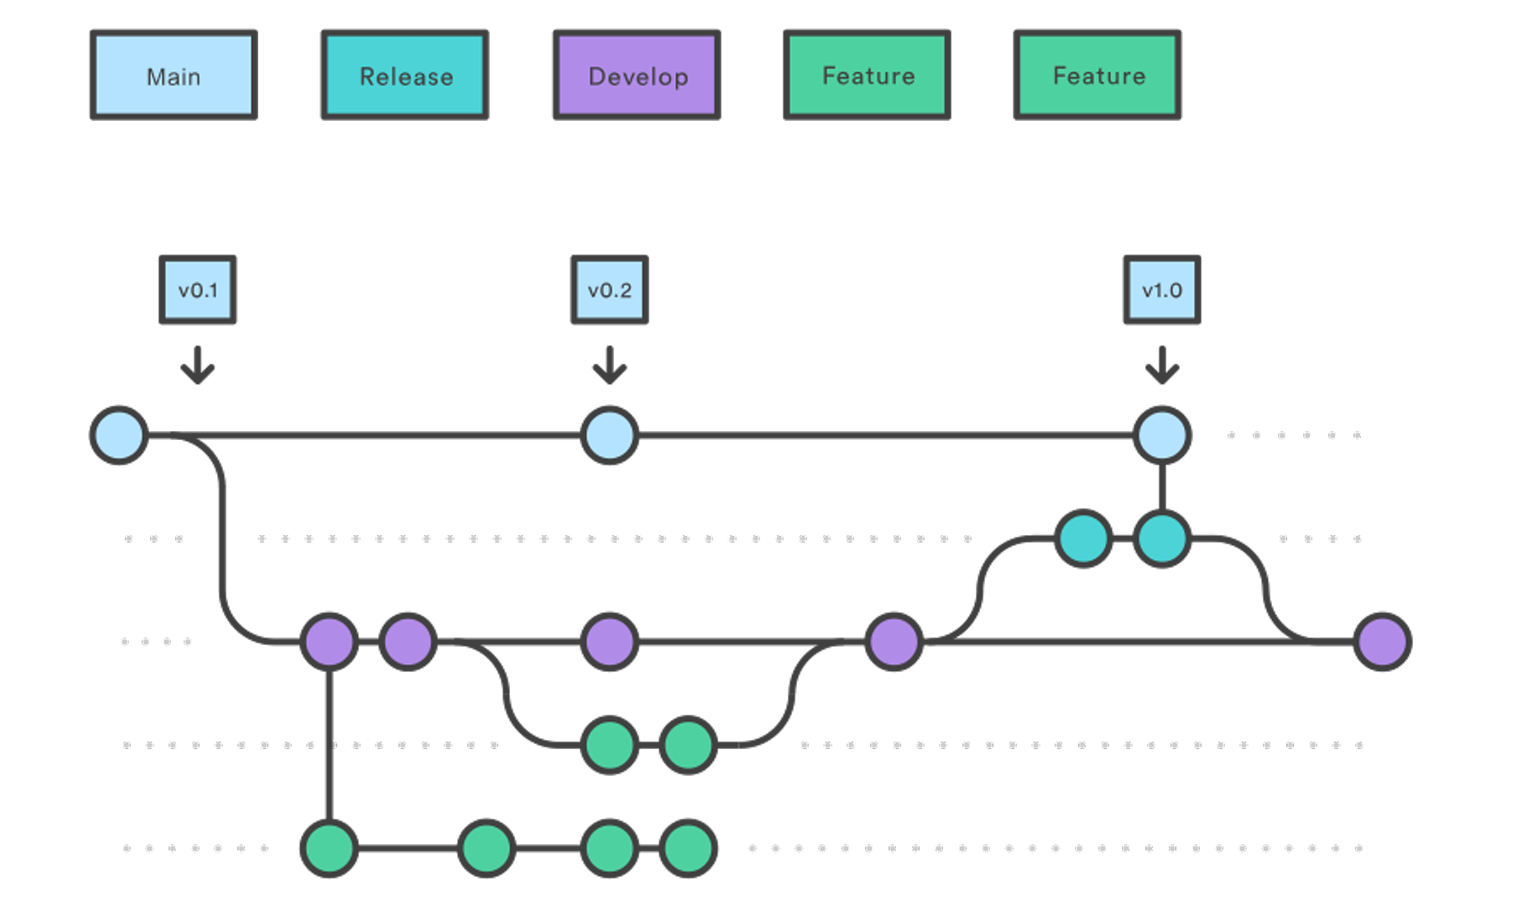
\includegraphics[width=0.9\textwidth]{images/gitWorkflow.png}
    \caption{Git Workflow}
    \label{fig:git-workflow}
\end{figure}

For each new feature or bug fix, we create a feature branch from develop. Once the work is completed and tested, it is merged back into develop through a pull request process. This ensures code review and quality control before any changes are integrated. When a release is ready, develop is merged into main, creating a new stable version of the application.

\section{Product backlog}

The backlog was created before the sprints to plan the milestones and determine the content of each sprint based on project needs \cite{ProductBacklogGuide2024, SchwarzScrum2019}. It includes the following fields:
\begin{itemize}
    \item \textbf{Code:} The unique identifier of the task.
    \item \textbf{Theme:} The subject of a user story.
    \item \textbf{User Story:} A short description of the functionality requested by the client.
    \item \textbf{Priority:} A value indicating the importance of the functionality \cite{MoscowMethodology2021, CleggCaseMethod2004}.
    \begin{itemize}
        \item \textbf{Must:} The feature is essential and must be implemented.
        \item \textbf{Should:} The feature should be implemented if possible.
        \item \textbf{Could:} The feature is optional and may be deprioritized.
        \item \textbf{Won't:} The feature is not a priority at this time.
    \end{itemize}
\end{itemize}

Table \ref{tab:product-backlog} shows the product backlog for our Korpor project:

\begin{longtable}{|c|l|p{8cm}|c|}
    \caption{Korpor Product Backlog\label{tab:product-backlog}} \\
        \hline
        \textbf{Code} & \textbf{Theme} & \textbf{User story} & \textbf{Priority} \\
        \hline
    \endfirsthead
    
    \hline
    \endhead
    
    \hline \multicolumn{4}{|r|}{{Continued on next page}} \\ \hline
    \endfoot
    
    \hline
    \endlastfoot
    
    % Authentication & User Management section
    \multicolumn{4}{|c|}{\cellcolor{primary!15}\textbf{\textcolor{primary}{Authentication \& User Management}}} \\
    \hline
    PB001 & Authentication & As a user, I want to create an account and authenticate securely & Must \\
    \hline
    PB002 & User Management & As a user, I want to manage my profile information & Must \\
    \hline
    PB003 & Authentication & As a user, I want to securely reset my password & Must \\
    \hline
    PB004 & Admin Management & As a Super Admin, I want to manage admin accounts for different real estate companies & Should \\
    
    
    % Super Admin Features section
    \multicolumn{4}{|c|}{\cellcolor{primary!15}\textbf{\textcolor{primary}{Super Admin Features}}} \\
    \hline
    PB005 & Security & As a Super Admin, I want to monitor security and compliance across the platform & Could \\
    \hline
    PB006 & Configuration & As a Super Admin, I want to configure platform-wide features and settings & Could \\
    \hline
    PB007 & Analytics & As a Super Admin, I want to generate and analyze global performance reports & Could \\
    \hline
    PB008 & Moderation & As a Super Admin, I want to moderate content across the platform & Won't \\
    \hline
    PB009 & AI Integration & As a Super Admin, I want to chat with an AI assistant that can securely access database information & Could \\
    \hline
    


    % Admin Features section
    \multicolumn{4}{|c|}{\cellcolor{primary!15}\textbf{\textcolor{primary}{Admin Features}}} \\
    \hline
    PB010 & Listing Management & As an Admin, I want to manage real estate listings in my company & Must \\
    \hline
    PB011 & Agent Management & As an Admin, I want to oversee real estate agents and their permissions & Should \\
    \hline
    PB012 & Transaction Management & As an Admin, I want to track transactions and calculate agent commissions & Should \\
    \hline
    PB013 & Customer Service & As an Admin, I want to address investor inquiries and issues & Could \\
    \hline
    PB014 & Analytics & As an Admin, I want to access a comprehensive agency dashboard & Could \\
    \hline
    PB015 & AI Integration & As an Admin, I want to input property details and receive AI-powered valuation & Should \\
    \hline
    
    % Real Estate Agent Features section
    \multicolumn{4}{|c|}{\cellcolor{primary!15}\textbf{\textcolor{primary}{Real Estate Agent Features}}} \\
    \hline
    PB016 & Listing Management & As an Agent, I want to create and manage property listings & Must \\
    \hline
    PB017 & Investment Management & As an Agent, I want to handle investment and purchase requests & Could \\
    \hline
    PB018 & Data Management & As an Agent, I want to contribute data for AI-driven estimates & Could \\
    \hline
    PB019 & Customer Relations & As an Agent, I want to maintain client relationships and communications & Could \\
    \hline
    PB020 & Finance & As an Agent, I want to view my commissions on sales and rentals & Should \\
    \hline
    
    % Investor Features section
    \multicolumn{4}{|c|}{\cellcolor{primary!15}\textbf{\textcolor{primary}{Investor Features}}} \\
    \hline
    PB021 & Property Discovery & As an Investor, I want to browse available property listings & Must \\
    \hline
    PB022 & Search Functionality & As an Investor, I want to filter properties based on my preferences & Could \\
    \hline
    PB023 & Investment Process & As an Investor, I want to invest in properties through a simple process & Could \\
    \hline
    PB024 & Portfolio Management & As an Investor, I want to track my investment portfolio in real-time & Must \\
    \hline
    PB025 & Payment Processing & As an Investor, I want to make secure payments through various methods & Should \\
    \hline
    PB026 & AI Recommendations & As an Investor, I want to receive personalized property recommendations & Must \\
    \hline
    PB027 & AI Assistance & As an Investor, I want to consult an AI assistant for real estate legal questions & Could \\
    \hline
    PB028 & Financial Prediction & As an Investor, I want to see predictions of potential earnings & Could \\
    \hline
    PB029 & Finance Management & As an Investor, I want to manage my earnings and withdrawals & Could \\
    \hline
    
    % AI & Machine Learning Features section
    \multicolumn{4}{|c|}{\cellcolor{primary!15}\textbf{\textcolor{primary}{AI \& Machine Learning Features}}} \\
    \hline
    PB030 & AI System & As the System, I want to analyze user interactions for personalized recommendations & Must \\
    \hline
    PB031 & AI Prediction & As the System, I want to predict property valuations and rental prices & Should \\
    \hline
    PB032 & AI Forecasting & As the System, I want to forecast potential investment returns & Should \\
    \hline
    PB033 & NLP Integration & As the System, I want to provide real estate legal information via NLP & Could \\
    \hline
    PB034 & Security & As the System, I want to secure AI database access for authorized queries & Could \\
    \hline
    
    % Blockchain & Smart Contract Features section
    \multicolumn{4}{|c|}{\cellcolor{primary!15}\textbf{\textcolor{primary}{Blockchain \& Smart Contract Features}}} \\
    \hline
    PB035 & Blockchain & As the System, I want to create and manage virtual contracts for transactions \cite{WangBlockchainRealEstate2023} & Must \\
    \hline
    PB036 & Blockchain & As an Investor, I want my property investments to be secured via blockchain \cite{McKinseyBlockchainRE2023} & Must \\
    \hline
    PB037 & Blockchain Management & As an Admin, I want to verify and validate blockchain transactions & Should \\
    \hline
    PB038 & Data Integrity & As the System, I want to store transaction records immutably on blockchain & Must \\
    \hline
    PB039 & System Monitoring & As a Super Admin, I want to monitor blockchain health and performance & Should \\
    \hline
    
    % System & Security Features section
    \multicolumn{4}{|c|}{\cellcolor{primary!15}\textbf{\textcolor{primary}{System \& Security Features}}} \\
    \hline
    PB040 & Authentication & As the System, I want to automate authentication and session management & Should \\
    \hline
    PB041 & Notifications & As the System, I want to generate real-time notifications for relevant users & Could \\
    \hline
    PB042 & Data Consistency & As the System, I want to maintain transaction consistency across the platform & Should \\
    \hline
    PB043 & Security & As the System, I want to ensure secure communication between AI and database & Should \\
    \hline
    
    % DevOps & Infrastructure section
    \multicolumn{4}{|c|}{\cellcolor{primary!15}\textbf{\textcolor{primary}{DevOps \& Infrastructure}}} \\
    \hline
    PB044 & CI/CD & As a Developer, I want CI/CD pipelines to build project images on GitHub \cite{ForsgreniDevOpsMetrics2023} & Must \\
    \hline
    PB045 & Deployment & As a Developer, I want to automate image deployment to GCP registry & Must \\
    \hline
    PB046 & Deployment & As a Developer, I want to auto-deploy backend services and database & Must \\
    \hline
    PB047 & Containerization & As a Developer, I want to containerize application components with Docker & Must \\
    \hline
    PB048 & Web Deployment & As a Developer, I want to automatically deploy the web app frontend & Should \\
    \hline
    PB049 & Mobile Deployment & As a Developer, I want to automate mobile app deployments to Play Store & Should \\
    \hline
    PB050 & Versioning & As a Developer, I want to implement versioning for mobile app releases & Should \\
    \hline
    PB051 & Monitoring & As an Admin, I want to monitor system health and performance & Could \\
    \hline
    PB052 & Configuration & As a Super Admin, I want to manage environment configurations & Could \\
        \hline
    
    % Mobile App Specific Features section
    \multicolumn{4}{|c|}{\cellcolor{primary!15}\textbf{\textcolor{primary}{Mobile App Specific Features}}} \\
    \hline
    PB053 & Mobile UI/UX & As an Investor, I want a responsive, intuitive mobile interface \cite{NielsenResponsiveDesign2019} & Should \\
    \hline
    PB054 & Notifications & As an Investor, I want to receive push notifications about my investments & Should \\
    \hline
    PB055 & Offline Access & As an Investor, I want offline access to my basic portfolio information & Should \\
\end{longtable}

\section{Sprint planning}

In order to complete the project within the deadlines set by the internship agreement, planning is an important step in the process \cite{SutherlandScrum2020, RubinEssentialScrum2012}. It was therefore necessary to define the essential steps and estimate the time to be devoted to the completion of the various tasks. To do this, we made a GANTT chart.

In our project management, we opted for the proportional distribution method in order to estimate the costs \cite{CohnAgileEstimating2005, GreningPlanningPoker2002}.
Figure \ref{fig:gantt-chart} shows the Gantt chart that describes the progress of our project:

\vspace{1cm}
\newpage

\begin{figure}[htbp]
    \centering
    % Replace with actual image file once available
    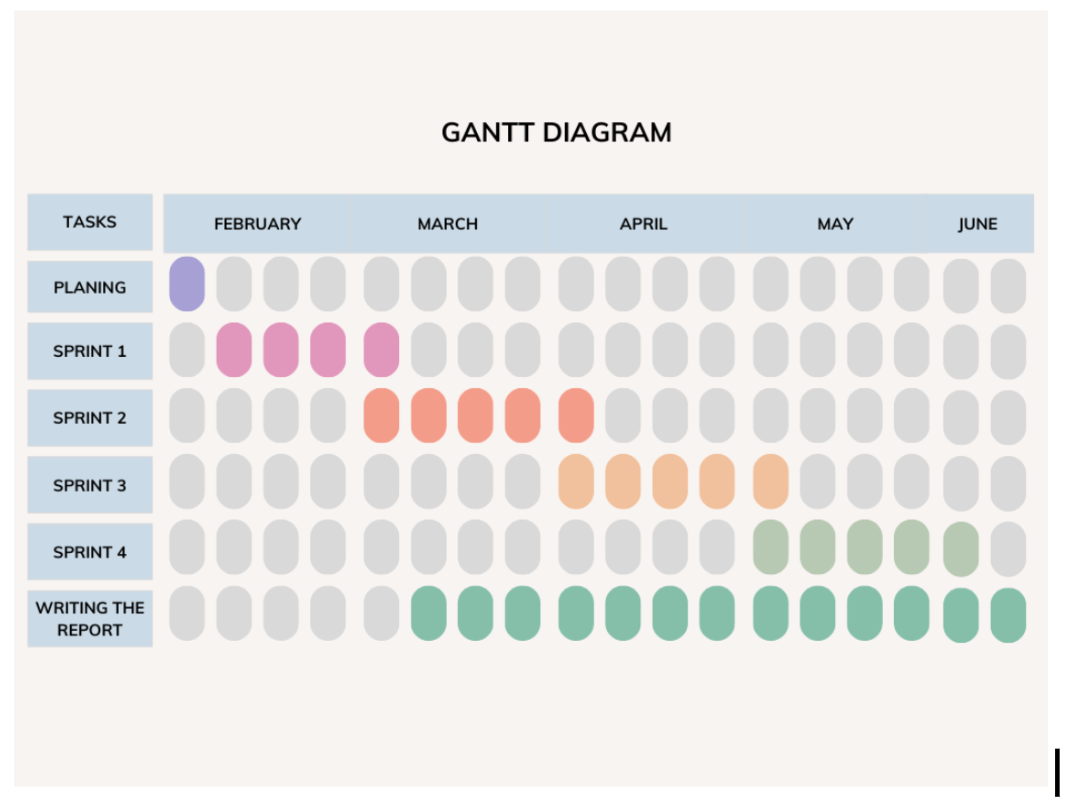
\includegraphics[width=0.7\textwidth]{images/gantt-chart.png}
    \caption{GANTT chart with sprint planning}
    \label{fig:gantt-chart}
\end{figure}

% \vspace{2cm}

\section*{Conclusion}

Our Sprint 0 marked the exciting start of our KORPOR project \cite{ScaledAgileFramework2024, SutherlandScrum2020}. We defined global and specific objectives, developed a solid architecture, and configured an optimal working environment. With a clear vision of the initial product backlog and preliminary planning for upcoming sprints, we are ready to achieve our vision and achieve our goals successfully \cite{SchwarzScrum2019, RubinEssentialScrum2012}.


\cleardoublepage

% Insert page break in TOC before Chapter 3
% \addtocontents{toc}{\protect\newpage}

% Chapter 3: Design and Implementation
\chapter{AUTHENTICATION \& USER MANAGEMENT}
\vspace{-0.5cm}
\section*{Introduction}
\addcontentsline{toc}{section}{Introduction}
This chapter presents the authentication and user management system, which forms the security foundation of the Korpor platform. The implementation covers user registration, role-based access control, and comprehensive authentication workflows for both web and mobile interfaces.

 
\section{Sprint 1: Authentication and User Management}

\subsection*{Introduction}
The first sprint focuses on establishing the core authentication system and user management functionality. This foundation is critical for all subsequent features as it defines user roles and access controls.

\subsection{Analysis}
The Authentication and User Management system underpins Korpor's security and user access. It covers registration with roles, secure login, password recovery, and session management. Figure~\ref{fig:auth-usermgmt-usecase} shows the main use cases.
\newpage
\begin{figure}[htbp]
    \centering
    % Replace with actual image file path
    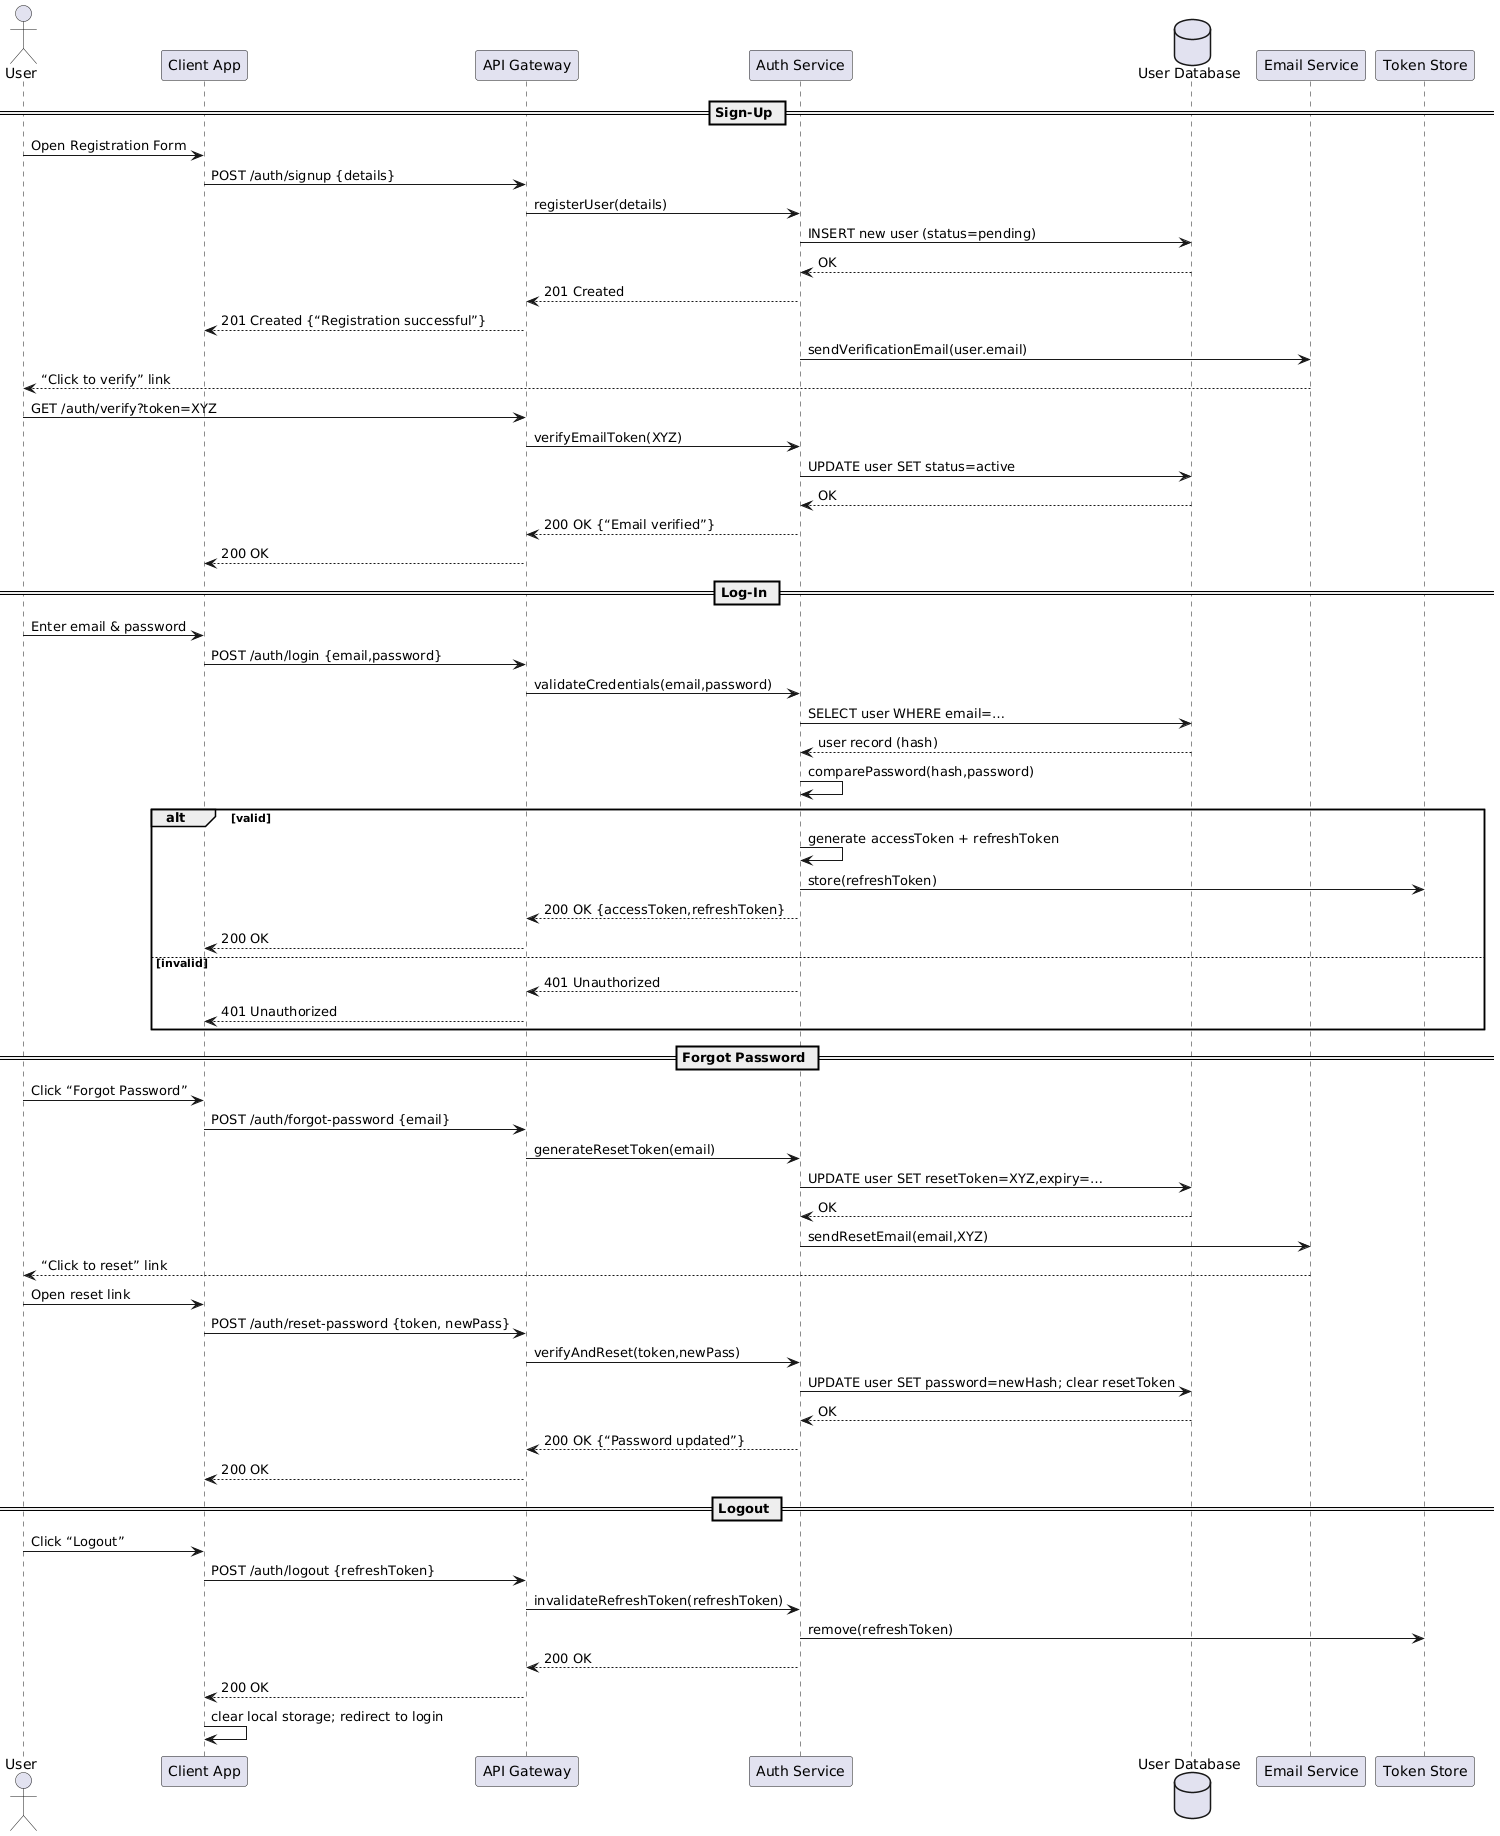
\includegraphics[width=0.9\textwidth]{images/auth-usermgmt-usecase.png} 
    \caption{Global Use Case Diagram for Authentication and User Management}
    \label{fig:auth-usermgmt-usecase}
\end{figure}


\subsubsection{Sign-up Process}
% The sign-up process is illustrated in Figure \ref{fig:signup-diagram} below. The diagram shows the authentication flow for new users registering in the system.

% \begin{figure}[ht!]
%     \centering
%     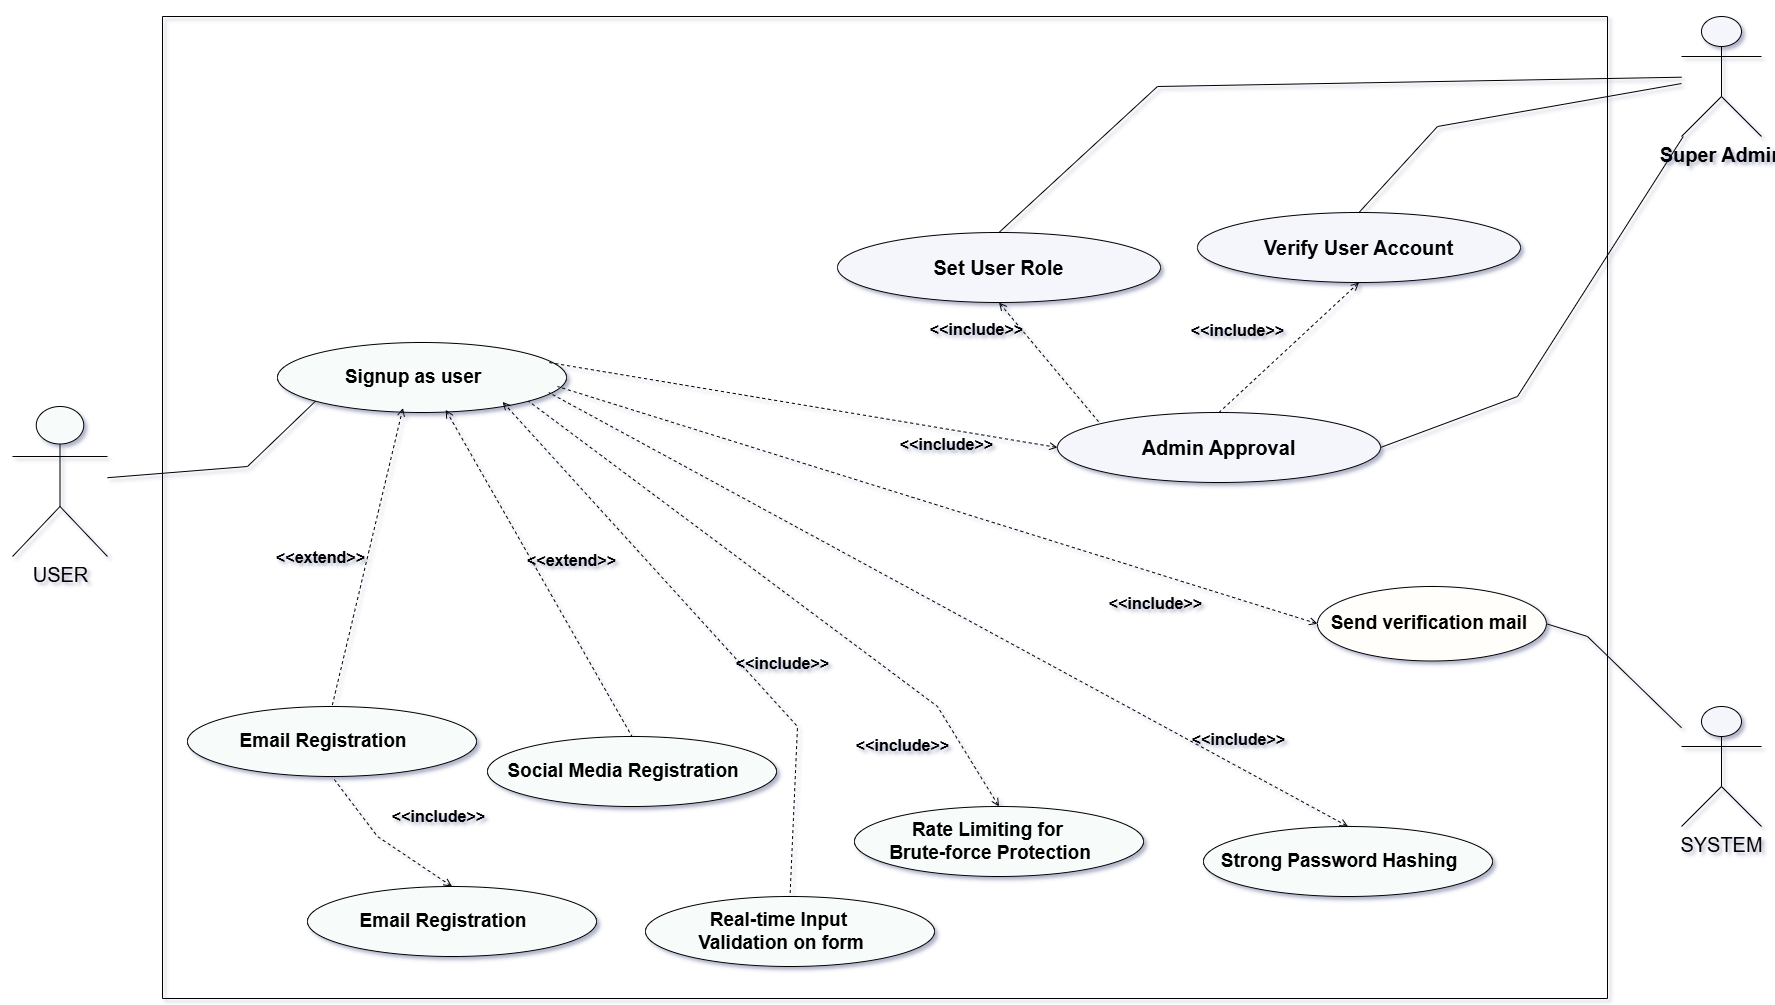
\includegraphics[width=1.03\textwidth]{images/diagram_de_case_d_utilisation_signup.png}
%     \caption{Authentication Sign-up Use Case Diagram}
%     \label{fig:signup-diagram}
% \end{figure}

\begin{table}[htbp]
    \centering
    \begin{tabular}{|p{4cm}|p{9cm}|}
        \hline
        \textbf{Step} & \textbf{Description} \\
        \hline
        Start Sign-Up & User navigates to the sign-up page and presses the sign-up button. \\
        \hline
        Fill Form & System presents a form for the user to complete. \\
        \hline
        Validate Information & Upon submission, the system validates the entered information. \\
        \hline
        Invalid Information & If invalid, user is prompted to correct the form. \\
        \hline
        Valid Information & If valid, system saves user details and sends a verification email. \\
        \hline
        Email Verification & User checks their email and verifies their account. \\
        \hline
        Verification Success & System redirects user to an email verification code page or confirmation step. \\
        \hline
        Super Admin Review & Super Admin performs a two-step verification: \\
        \hline
        Verification Failure & If email verification fails, an error message is displayed. \\
        \hline
    \end{tabular}
    \caption{Sign-Up Activity Flow}
    \label{tab:signup-activity-flow}
\end{table}




% \subsubsection{Manage Users Process}
% The user management process enables administrators to create, view, update, and delete user accounts. The table below details the use case, as shown in Table \ref{tab:manage_users_process}.


% \begin{table}[htbp]
%     \centering
%     \begin{tabular}{|l|p{0.7\textwidth}|}
%         \hline
%         \textbf{Section} & \textbf{Details} \\
%         \hline
%         Use Case & Assign Role \\
%         \hline
%         Actor & Super Admin \\
%         \hline
%         Precondition & Actor is logged into the system with appropriate administrative privileges. \\
%         \hline
%         Main Scenario & 
%         Super Admin assigns a role to a user. \\
%         \hline
%         Postcondition & User account is created, updated, or deleted as per the action taken. The list of users reflects the changes. \\
%         \hline
%         Exception & 
%         - Invalid input data: System displays validation errors.
%         - Permission denied: System prevents unauthorized actions.
%         - User not found (for update/delete): System displays an error message.
%         - System error: System displays a general error message. \\
%         \hline
%     \end{tabular}
%     \caption{Manage Users Process Details}
%     \label{tab:manage_users_process}
% \end{table}




\subsection{Modeling}

Figure \ref{fig:auth-class-diagram} depicts the class diagram for the authentication system. It showcases the key components and their relationships involved in user authentication and authorization.
\newpage
\begin{figure}[htbp]
    \centering
    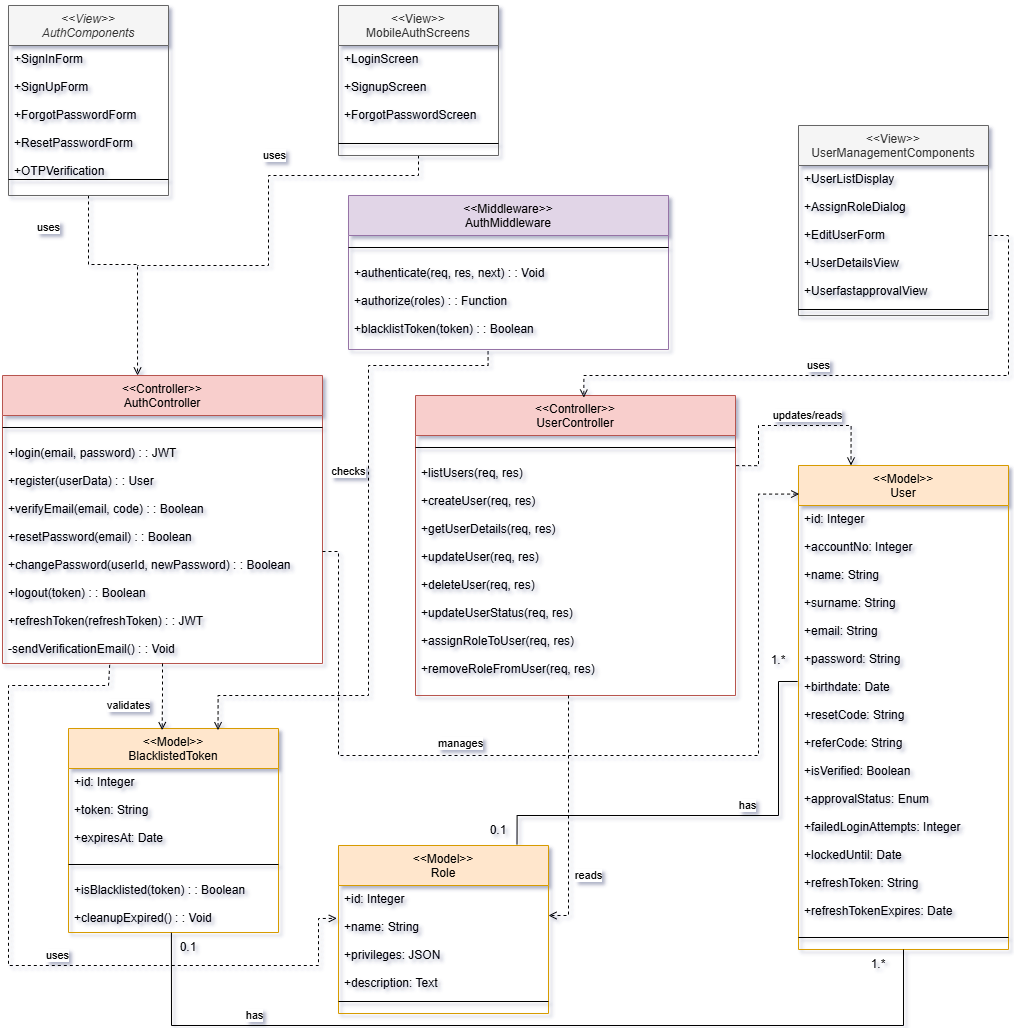
\includegraphics[width=1\textwidth]{images/auth_classdiag.PNG}
    \caption{Authentication AND User Management System Class Diagram}
    \label{fig:auth-class-diagram}
\end{figure}


\begin{itemize}
    \item \textbf{AuthComponents}: Represents the UI elements for authentication, such as SignInForm, SignUpForm, ForgotPasswordForm, ResetPasswordForm, and OTPVerification. These components are used by \textbf{MobileAuthScreens}.
    \item \textbf{MobileAuthScreens}: Includes screens like LoginScreen, SignupScreen, and ForgotPasswordScreen that utilize \textbf{AuthComponents} and interact with the \textbf{AuthService}.
    \item \textbf{AuthService}: Acts as an intermediary between the frontend components/screens and the backend. It handles functions like signIn, signUp, verifyEmail, forgotPassword, resetPassword, logout, refreshToken, and error handling. It consumes \textbf{AuthRoutes}.
    \item \textbf{AuthRoutes}: Defines the API endpoints for authentication, such as /login, /register, /verify-email, /forgot-password, /reset-password, /logout, and /refresh-token. These routes map to methods in the \textbf{AuthController}.
    \item \textbf{AuthController}: Contains the core logic for authentication processes, including login, register, verifyEmail, resetPassword, changePassword, logout, refreshToken, and sendVerificationEmail. It interacts with the \textbf{User}, \textbf{Role}, and \textbf{BlacklistedToken} models and utilizes \textbf{AuthMiddleware}.
    \item \textbf{AuthMiddleware}: Provides middleware functions for authentication (authenticate) and authorization (authorize roles). It also manages blacklisted tokens (blacklistToken) and interacts with the \textbf{User} model.
    \item \textbf{User}: Represents the user entity with attributes like id, accountNo, name, surname, email, password, birthdate, resetCode, isVerified, approvalStatus, failedLoginAttempts, lockedUntil, refreshToken, and refreshTokenExpires. A User has one or more \textbf{Role}s.
    \item \textbf{Role}: Defines user roles with attributes like id, name, privileges (JSON), and description. Each User is associated with a Role (0..1 relationship shown, typically a User has at least one Role, but the diagram indicates a User can have zero or one Role, which might need clarification or represent a specific system design choice, e.g., a default role or a user awaiting role assignment).
    \item \textbf{BlacklistedToken}: Stores tokens that have been invalidated (e.g., after logout or password change) with attributes like id, token, and expiresAt. It includes methods like isBlacklisted and cleanupExpired. The \textbf{AuthController} uses this to validate tokens, and \textbf{AuthMiddleware} checks against it.
\end{itemize}

\subsection{Implementation}
The implementation of the authentication and user management system resulted in the following key user interfaces:

\subsubsection{Sign-in Interface}
The sign-in interface provides a secure and user-friendly means for users to authenticate. Figure \ref{fig:signin-interface} shows the implementation of this interface.
\newpage
\begin{figure}[htbp]
    \centering
    % Add correct path when available
    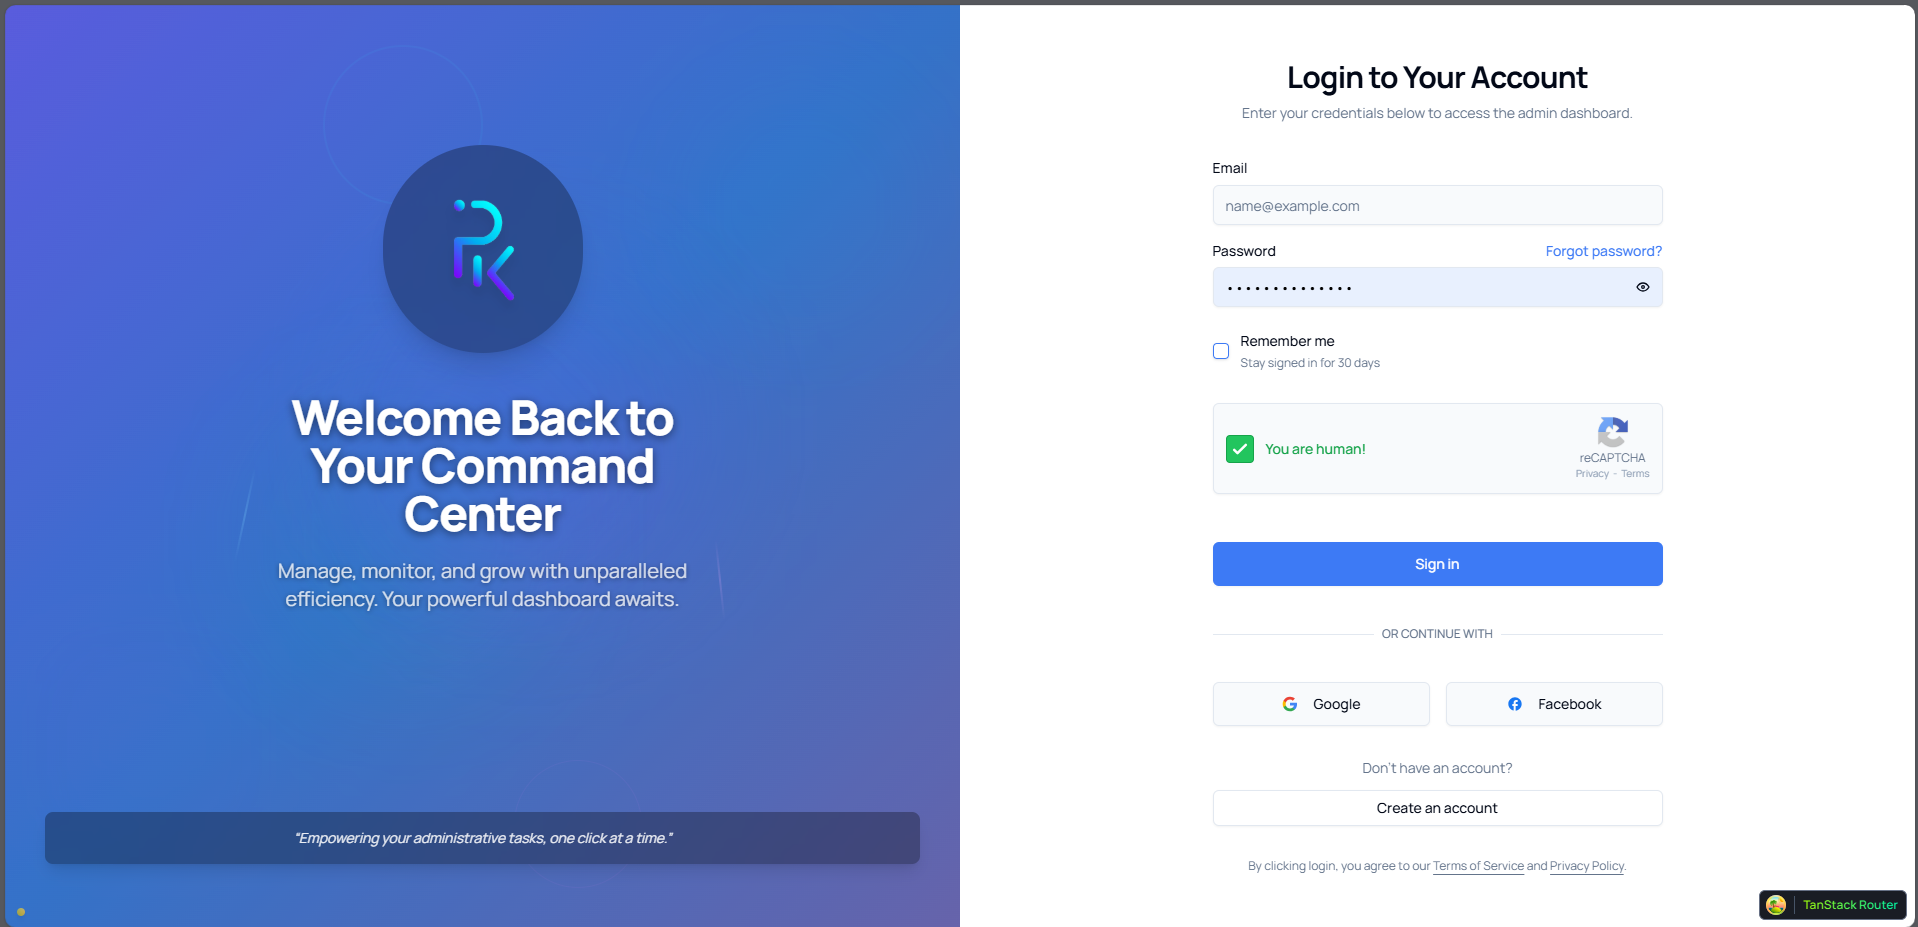
\includegraphics[width=1\textwidth]{images/signin-interface.png}
    \caption{Sign-in Interface Implementation}
    \label{fig:signin-interface}
\end{figure}

\subsubsection{Sign-up Interface}
The sign-up interface allows new users to register for an account. It collects necessary information and begins the verification process. Figure \ref{fig:signup-interface} displays this implementation.

\begin{figure}[htbp]
    \centering
    % Add correct path when available
    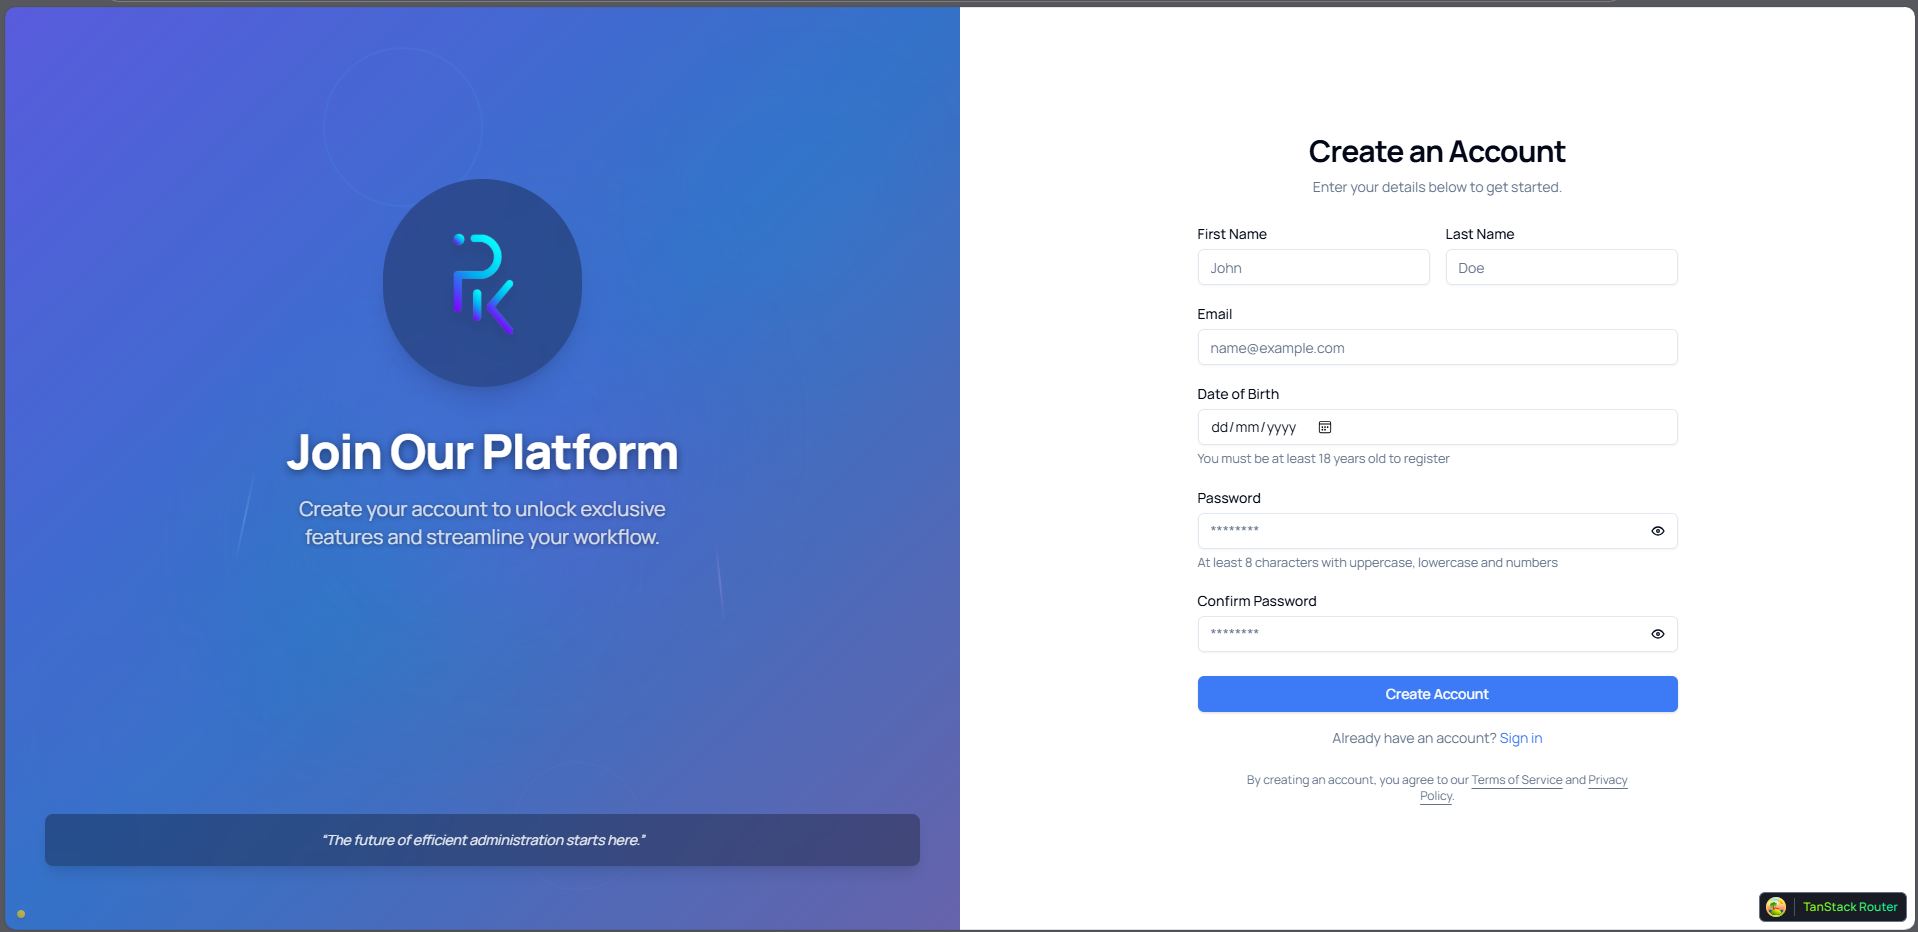
\includegraphics[width=1\textwidth]{images/signup-interface.png}
    \caption{Sign-up Interface Implementation}
    \label{fig:signup-interface}
\end{figure}

\subsubsection{User Management in Super Admin Dashboard}
The Super Admin dashboard provides comprehensive user management capabilities, including the ability to view, create, edit, and deactivate user accounts. Figure \ref{fig:user-management} shows this powerful interface.
\newpage
\begin{figure}[htbp]
    \centering
    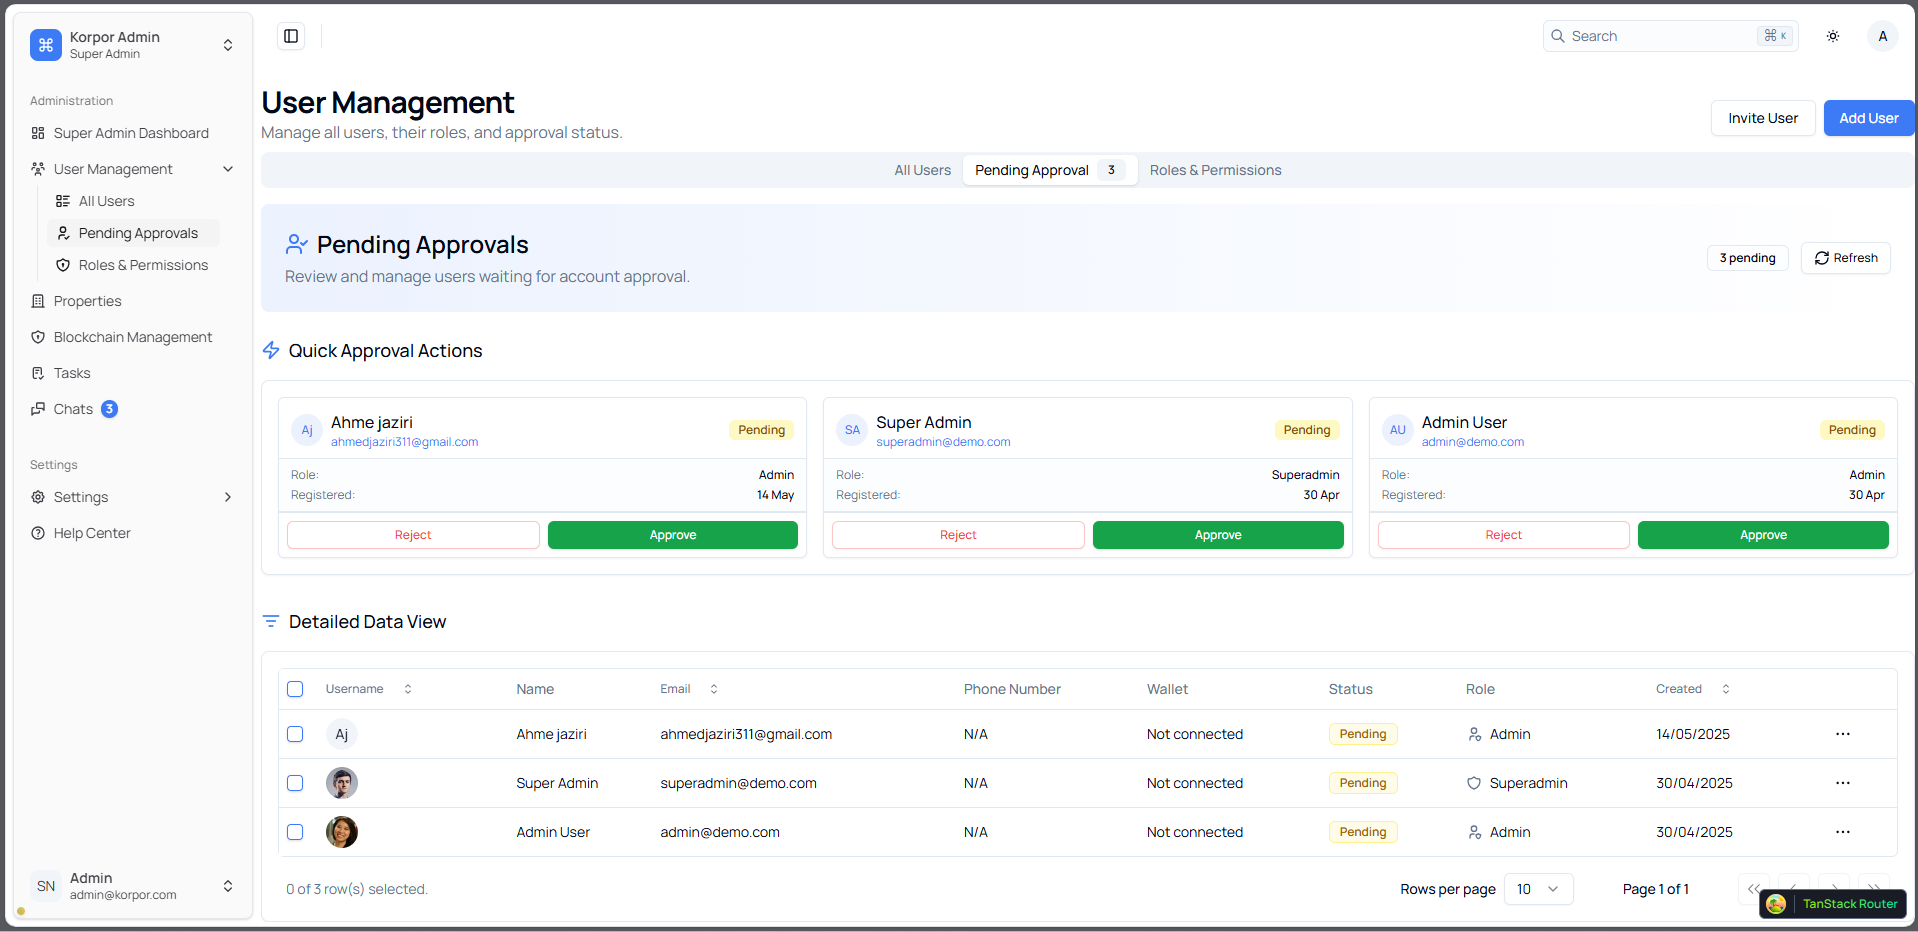
\includegraphics[width=1\textwidth]{images/user-management-dashboard.png}
    \caption{User Management Interface in Super Admin Dashboard}
    \label{fig:user-management}
\end{figure}

The mobile application provides a streamlined authentication experience for investors. The system includes comprehensive error handling to guide users through common authentication issues, as shown in Figure \ref{fig:mobile-auth-errors}. The complete authentication flow includes login, signup, OTP verification, and password recovery interfaces designed for clarity and ease of use on mobile devices, as shown in Figure \ref{fig:mobile-auth-interfaces}.
\begin{figure}[htbp]
    \centering
    \begin{subfigure}[b]{0.45\textwidth}
        \centering
        
\includegraphics[width=\textwidth]{images/mobile-auth-screen_invalidemailorpass.png}
        \caption{Invalid Email or Password Error}
        \label{fig:mobile-invalid-credentials}
    \end{subfigure}
    \hfill
    \begin{subfigure}[b]{0.45\textwidth}
        \centering
        
\includegraphics[width=\textwidth]{images/mobile-auth-screen_emptyfieldsmessage.png}
        \caption{Empty Fields Validation Error}
        \label{fig:mobile-empty-fields}
    \end{subfigure}
    \caption{Authentication Validation Messages}
    \label{fig:mobile-auth-errors}
\end{figure}
% \subsubsection{Complete invastor Authentication Flow}
\newpage 

\begin{figure}[htbp]
    \centering
    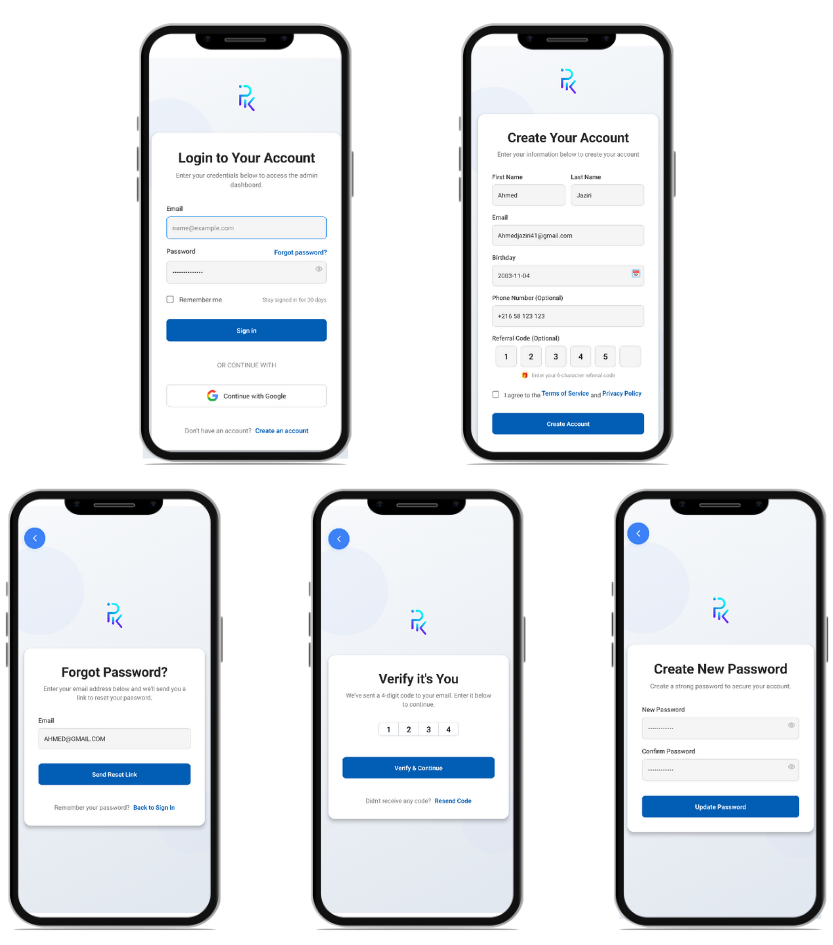
\includegraphics[width=1\textwidth]{images/mobile auth.png}
    \caption{Complete Mobile Application Authentication Flow}
    \label{fig:mobile-auth-interfaces}
\end{figure}

\newpage

\subsection{Test}
To ensure the reliability and functionality of the authentication and user management system, we implemented comprehensive testing using Playwright, an end-to-end testing framework.

\subsubsection{Playwright Test Results}
The authentication system underwent rigorous testing through automated test scripts that verified all key functionality, including sign-up, sign-in, password reset, and user management operations. Figure \ref{fig:playwright-tests} demonstrates the successful execution of these tests.
\begin{figure}[htbp]
    \centering
    % Add correct path when available
    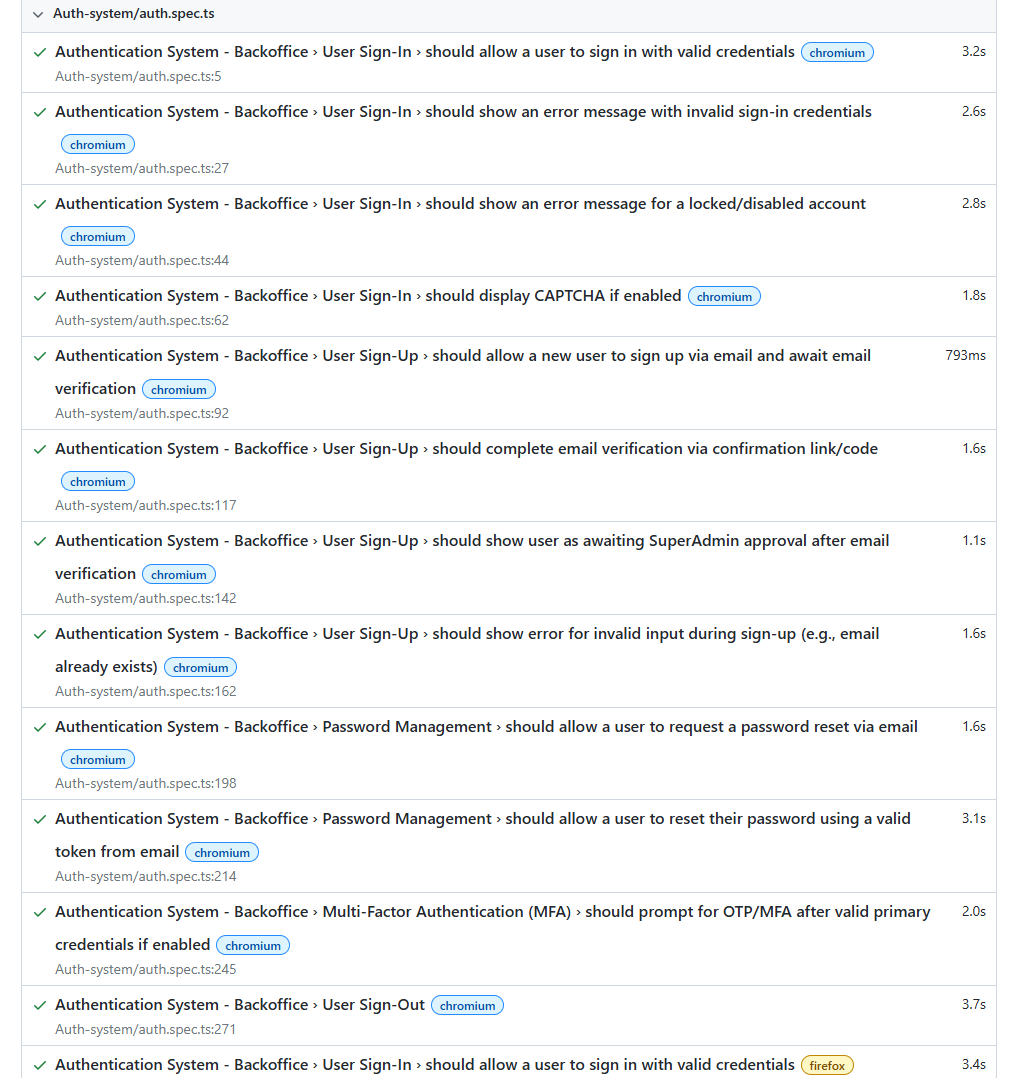
\includegraphics[width=0.65\textwidth]{images/playwright-test-results.png}
    \caption{Playwright Test Results for Authentication System}
    \label{fig:playwright-tests}
\end{figure}


All tests passed successfully, confirming the robustness of the implemented authentication system.
\newpage
\subsection{Retrospective}

The authentication and user management sprint provided valuable insights into system development and team collaboration. Table \ref{tab:auth-retrospective} summarizes the key achievements, challenges, and lessons learned during this sprint.
\begin{table}[htbp]
    \centering
    \begin{tabular}{|p{3cm}|p{10cm}|}
        \hline
        \textbf{Category} & \textbf{Details} \\
        \hline
        \textbf{What Went Well} & 
        \begin{itemize}
            \item Successfully implemented secure authentication flow
            \item Role-based access control working as expected
            \item Mobile interface provides excellent user experience
            \item All planned test scenarios passed
            \item Strong team collaboration throughout the sprint
        \end{itemize} \\
        \hline
        \textbf{Challenges} & 
        \begin{itemize}
            \item Initial complexity in setting up JWT token management
            \item Integration testing required more time than estimated
            \item Email verification system configuration challenges
            \item Balancing security requirements with user experience
        \end{itemize} \\
        \hline
    \end{tabular}
    \caption{Authentication Sprint Retrospective Summary}
    \label{tab:auth-retrospective}
\end{table}

\section*{Conclusion}

The Foundation sprint successfully established the secure authentication and user management infrastructure for the Korpor platform.

% Additional sections for subsequent sprints will be added later 
\cleardoublepage

% Main Matter (Page numbering already set to arabic)
% \chapter{Project Context}
% \input{chapters/project_context.tex}

% \chapter{Introduction} % Example for later
% \input{chapters/introduction.tex}

% Chapter 4:
% Chapter 4: Artificial Intelligence Features
\chapter{Artificial Intelligence Features}

\chapterquote{Artificial intelligence is the new electricity.}{Andrew Ng}

\section*{Introduction}
\addcontentsline{toc}{section}{Introduction}

This chapter explores the integration of artificial intelligence capabilities within our real estate platform. We have developed four distinct AI models, each addressing specific requirements within the ecosystem. These models collectively enhance user experience, improve decision-making processes, and provide valuable insights to various stakeholders in the real estate market.

The AI features presented in this chapter represent a significant competitive advantage for our platform, enabling more accurate property valuations, personalized recommendations, intelligent assistance, and efficient administrative operations. Each model has been carefully designed to solve real-world challenges faced by users interacting with real estate data and transactions.

\section{Sprint 2: Data Collection and Scraping}
\subsection*{Overview}
This section details the data collection processes implemented to gather the real estate market data required for our AI models. 

\subsection{Real Estate Data Scraping}
\subsubsection{Data Sources}
We identified several real estate websites with
significant listings for the Tunisian market: Properstar, Remax, Home in Tunisia, and
Mubawab. These platforms offered a reasonable volume of property listings with the
attributes needed for our models. For each website, I developed a dedicated Python
script that navigated through the listings, extracted the relevant property details, and
stored the information in CSV files. This approach gave us a foundation of raw data that
could later be processed and used for training our prediction models.
\newpage
\begin{figure}[htbp]
    \centering
    \begin{minipage}{0.47\textwidth}
        \centering
        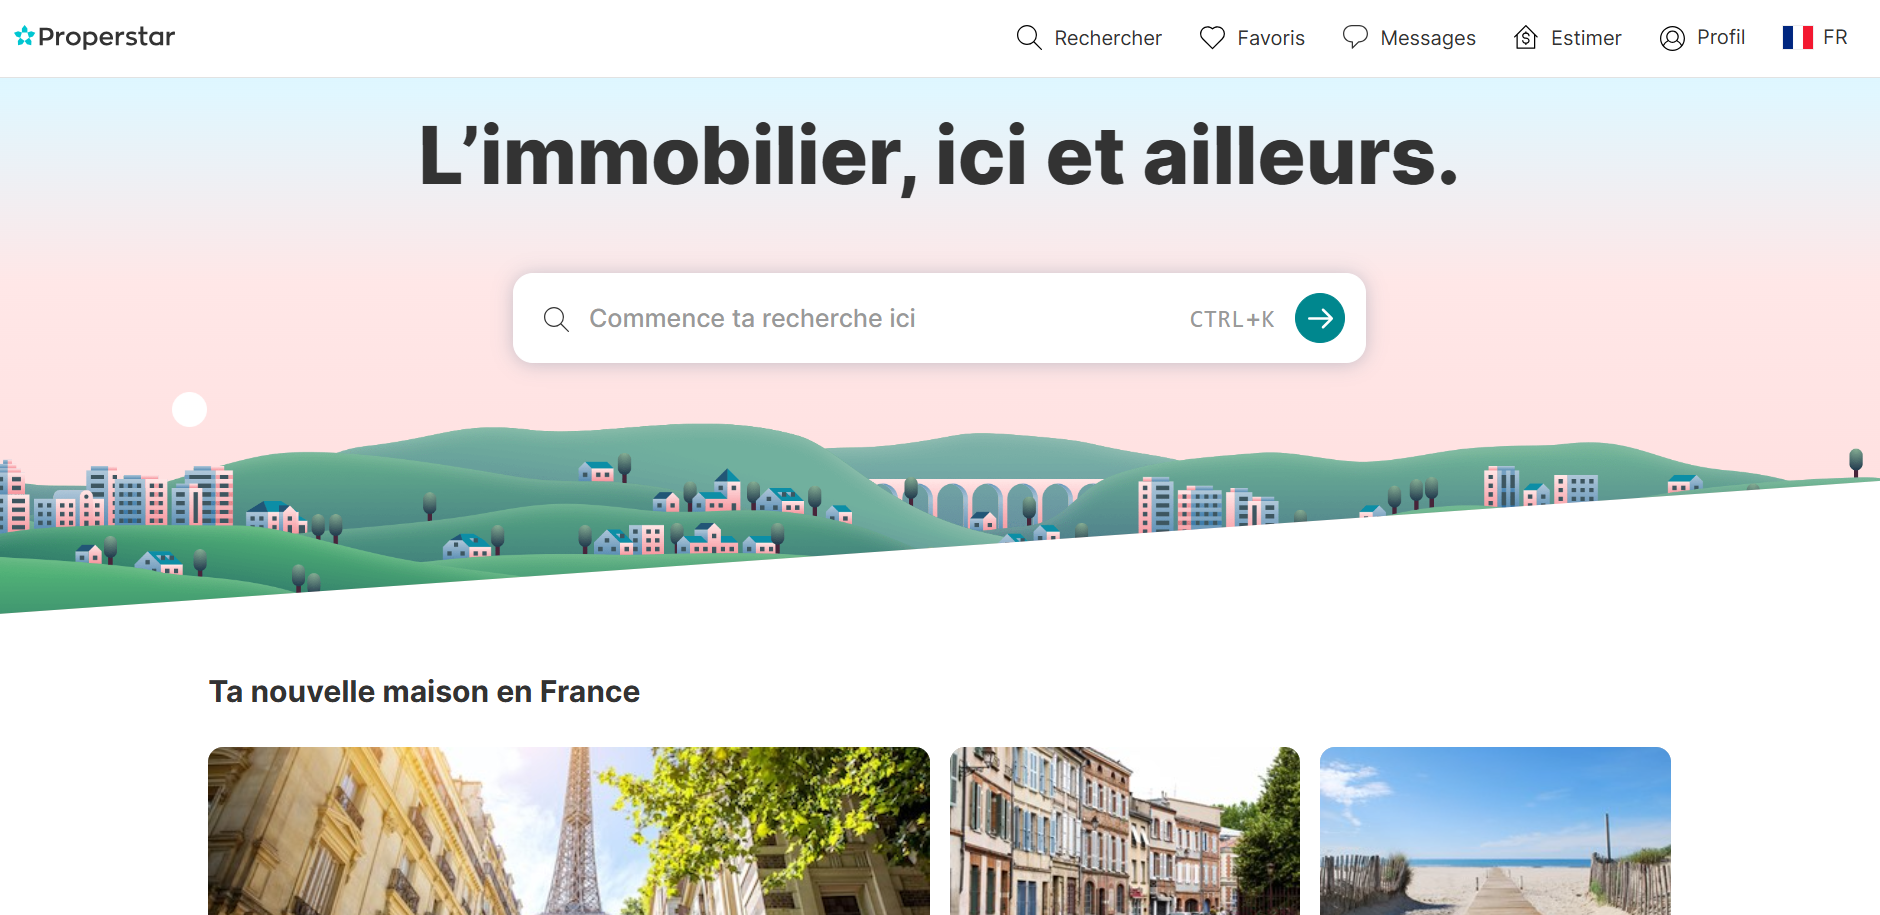
\includegraphics[width=\linewidth]{images/properstar.png}
        \caption{properstar website}
        \label{fig:properstar-website}
    \end{minipage}
    \hfill
    \begin{minipage}{0.47\textwidth}
        \centering
        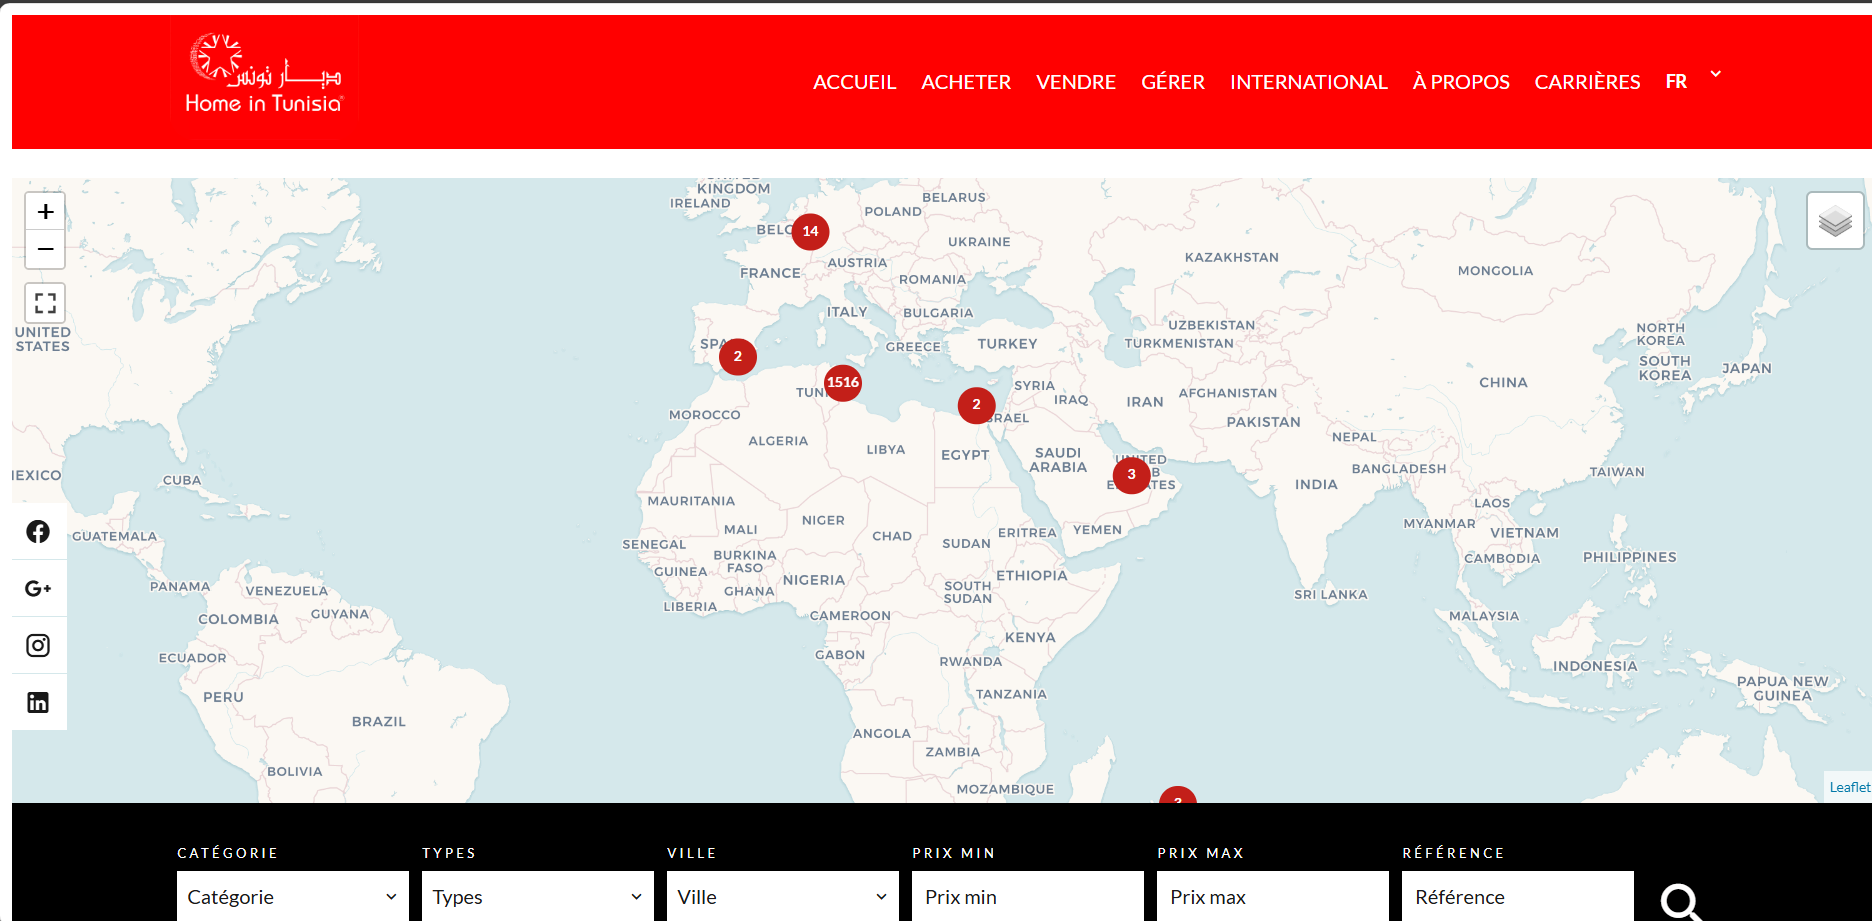
\includegraphics[width=\linewidth]{images/home_in_tunisia.png}
        \caption{homeintunisia website}
        \label{fig:homeintunisia-website}
    \end{minipage}
    
    \vspace{0.75cm}
    
    \begin{minipage}{0.47\textwidth}
        \centering
        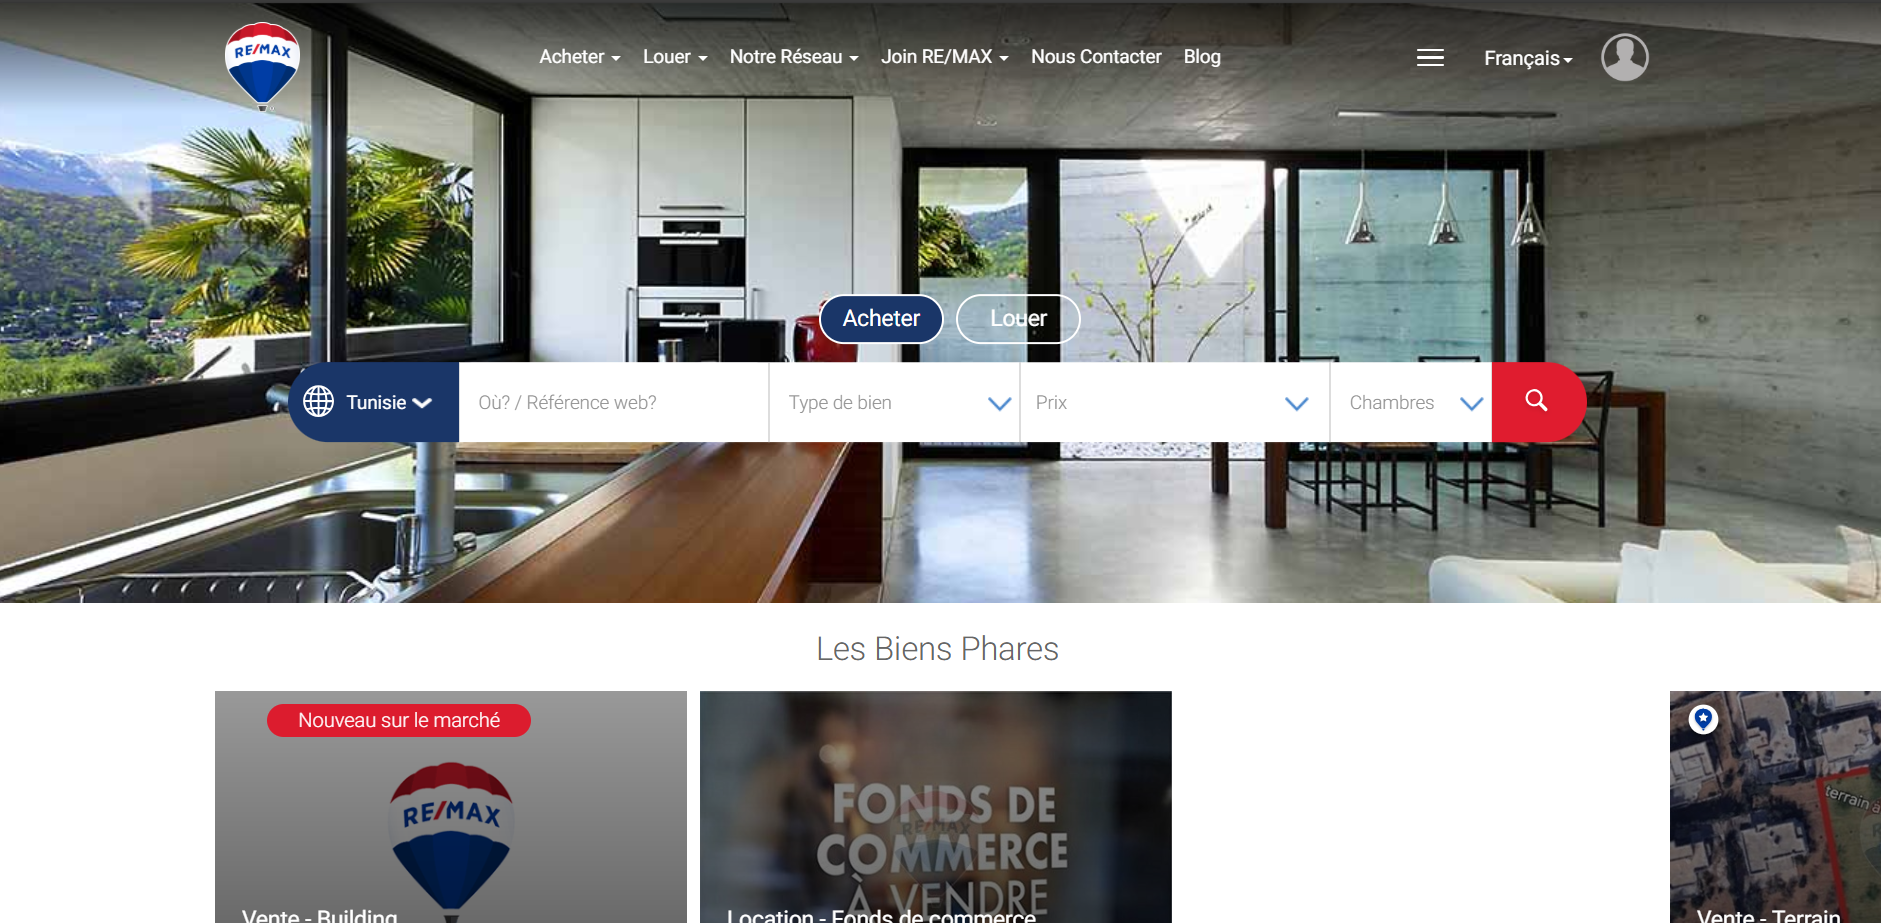
\includegraphics[width=\linewidth]{images/remax.png}
        \caption{remax website}
        \label{fig:remax-website}
    \end{minipage}
    \hfill
    \begin{minipage}{0.47\textwidth}
        \centering
        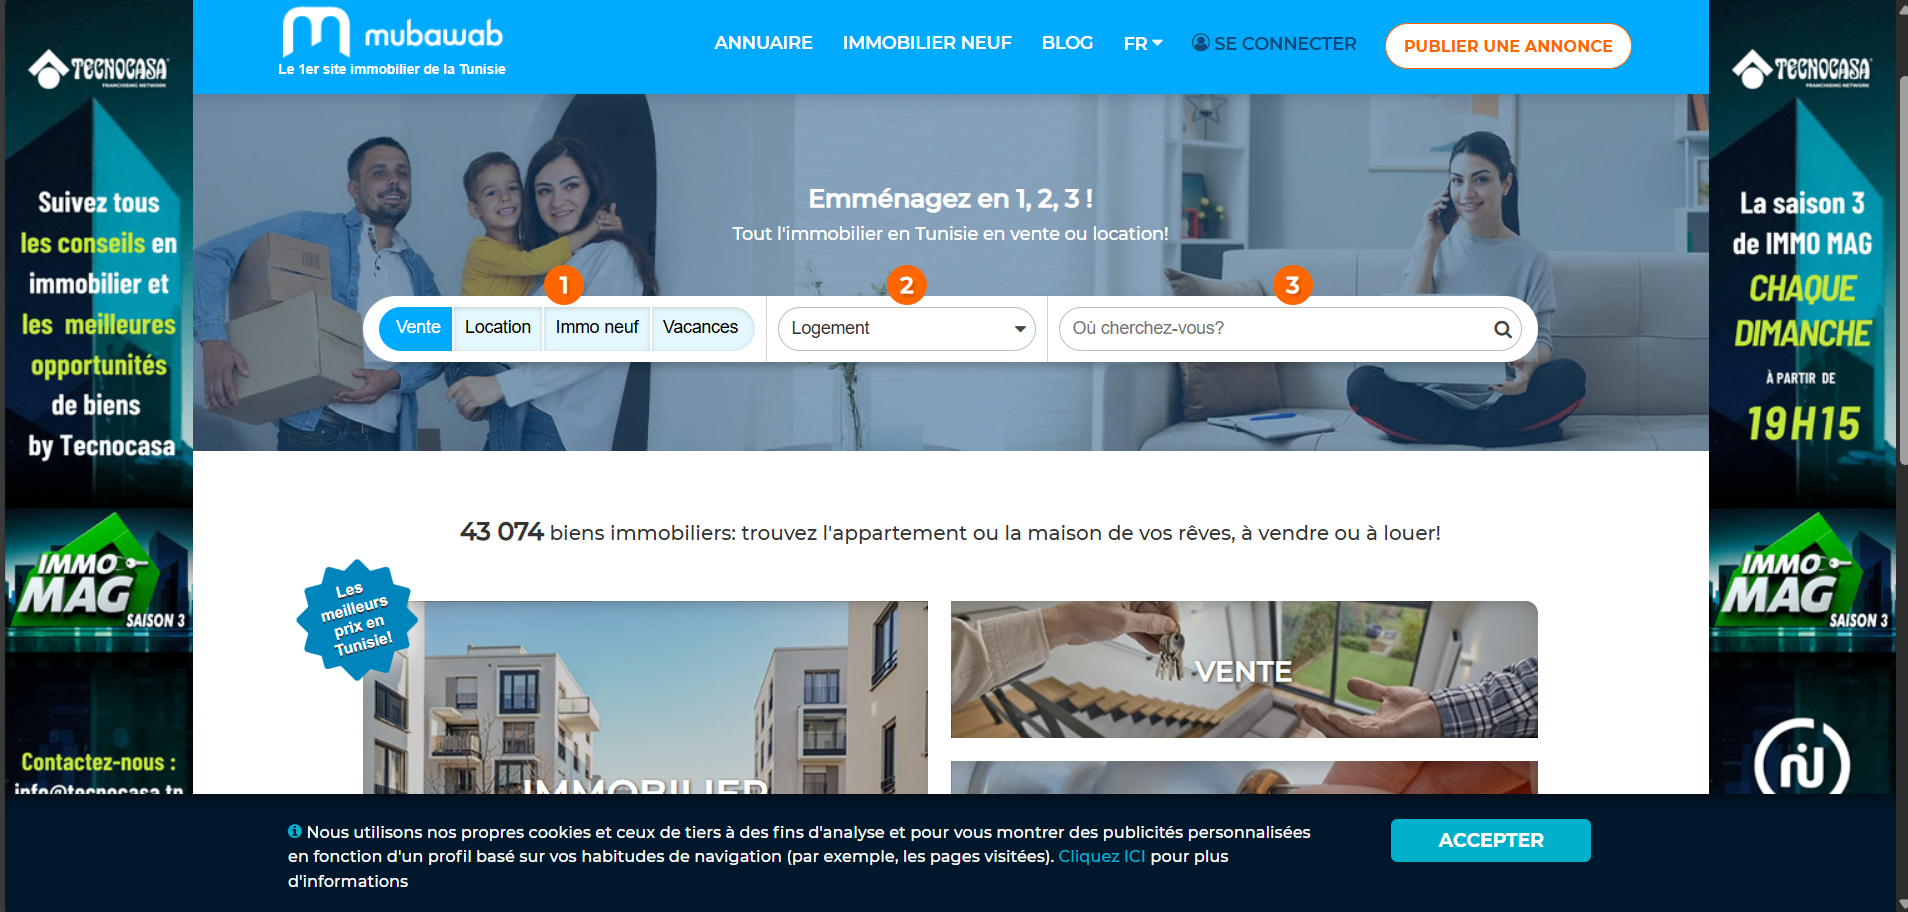
\includegraphics[width=\linewidth]{images/mub.png}
        \caption{mubawab website}
        \label{fig:mubawab-website}
    \end{minipage}
\end{figure}

Our scraping system uses a distributed architecture with the following components:
\begin{itemize}
    \item Scheduled jobs for regular data updates, Data validation and cleaning pipelines
\end{itemize}

\begin{figure}[htbp]
    \centering
    % Placeholder for a diagram of the scraping workchart
    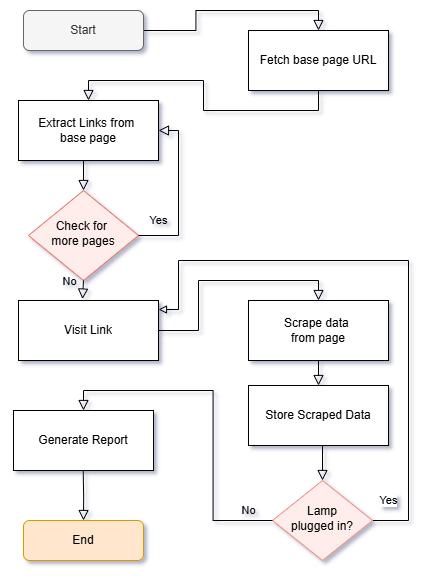
\includegraphics[width=0.35\textwidth]{images/workchartscraper.png}
    \caption{Data Scraping workchart}
    \label{fig:scraping-workchart}
\end{figure}

\section{Sprint 3: Property Valuation Prediction Model}
\subsection*{Overview}
The Property Valuation Prediction Model is designed to estimate both the market value and potential rental income for real estate properties. This provides investors with crucial information to make informed investment decisions.

\subsection{Requirements Analysis}
\subsubsection{Use Case Diagram}
The property valuation model serves multiple actors within the Korpor ecosystem. Figure \ref{fig:valuation-use-case} illustrates the primary use cases for the AI-powered property valuation system.

\begin{figure}[htbp]
    \centering
    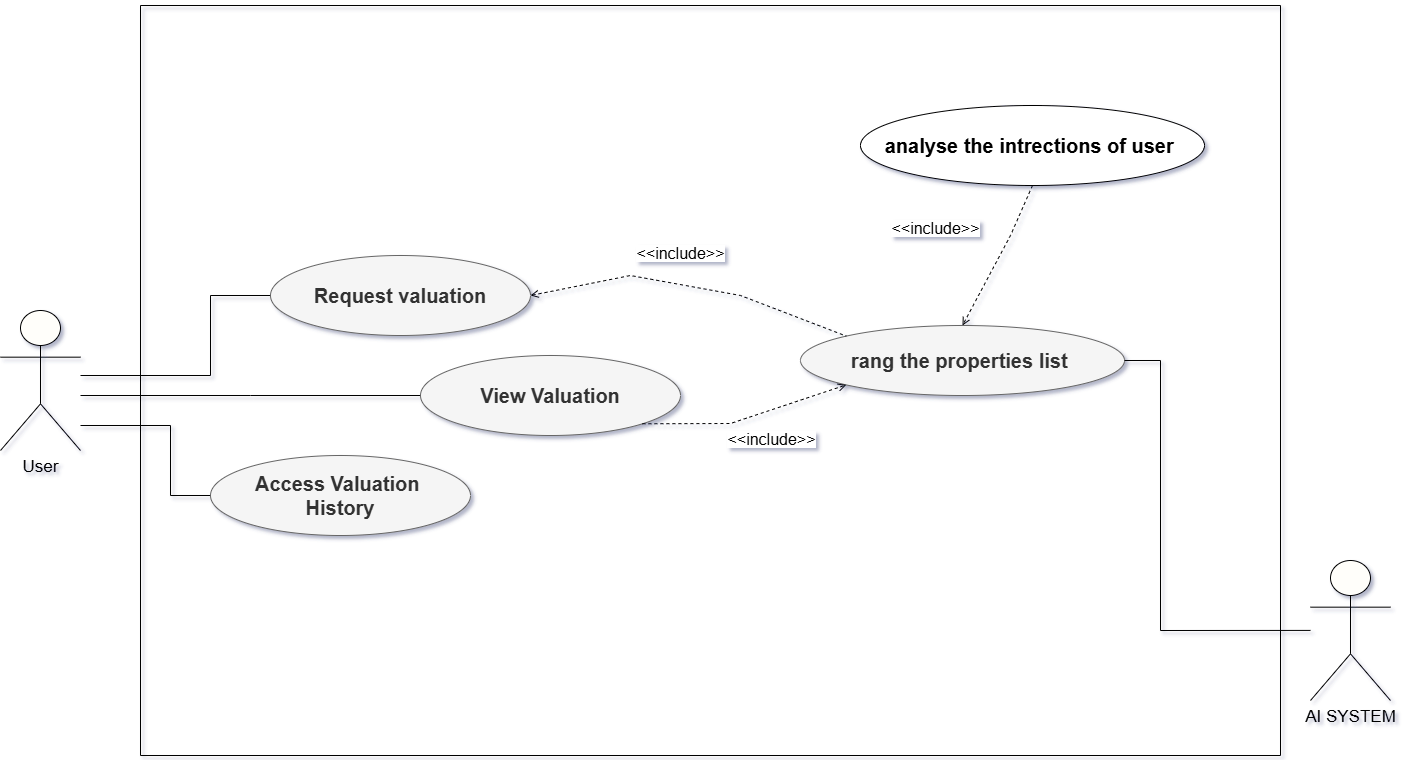
\includegraphics[width=0.8\textwidth]{images/valuation_use_case_diagram.png}
    \caption{Property Valuation Model Use Case Diagram}
    \label{fig:valuation-use-case}
\end{figure}

\subsubsection{Textual Use Case Descriptions}

\textbf{Use Case: Request Property Valuation}
\begin{itemize}
    \item \textbf{Actor}: User (representing Super Admin, Admin, Real Estate Agent)
    \item \textbf{Precondition}: User is authenticated and has access to valuation features
    \item \textbf{Main Flow}: 
    \begin{enumerate}
        \item User inputs property details (location, size, type, amenities)
        \item System validates input data
        \item System processes data through ML model
        \item System returns market value and rental income predictions
        \item User reviews and saves valuation results
    \end{enumerate}
    \item \textbf{Alternative Flow}: If data is incomplete, system requests additional information
    \item \textbf{Postcondition}: Valuation is stored and available for future reference
\end{itemize}

\subsection{System Design}
\subsubsection{Class Diagram}
The property valuation system follows object-oriented design principles. Figure \ref{fig:valuation-class-diagram} shows the main classes and their relationships.
\newpage

\begin{figure}[htbp]
    \centering
    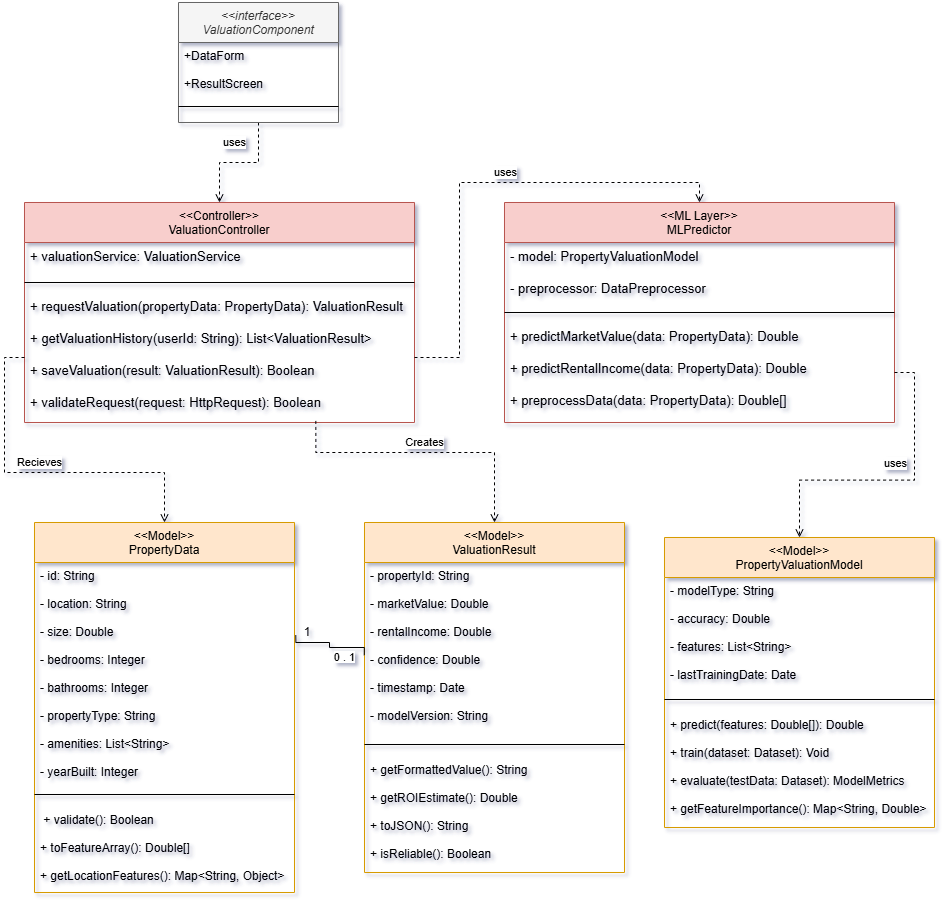
\includegraphics[width=0.9\textwidth]{images/valuation_class_diagram.png}
    \caption{Property Valuation Model Class Diagram}
    \label{fig:valuation-class-diagram}
\end{figure}
\subsection{Model Architecture and Training Process}
\subsubsection{Data Features for Valuation}
The accuracy of the property valuation model heavily relies on the quality and comprehensiveness of the input data. Figure \ref{fig:geo-propriety-data} outlines the key geo-property data features utilized by the model. These features capture essential characteristics of a property and its location, enabling the model to learn complex relationships and predict market values and rental incomes effectively.
\newpage
\begin{figure}[htbp]
    \centering
    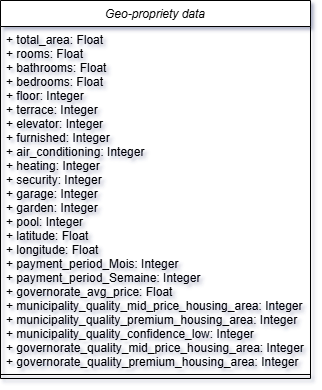
\includegraphics[width=0.4\textwidth]{images/geo-propriety-data.png} % Replace with your actual image path
    \caption{Geo-propriety Data Features for AI Models}
    \label{fig:geo-propriety-data}
\end{figure}

\subsubsection{Model Selection}
To develop an accurate property valuation prediction model, several regression algorithms were evaluated. The following models were selected for training and comparison due to their distinct characteristics and common effectiveness in similar predictive tasks:
\begin{itemize}
    \item \textbf{Linear Regression}: Chosen as a baseline model due to its simplicity and interpretability. It helps in understanding the linear relationships between the features and the target variables (market value and rental income).
    \item \textbf{Random Forest Regressor}: An ensemble learning method that operates by constructing a multitude of decision trees at training time. It is robust to overfitting, handles non-linear relationships well, and often provides high accuracy.
    \item \textbf{Gradient Boosting Regressor}: Another powerful ensemble technique that builds models in a stage-wise fashion. It is known for its high predictive accuracy and ability to optimize for various loss functions, making it suitable for complex regression tasks.
\end{itemize}
These models were trained on the prepared dataset, and their performances were evaluated to select the most suitable one for deployment in the Korpor platform.

\subsubsection{Feature Importance Analysis}
Understanding which features contribute most to the model's predictions is crucial for model interpretability and refinement. After training the selected model, a feature importance analysis was conducted. Figure \ref{fig:feature-importance} displays the top 15 most important features identified by the model. This analysis helps in validating the model's logic.
\newpage

\begin{figure}[htbp]
    \centering
    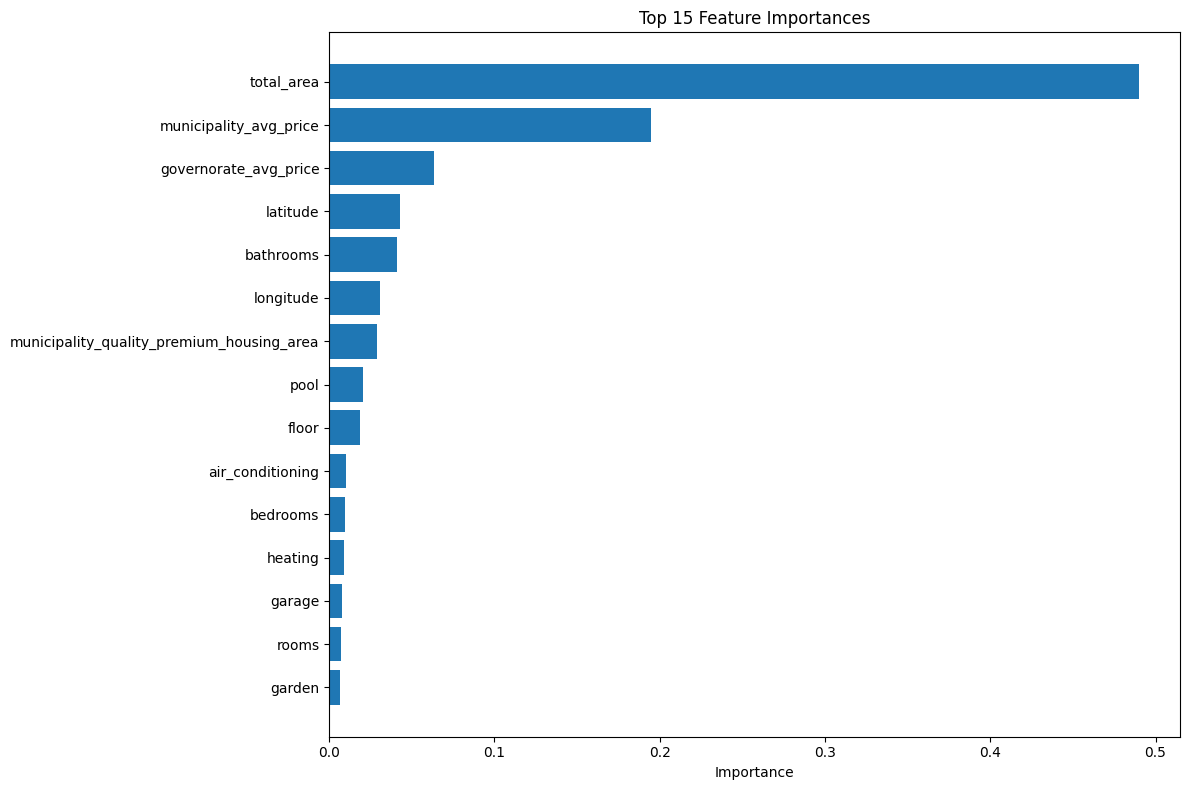
\includegraphics[width=0.8\textwidth]{images/top_15_feature_importance.png} % Assuming image is in 'images' directory
    \caption{Top 15 Feature Importance for Property Valuation Model}
    \label{fig:feature-importance}
\end{figure}

\subsubsection{Model Evaluation and Metrics}
The performance of the trained regression models was rigorously evaluated using standard metrics to ensure reliability and accuracy. Key metrics such as Mean Absolute Error (MAE), Mean Squared Error (MSE), Root Mean Squared Error (RMSE), and R-squared (R²) score were computed on a held-out test dataset. Figure \ref{fig:model-test-metrics} presents a summary of these performance metrics for the chosen valuation model. These results provide a quantitative assessment of the model's ability to generalize to unseen data.


\begin{figure}[htbp]
    \centering
    \begin{minipage}{0.48\textwidth}
        \centering
        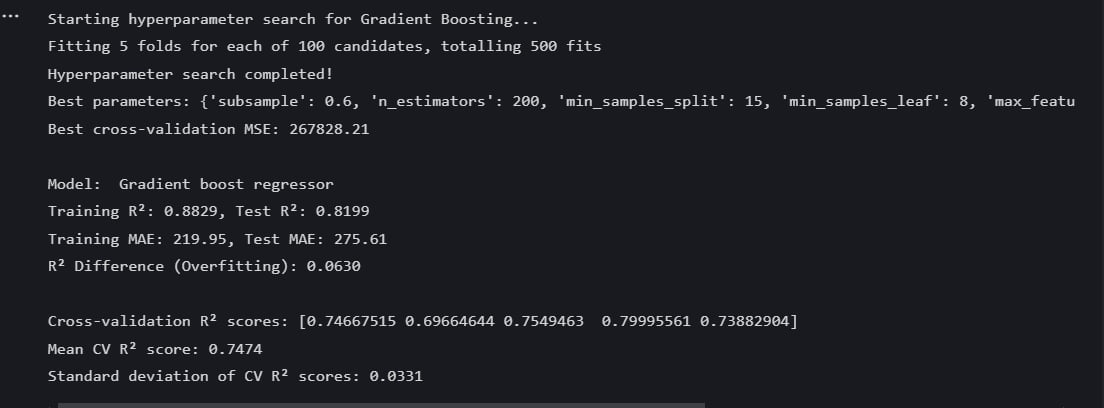
\includegraphics[width=\linewidth]{images/apartmenet location.jpeg}
        \caption*{Apartment Location Prediction}
    \end{minipage}
    \hfill
    \begin{minipage}{0.48\textwidth}
        \centering
        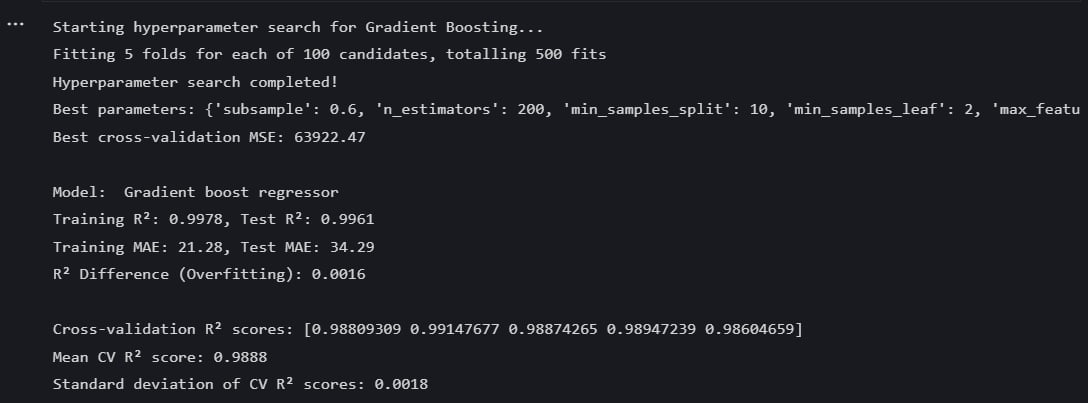
\includegraphics[width=\linewidth]{images/maison location.jpeg}
        \caption*{House Location Prediction}
    \end{minipage}
    
    \vspace{0.5cm}
    
    \begin{minipage}{0.48\textwidth}
        \centering
        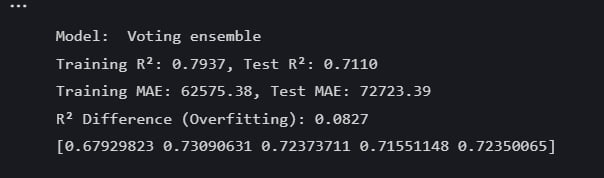
\includegraphics[width=\linewidth]{images/apartmeent vente.jpeg}
        \caption*{Apartment Sale Prediction}
    \end{minipage}
    \hfill
    \begin{minipage}{0.48\textwidth}
        \centering
        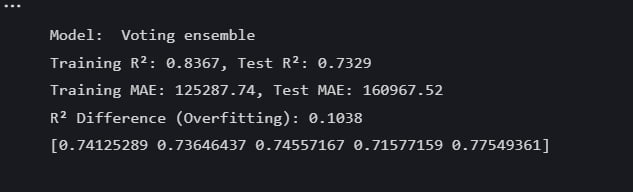
\includegraphics[width=\linewidth]{images/maison vente.jpeg}
        \caption*{House Sale Prediction}
    \end{minipage}
    
    \caption{Prediction Model Test Metrics Summary}
    \label{fig:model-test-metrics}
\end{figure}
\newpage

\subsubsection{Prediction Sequence Flow}
The interaction sequence for the AI property valuation prediction model in Figure \ref{fig:ai-prediction-sequence}.

\begin{figure}[htbp]
    \centering
    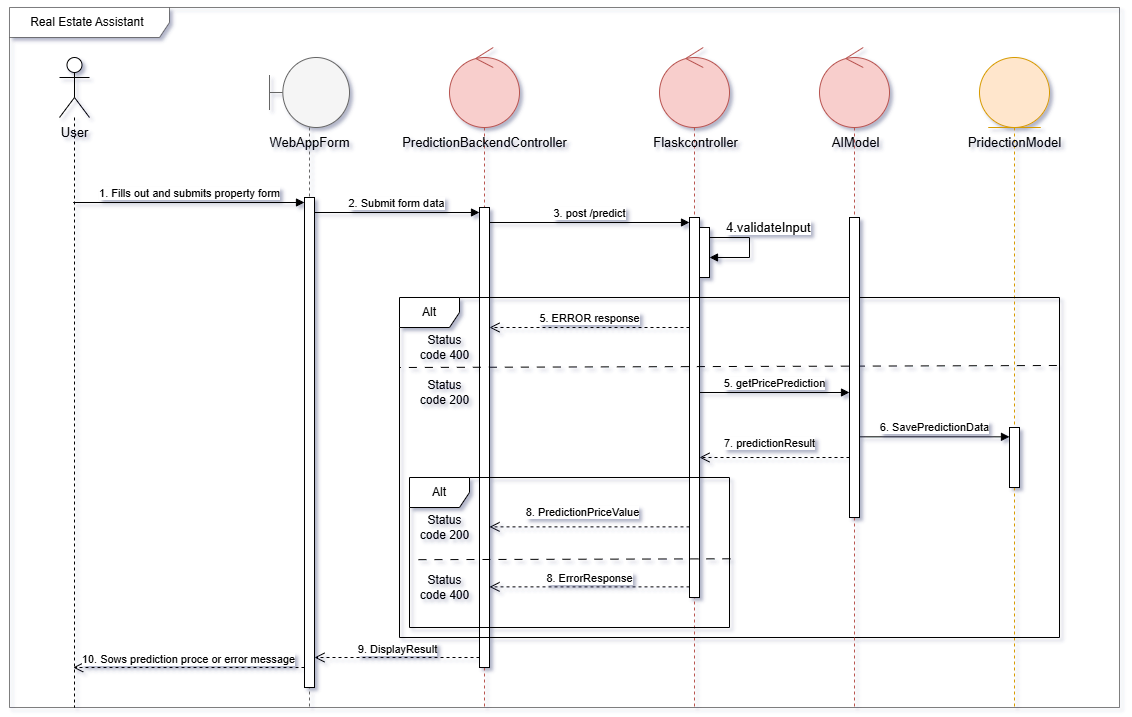
\includegraphics[width=1\textwidth]{images/sequence_AI_prediction_model.png} % Assuming image is in 'images' directory
    \caption{AI Property Valuation Prediction Sequence Diagram}
    \label{fig:ai-prediction-sequence}
\end{figure}


\subsubsection{Prediction User Interface}
Figure \ref{fig:prediction-form} shows the input form, and Figure \ref{fig:prediction-results} displays an example of the prediction results screen.

\begin{figure}[htbp]
        \centering
        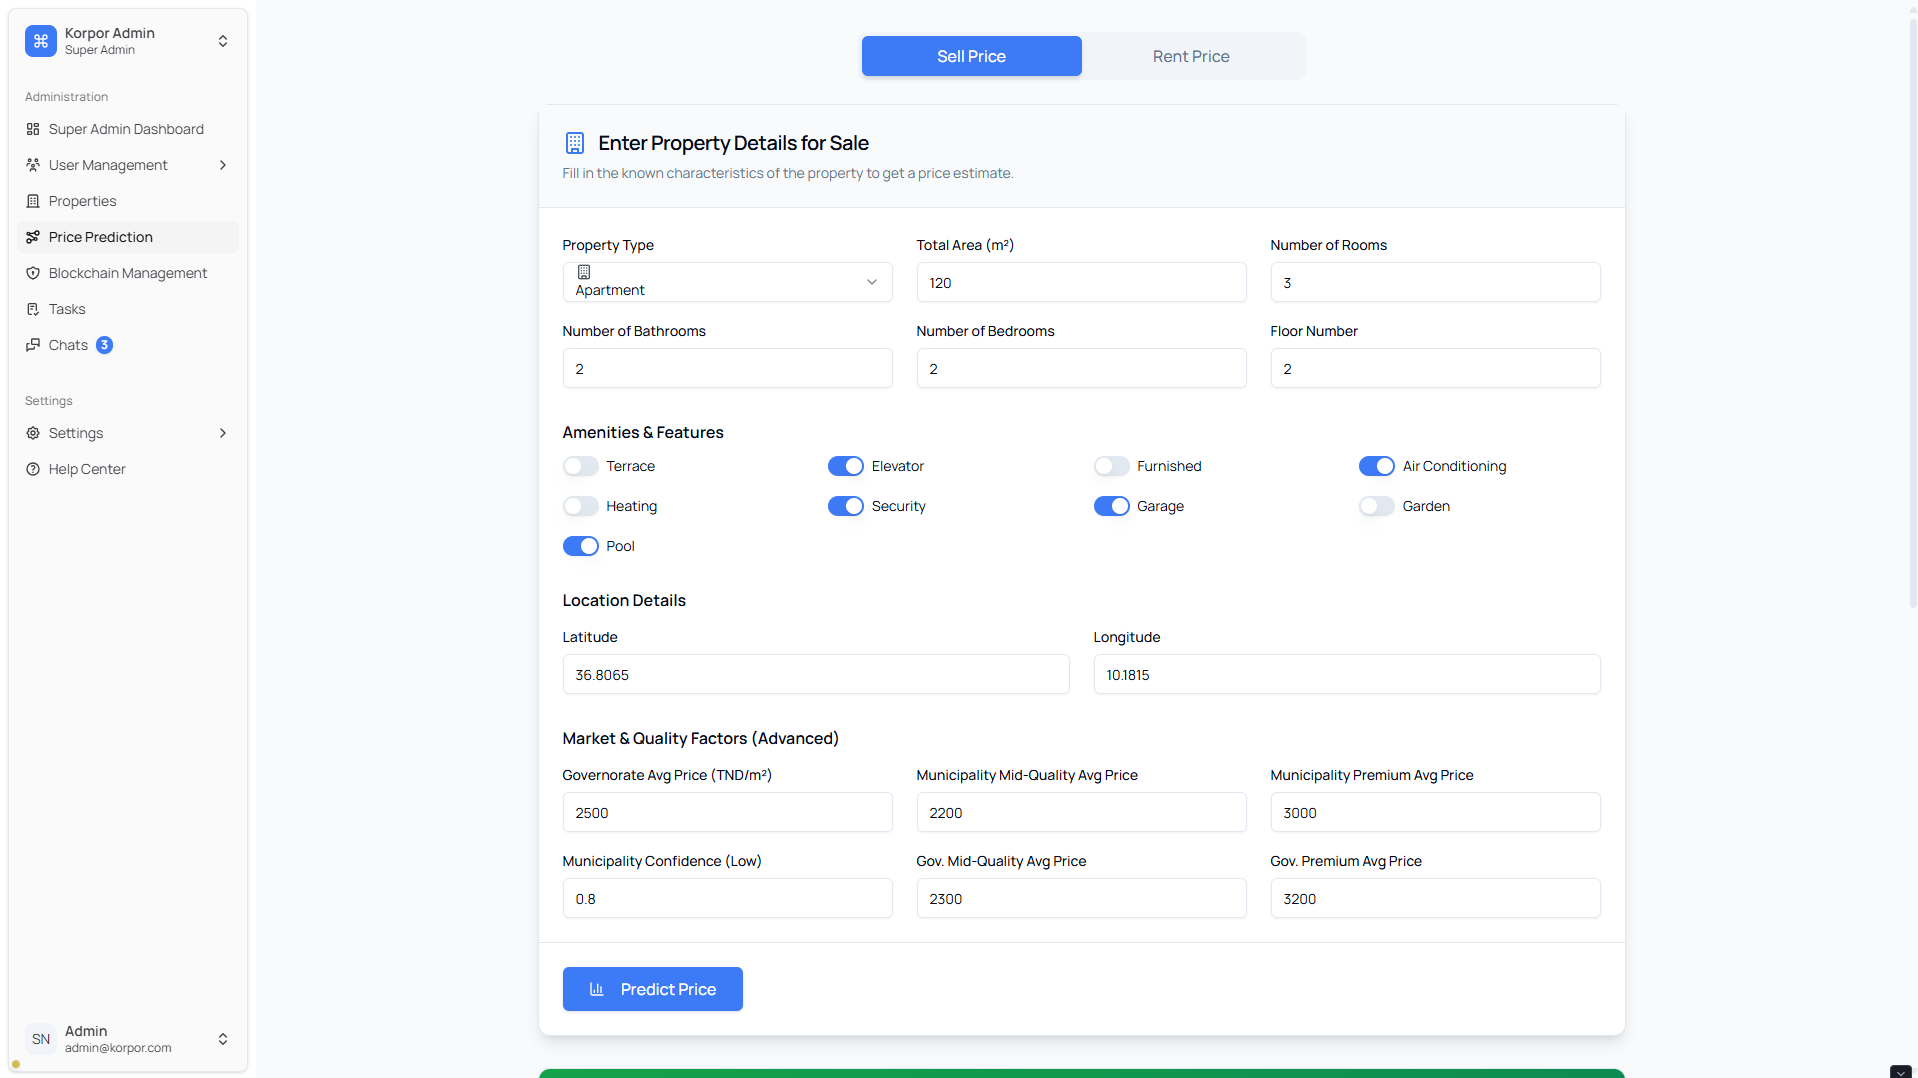
\includegraphics[width=0.7\textwidth]{images/screenshot_form_predition.png}
        \caption{Property Details Input Form for Valuation}
        \label{fig:prediction-form}
\end{figure}

\newpage
\begin{figure}[htbp]
        \centering
        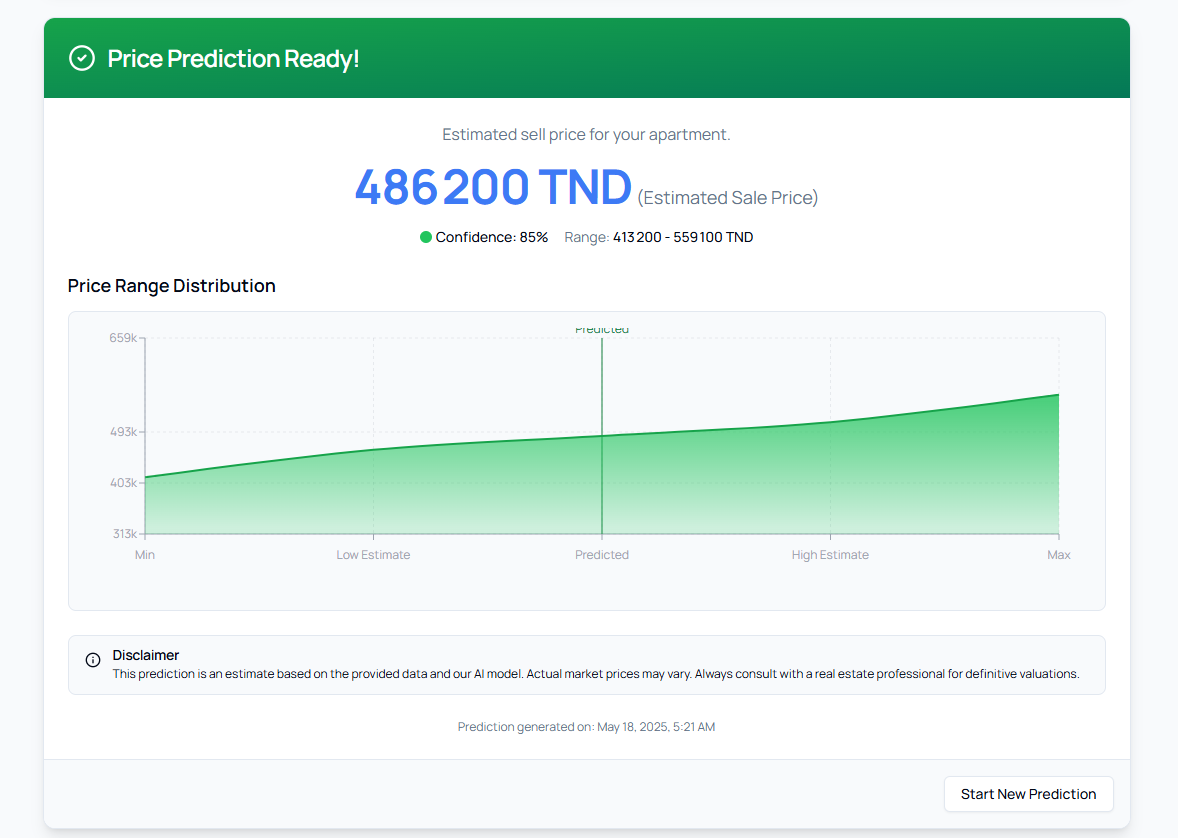
\includegraphics[width=0.7\textwidth]{images/screenshot_predctionscreen.png}
        \caption{Valuation Prediction Results Screen}
        \label{fig:prediction-results}
\end{figure}

\subsubsection{Mobile Investment Insights}
The Korpor mobile application provides investors with direct access to AI-powered property valuations, including future evaluation insights generated by the prediction model. This feature empowers users to make data-driven investment decisions by visualizing potential growth and returns. Figure \ref{fig:mobile-future-evaluation} showcases the mobile interface where these future evaluations are presented to the investor.

\begin{figure}[htbp]
    \centering
    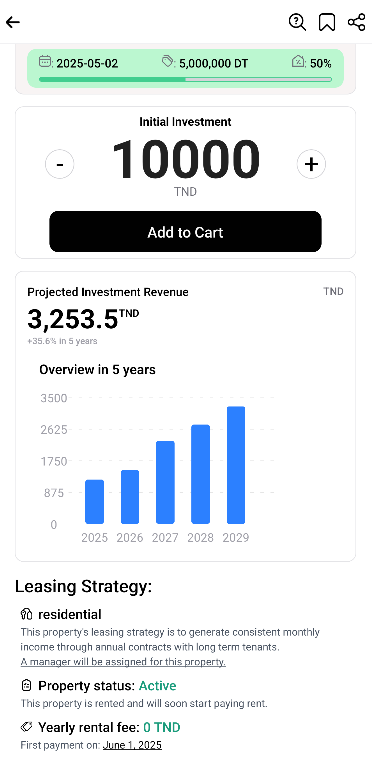
\includegraphics[width=0.3\textwidth]{images/mobile_future_evaluation.png} % Replace with your actual image path
    \caption{Mobile Interface for Future Property Evaluation Insights}
    \label{fig:mobile-future-evaluation}
\end{figure}


\subsubsection{Mobile Interface Testing (Maestro)}
To ensure a seamless and reliable user experience on the mobile platform, the interface for displaying AI-driven property evaluations underwent end-to-end testing using Maestro. The tests covered user flows for accessing predictions and interacting with the displayed data. Figure \ref{fig:maestro-tests-mobile} shows the successful completion of these Maestro tests, validating the robustness of the mobile UI components related to the AI features.

\begin{figure}[htbp]
    \centering
    % \includegraphics[width=0.8\textwidth]{images/maestro_test_mobile_passed.png} % Replace with your actual image path
    \caption{Maestro Test Results for Mobile Prediction Interface}
    \label{fig:maestro-tests-mobile}
\end{figure}

% \begin{table}[htbp]
%     \centering
%     \begin{tabular}{|c|l|l|l|c|}
%         \hline
%         \textbf{Test ID} & \textbf{Scenario} & \textbf{Input} & \textbf{Expected Output} & \textbf{Status} \\
%         \hline
%         VAL-001 & Valid property data & Complete property details & Accurate valuation & \checkmark \\
%         \hline
%         VAL-002 & Incomplete data & Missing property size & Error message & \checkmark \\
%         \hline
%         VAL-003 & Edge case location & Remote area property & Reasonable estimate & \checkmark \\
%         \hline
%         VAL-004 & High-value property & Luxury property details & Premium valuation & \checkmark \\
%         \hline
%         VAL-005 & Model performance & Large dataset & MAE < 10\% & \checkmark \\
%         \hline
%     \end{tabular}
%     \caption{Property Valuation Model Test Scenarios}
%     \label{tab:valuation-test-scenarios}
% \end{table}

\newpage

\section{Sprint 4: Real Estate Assistant (NLP Chatbot)}
\subsection*{Overview}
The Real Estate Assistant is an intelligent NLP-powered chatbot designed to provide investors with instant access to real estate legal information and guidance. This AI assistant helps users understand complex legal concepts, property regulations, and investment procedures through natural language conversations.

\subsection{Requirements Analysis}
\subsubsection{Use Case Diagram}
The Real Estate Assistant serves primarily investors who need legal guidance during their property investment journey. Figure \ref{fig:assistant-use-case} illustrates the main use cases for the AI assistant.
\newpage
\begin{figure}[htbp]
    \centering
    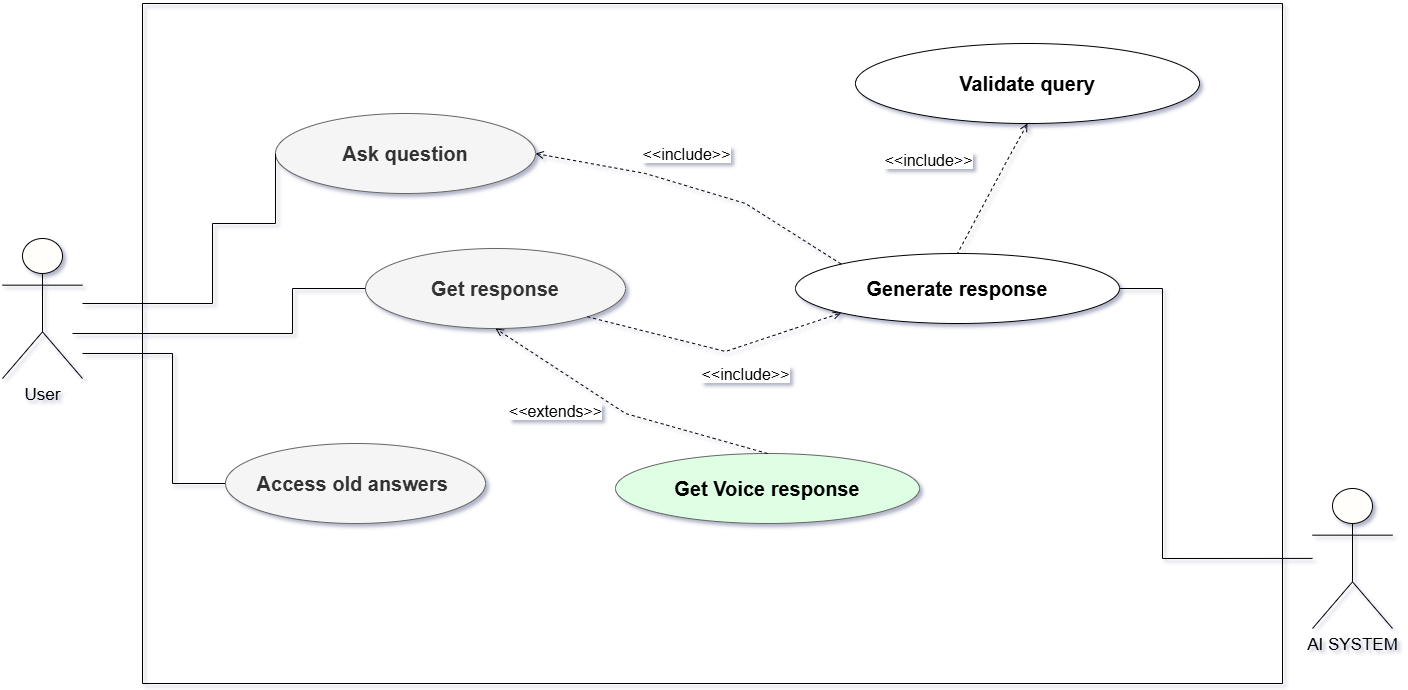
\includegraphics[width=0.9\textwidth]{images/assistant_use_case_diagram.png}
    \caption{Real Estate Assistant Use Case Diagram}
    \label{fig:assistant-use-case}
\end{figure}

\subsubsection{Textual Use Case Descriptions}

\textbf{Use Case: Ask Legal Question}
\begin{itemize}
    \item \textbf{Actor}: Investor
    \item \textbf{Precondition}: User is authenticated and has access to the mobile app
    \item \textbf{Main Flow}: 
    \begin{enumerate}
        \item Investor opens chat interface
        \item Investor types legal question in natural language
        \item System processes question using NLP
        \item System retrieves relevant legal information
        \item System provides comprehensive answer with references
        \item System maintains conversation context for follow-up questions
    \end{enumerate}
    \item \textbf{Alternative Flow}: If question is unclear, system asks for clarification
    \item \textbf{Postcondition}: Conversation is saved for future reference
\end{itemize}

\textbf{Use Case: Provide Legal Guidance}
\begin{itemize}
    \item \textbf{Actor}: System (AI Assistant)
    \item \textbf{Precondition}: User has asked a legal question
    \item \textbf{Main Flow}: 
    \begin{enumerate}
        \item System analyzes question intent and entities
        \item System searches legal knowledge base
        \item System generates contextual response
        \item System provides relevant legal references
        \item System suggests related topics
    \end{enumerate}
    \item \textbf{Postcondition}: User receives accurate legal information
\end{itemize}

\subsection{System Design}
\subsubsection{Class Diagram}
The Real Estate Assistant follows a modular architecture for NLP processing and knowledge management. Figure \ref{fig:assistant-class-diagram} shows the main classes and their relationships.

\begin{figure}[htbp]
    \centering
    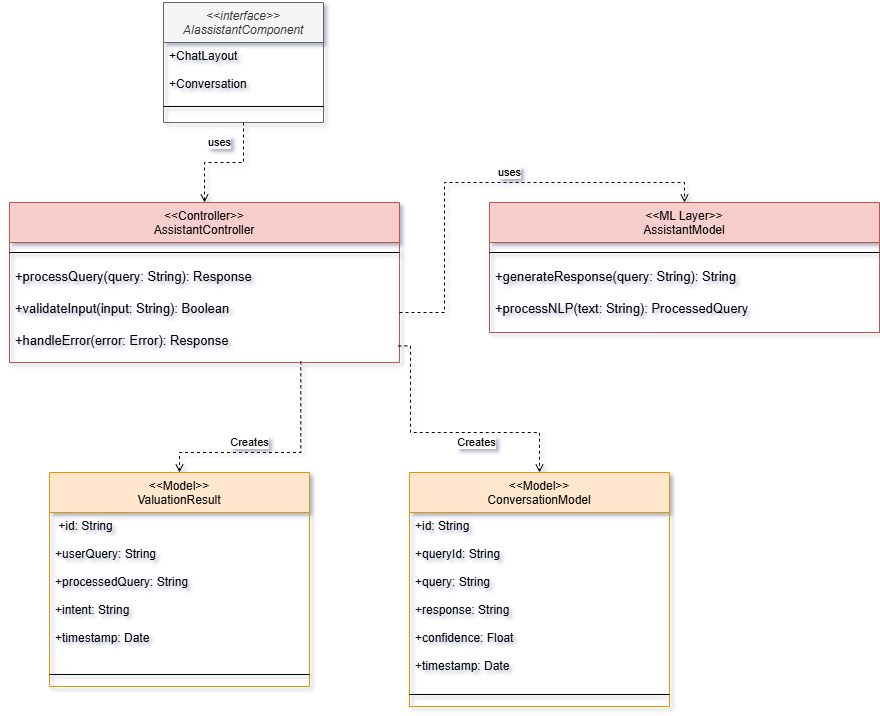
\includegraphics[width=0.8\textwidth]{images/assistant_class_diagram.png}
    \caption{Real Estate Assistant Class Diagram}
    \label{fig:assistant-class-diagram}
\end{figure}

\subsubsection{Sequence Diagram (MVC)}
The interaction flow between the mobile interface, backend services, and NLP processing components is illustrated in Figure \ref{fig:assistant-sequence-mvc}.
\newpage
\begin{figure}[htbp]
    \centering
    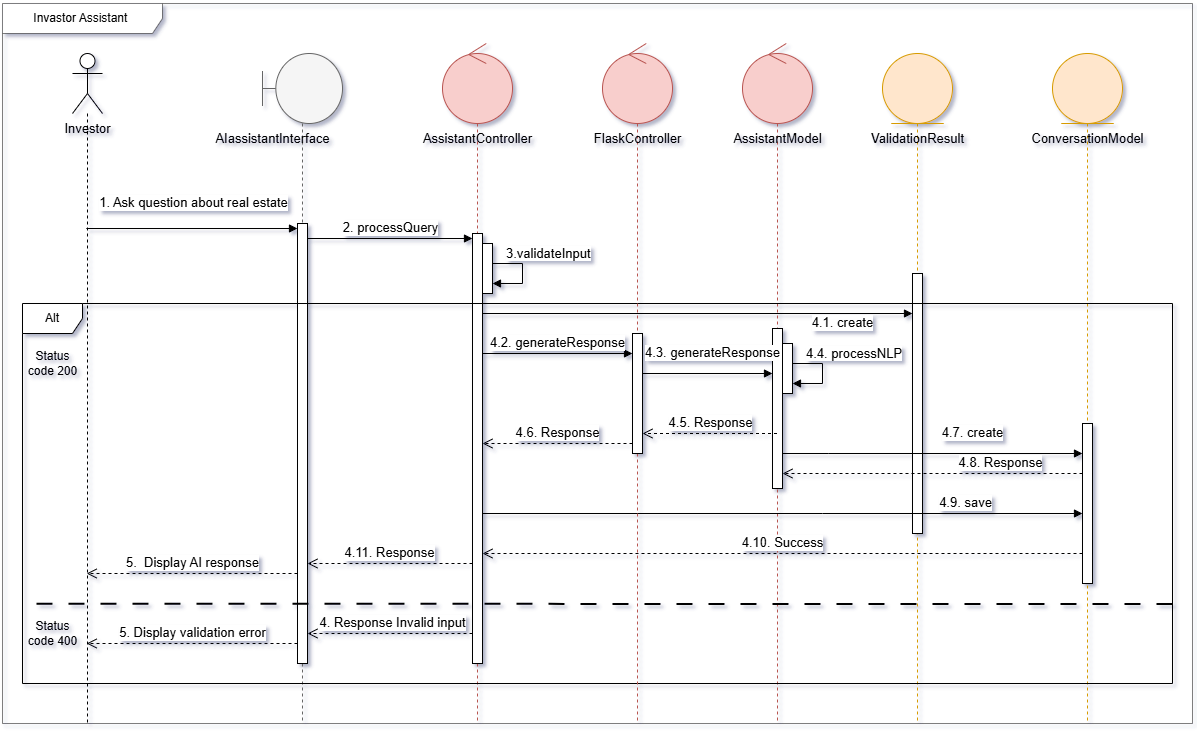
\includegraphics[width=1\textwidth]{images/assistant_sequence_mvc.png}
    \caption{Real Estate Assistant MVC Sequence Diagram}
    \label{fig:assistant-sequence-mvc}
\end{figure}

\subsection{Implementation}
\subsubsection{NLP Model Architecture}
The Real Estate Assistant utilizes advanced natural language processing techniques to understand and respond to user queries. The system employs:

\begin{itemize}
    \item \textbf{Intent Recognition}: Identifies the purpose of user questions (property law, taxes, contracts, etc.)
    \item \textbf{Entity Extraction}: Extracts key information like property types, locations, and legal concepts
    \item \textbf{Context Management}: Maintains conversation history for coherent multi-turn dialogues
    \item \textbf{Response Generation}: Creates natural, informative responses based on legal knowledge base
\end{itemize}

\subsubsection{Legal Knowledge Base}
The assistant's knowledge base contains comprehensive information about:
\begin{itemize}
    \item Tunisian real estate law and regulations
    \item Property investment procedures
    \item Tax implications and calculations
    \item Contract templates and requirements
    \item Common legal issues and solutions
\end{itemize}

\subsubsection{Chat Interface Implementation}
The mobile chat interface provides an intuitive way for investors to interact with the AI assistant. Figure \ref{fig:assistant-mobile-chat} shows the chat interface design.

\begin{figure}[htbp]
    \centering
    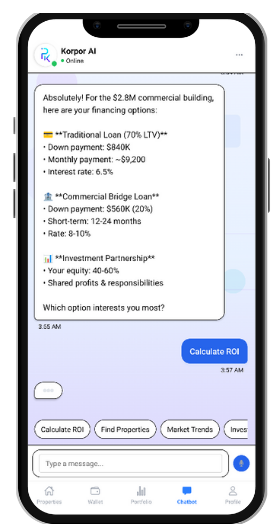
\includegraphics[width=0.3\textwidth]{images/assistant_mobile_chat.png}
    \caption{Mobile Chat Interface for Real Estate Assistant}
    \label{fig:assistant-mobile-chat}
\end{figure}


\subsection{Testing and Validation}
\subsubsection{Test Scenarios}
The Real Estate Assistant underwent extensive testing to ensure accurate responses and reliable performance. Table \ref{tab:assistant-test-scenarios} presents the key test scenarios.

\begin{table}[htbp]
    \centering
    \begin{tabular}{|c|l|l|l|c|}
        \hline
        \textbf{Scenario} & \textbf{Input} & \textbf{Expected Output} & \textbf{Status} \\
        \hline
         Property tax query & "What are property taxes?" & Detailed tax information & \checkmark \\
        \hline
        Contract question & "What's in a rental contract?" & Contract requirements & \checkmark \\
        \hline
         Investment procedure & "How to buy property?" & Step-by-step guide & \checkmark \\
        \hline
         Legal compliance & "Foreign investment rules?" & Regulatory information & \checkmark \\
        \hline
         Context follow-up & Multi-turn conversation & Coherent responses & \checkmark \\
        \hline
         Unclear question & Ambiguous query & Clarification request & \checkmark \\
        \hline
    \end{tabular}
    \caption{Real Estate Assistant Test Scenarios}
    \label{tab:assistant-test-scenarios}
\end{table}

\newpage

\section{Role-Based Backoffice Agent}
\subsection*{Overview}
The Role-Based Backoffice Agent is an intelligent AI system designed to assist different user roles (Super Admin, Admin, Real Estate Agent) with automated task management, workflow optimization, and decision support. This AI agent adapts its behavior and recommendations based on the specific role and responsibilities of the authenticated user.

\subsection{Requirements Analysis}
\subsubsection{Use Case Diagram}
The Role-Based Backoffice Agent serves multiple user types with role-specific functionalities and automated assistance. Figure \ref{fig:backoffice-use-case} illustrates the main use cases for each role.

\begin{figure}[htbp]
    \centering
    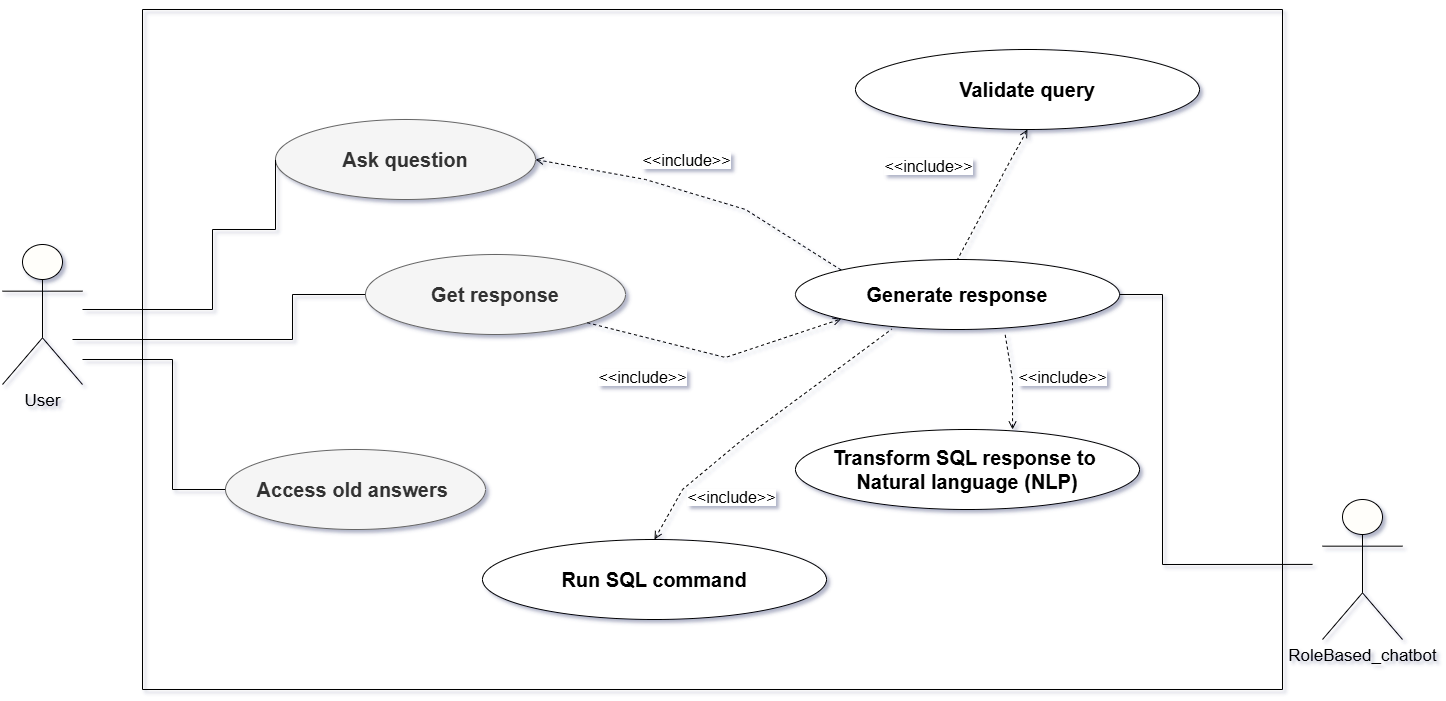
\includegraphics[width=1\textwidth]{images/backoffice_use_case_diagram.png}
    \caption{Role-Based Backoffice Agent Use Case Diagram}
    \label{fig:backoffice-use-case}
\end{figure}

\subsubsection{Textual Use Case Descriptions}

\textbf{Use Case: Automate Task Management}
\begin{itemize}
    \item \textbf{Actor}: User (representing Super Admin, Admin, Real Estate Agent)
    \item \textbf{Precondition}: User is authenticated with specific role permissions
    \item \textbf{Main Flow}: 
    \begin{enumerate}
        \item User accesses backoffice dashboard
        \item System identifies user role and permissions
        \item AI agent analyzes pending tasks and priorities
        \item System suggests automated actions based on role
        \item User approves or modifies suggested actions
        \item System executes approved automated tasks
    \end{enumerate}
    \item \textbf{Alternative Flow}: If automation requires approval, system queues for manual review
    \item \textbf{Postcondition}: Tasks are efficiently managed with minimal manual intervention
\end{itemize}

\textbf{Use Case: Provide Role-Specific Insights}
\begin{itemize}
    \item \textbf{Actor}: AI Agent
    \item \textbf{Precondition}: User has accessed dashboard with specific role
    \item \textbf{Main Flow}: 
    \begin{enumerate}
        \item System analyzes user role and current context
        \item AI generates role-specific insights 
        \item AI suggests optimization opportunities
        \item System provides actionable recommendations
    \end{enumerate}
    \item \textbf{Postcondition}: User receives personalized insights for their role
\end{itemize}

\subsection{System Design}
\subsubsection{Class Diagram}
The Role-Based Backoffice Agent follows a role-based architecture with specialized services for each user type. Figure \ref{fig:backoffice-class-diagram} shows the main classes and their relationships.
\newpage
\begin{figure}[htbp]
    \centering
    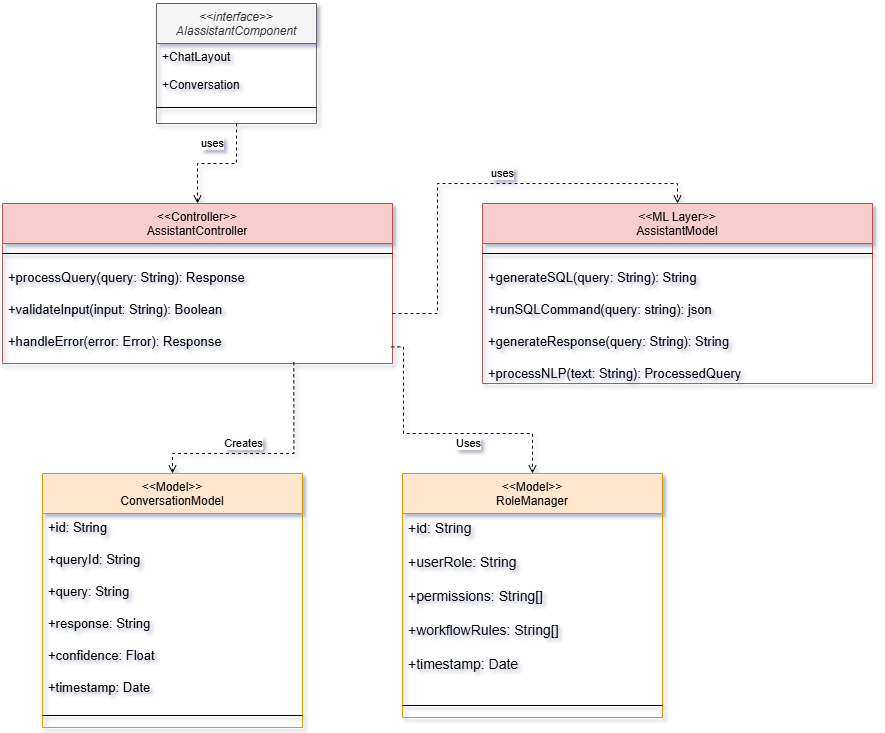
\includegraphics[width=1\textwidth]{images/backoffice_class_diagram.png}
    \caption{Role-Based Backoffice Agent Class Diagram}
    \label{fig:backoffice-class-diagram}
\end{figure}

\subsubsection{Sequence Diagram (MVC)}
The interaction flow between the web interface, role management services, and AI processing components is illustrated in Figure \ref{fig:backoffice-sequence-mvc}.
\newpage
\begin{figure}[htbp]
    \centering
    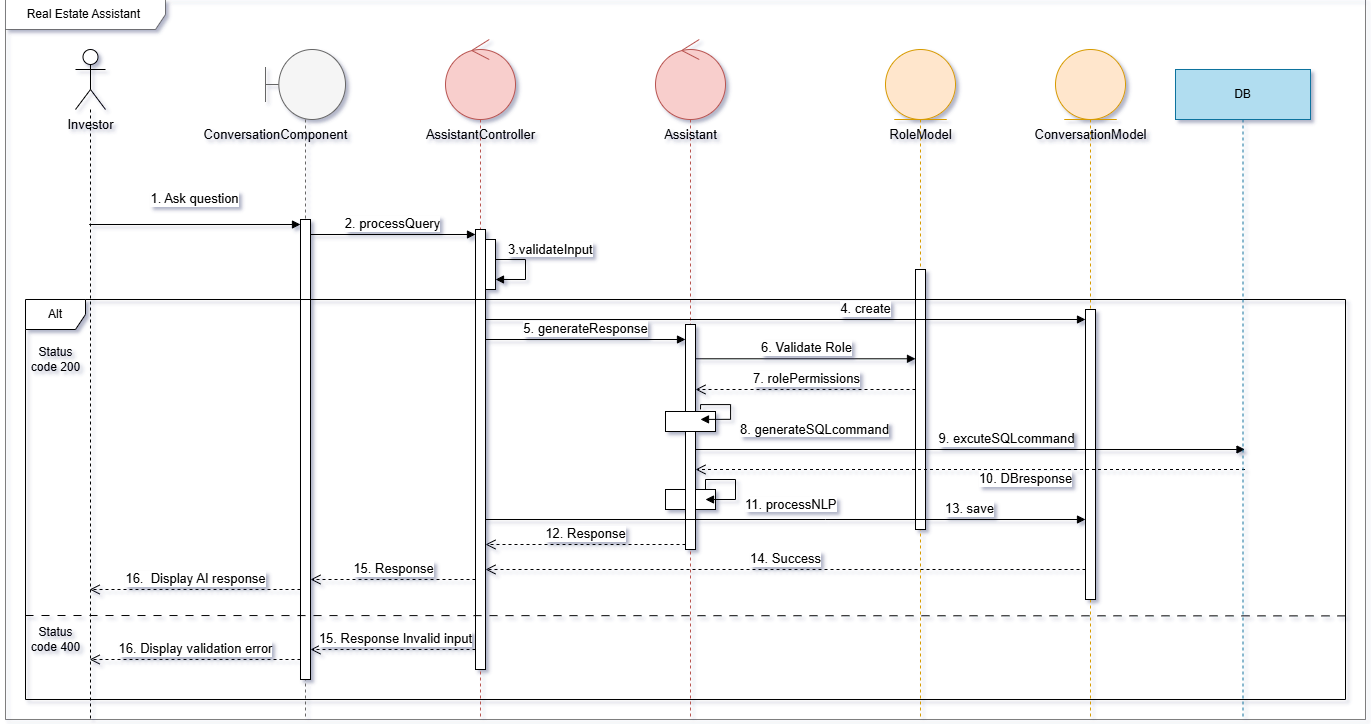
\includegraphics[width=1\textwidth]{images/backoffice_sequence_mvc.png}
    \caption{Role-Based Backoffice Agent MVC Sequence Diagram}
    \label{fig:backoffice-sequence-mvc}
\end{figure}

\subsection{Implementation}
\subsubsection{Role-Based AI Logic}
The Backoffice Agent utilizes sophisticated role-based AI algorithms to provide personalized assistance:

\begin{itemize}
    \item \textbf{Super Admin Features}: System monitoring, user management, platform analytics, security oversight
    \item \textbf{Admin Features}: Property management, user support, content moderation, performance tracking
    \item \textbf{Real Estate Agent Features}: Client management, property listings, sales tracking, commission calculations
\end{itemize}

\subsubsection{Automated Workflow Management}
The system automates routine tasks based on role permissions:
\begin{itemize}
    \item Property approval workflows for admins
    \item User verification processes for super admins
    \item Client follow-up reminders for agents
    \item Performance report generation for all roles
\end{itemize}

\newpage
\subsubsection{Dashboard Implementation}
Each role receives a customized dashboard with relevant tools and insights. Figure \ref{fig:backoffice-dashboard} shows the role-specific dashboard implementations.

\begin{figure}[htbp]
    \centering
    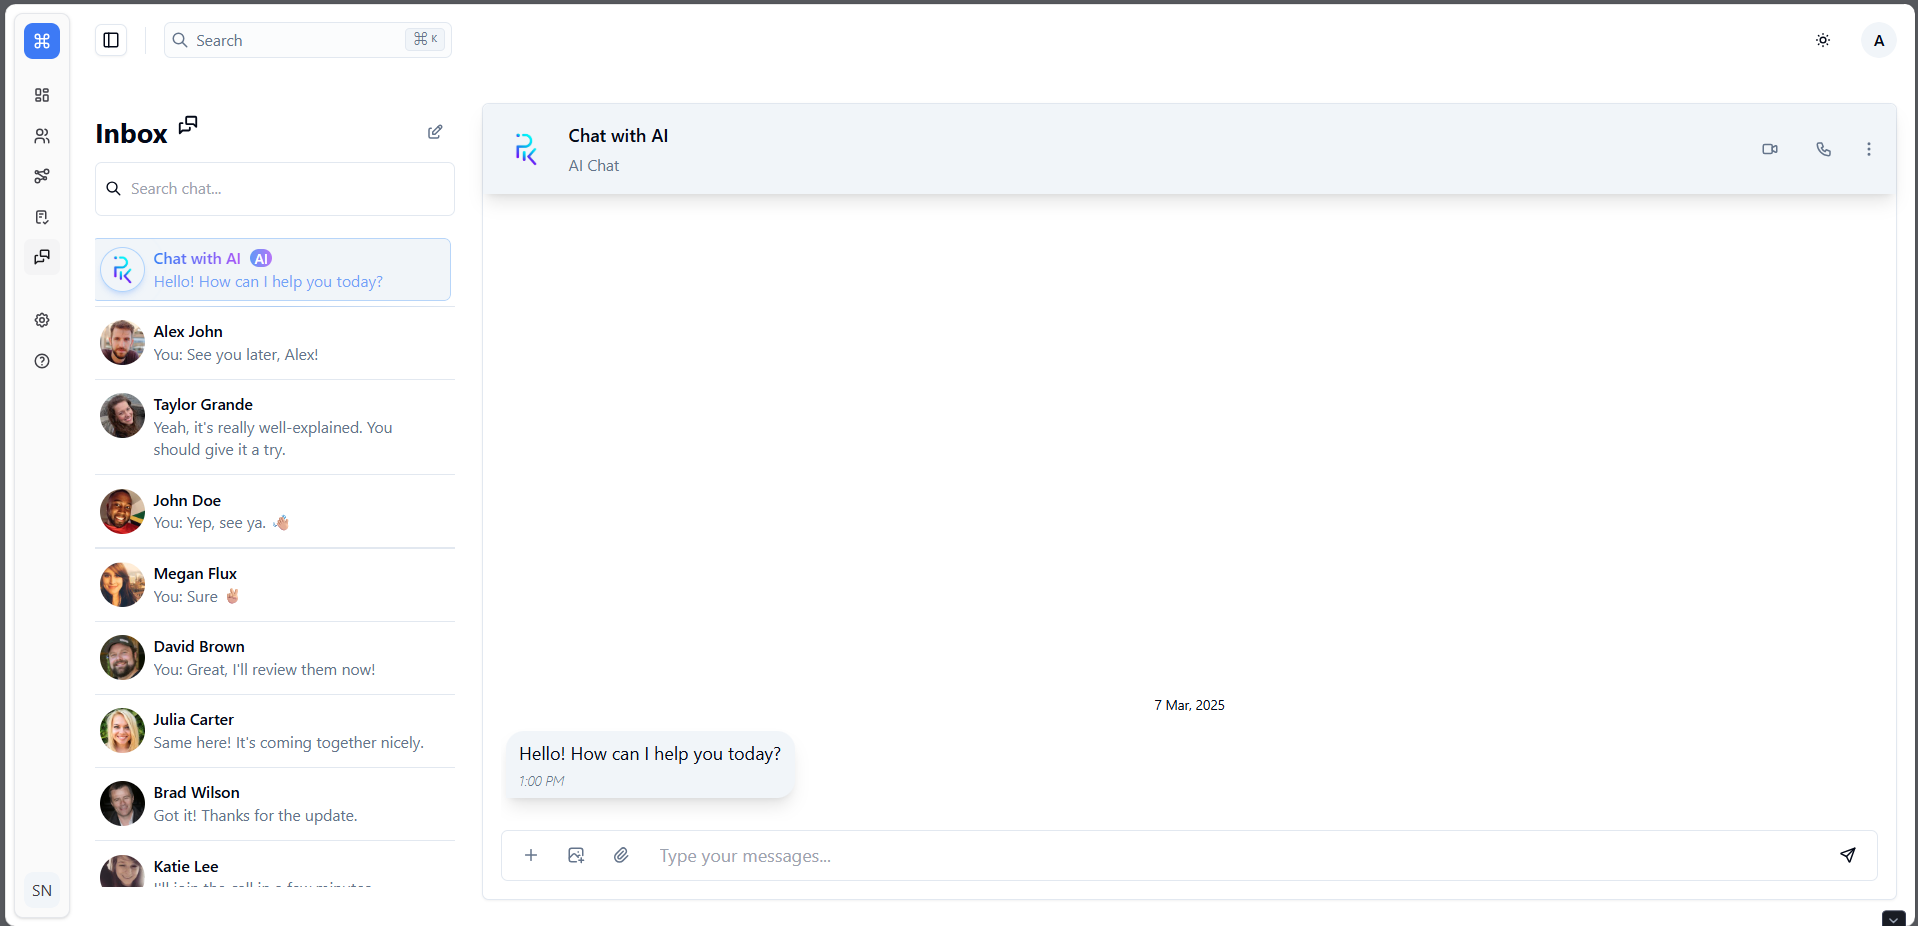
\includegraphics[width=1\textwidth]{images/assistant_web_interface.png}
    \caption{Web Interface for Real Estate Assistant}
    \label{fig:assistant-web-interface}
\end{figure}


\subsection{Testing and Validation}
\subsubsection{Test Scenarios}
The Role-Based Backoffice Agent underwent comprehensive testing across all user roles. Table \ref{tab:backoffice-test-scenarios} presents the key test scenarios.

\begin{table}[htbp]
    \centering
    \begin{tabular}{|c|l|l|l|c|}
        \hline
        \textbf{Scenario} & \textbf{User Role} & \textbf{Expected Output} & \textbf{Status} \\
        \hline
        Role identification & Super Admin & Admin dashboard access & \checkmark \\
        \hline
        Task automation & Admin & Property approval workflow & \checkmark \\
        \hline
        Performance insights & Real Estate Agent & Sales analytics & \checkmark \\
        \hline
        Permission validation & Admin & Restricted super admin features & \checkmark \\
        \hline
        AI recommendations & All roles & Role-specific suggestions & \checkmark \\
        \hline
        Workflow management & Super Admin & System optimization tips & \checkmark \\
        \hline
    \end{tabular}
    \caption{Role-Based Backoffice Agent Test Scenarios}
    \label{tab:backoffice-test-scenarios}
\end{table}
\newpage
\section{Sprint 5: Investor-Focused Recommendation System}
\subsection*{Overview}
The Investor-Focused Recommendation System is an advanced AI model that analyzes investor behavior, preferences, and market conditions to provide personalized property investment recommendations. This system leverages machine learning algorithms to match investors with optimal investment opportunities based on their risk profile, budget, and investment goals.

\begin{figure}[htbp]
    \centering
    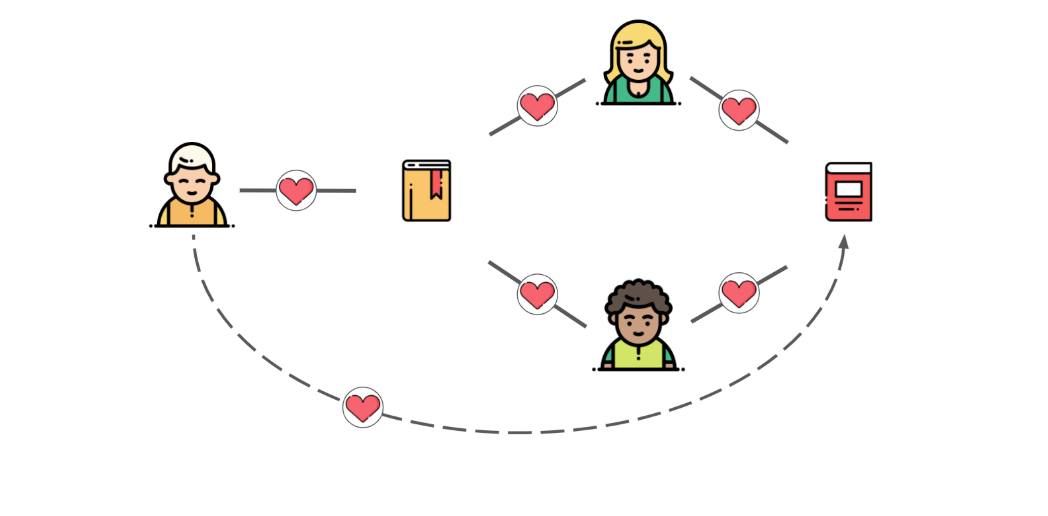
\includegraphics[width=0.7\textwidth]{images/collaborative_filtring.png}
    \caption{Collaborative Filtering Recommendation System Overview}
    \label{fig:collaborative-filtering-overview}
\end{figure}

\subsection{Requirements Analysis}
\subsubsection{Use Case Diagram}
The Recommendation System serves investors by analyzing their profiles and suggesting suitable investment opportunities. Figure \ref{fig:recommendation-use-case} illustrates the main use cases for the recommendation engine.

\begin{figure}[htbp]
    \centering
    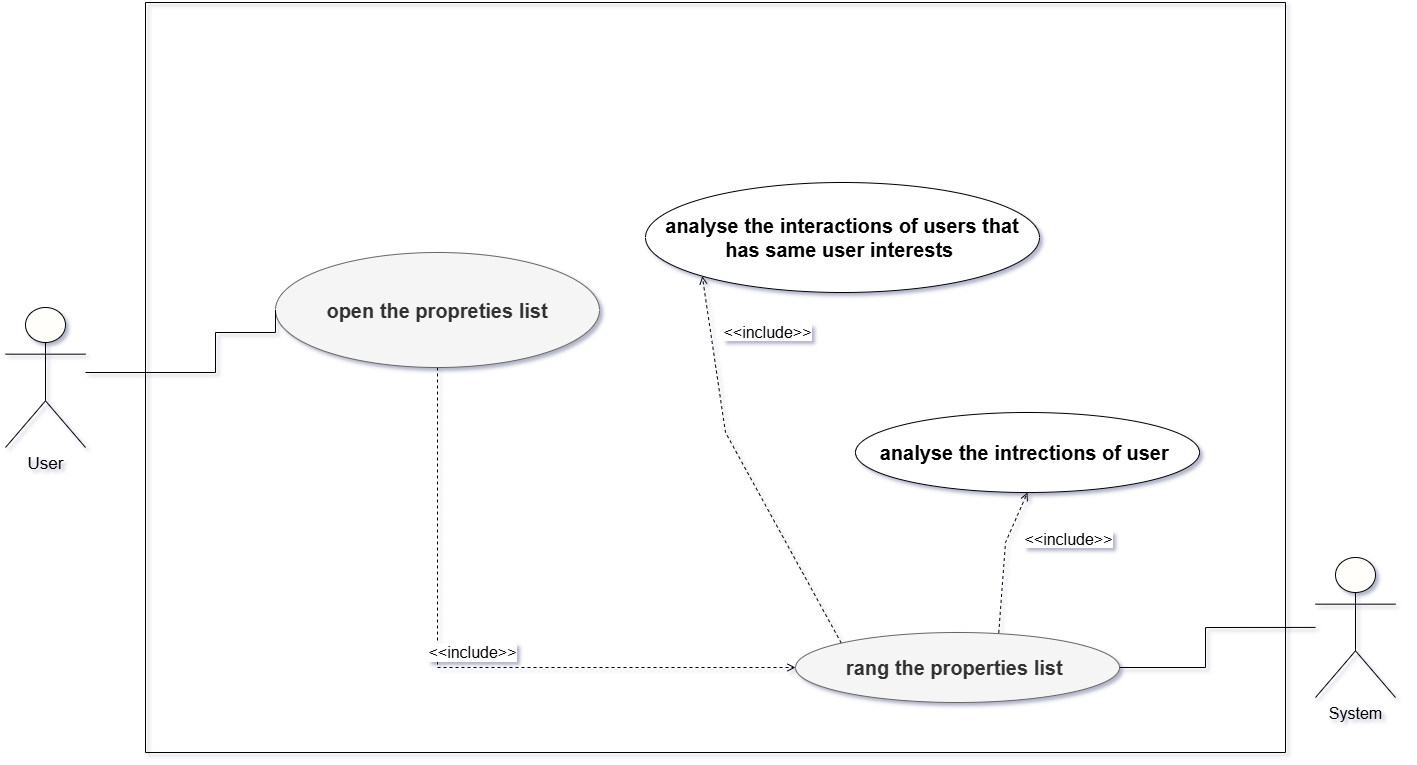
\includegraphics[width=0.7\textwidth]{images/recommendation_use_case_diagram.png}
    \caption{Investor-Focused Recommendation System Use Case Diagram}
    \label{fig:recommendation-use-case}
\end{figure}

\subsubsection{Textual Use Case Descriptions}

\textbf{Use Case: Generate Investment Recommendations}
\begin{itemize}
    \item \textbf{Actor}: User (Investor)
    \item \textbf{Precondition}: Investor has completed profile setup and preferences
    \item \textbf{Main Flow}: 
    \begin{enumerate}
        \item Investor accesses recommendations section
        \item System analyzes investor profile and preferences
        \item AI processes available investment opportunities
        \item System matches properties with investor criteria
        \item AI ranks recommendations by compatibility score
        \item System presents personalized investment suggestions
    \end{enumerate}
    \item \textbf{Alternative Flow}: If no suitable matches, system suggests expanding criteria
    \item \textbf{Postcondition}: Investor receives tailored investment recommendations
\end{itemize}

\textbf{Use Case: Update Investment Preferences}
\begin{itemize}
    \item \textbf{Actor}: Investor
    \item \textbf{Precondition}: Investor is authenticated and has existing profile
    \item \textbf{Main Flow}: 
    \begin{enumerate}
        \item Investor accesses preference settings
        \item User modifies risk tolerance, budget, or location preferences
        \item System validates and saves updated preferences
        \item AI recalculates recommendation algorithms
        \item System generates new recommendations based on updated profile
    \end{enumerate}
    \item \textbf{Postcondition}: Recommendations are updated to reflect new preferences
\end{itemize}

\subsection{System Design}
\subsubsection{Class Diagram}
The Recommendation System uses collaborative filtering and content-based algorithms for personalized suggestions. Figure \ref{fig:recommendation-class-diagram} shows the main classes and their relationships.

\begin{figure}[htbp]
    \centering
    % \includegraphics[width=0.8\textwidth]{images/recommendation_class_diagram.png}
    \caption{Investor-Focused Recommendation System Class Diagram}
    \label{fig:recommendation-class-diagram}
\end{figure}

\subsubsection{Sequence Diagram (MVC)}
The interaction flow between the mobile interface, recommendation engine, and machine learning components is illustrated in Figure \ref{fig:recommendation-sequence-mvc}.

\begin{figure}[htbp]
    \centering
    % \includegraphics[width=1\textwidth]{images/recommendation_sequence_mvc.png}
    \caption{Recommendation System MVC Sequence Diagram}
    \label{fig:recommendation-sequence-mvc}
\end{figure}

\subsection{Implementation}
\subsubsection{Machine Learning Algorithms}
The Recommendation System employs multiple ML techniques for optimal suggestions:

\begin{itemize}
    \item \textbf{Collaborative Filtering}: Analyzes similar investor behaviors and preferences
    \item \textbf{Content-Based Filtering}: Matches properties based on investor criteria
    \item \textbf{Hybrid Approach}: Combines multiple algorithms for enhanced accuracy
    \item \textbf{Deep Learning}: Neural networks for complex pattern recognition
\end{itemize}

\subsubsection{Investor Profiling}
The system creates comprehensive investor profiles including:
\begin{itemize}
    \item Risk tolerance assessment
    \item Investment budget and timeline
    \item Geographic preferences
    \item Property type preferences
    \item Previous investment history
    \item Market behavior analysis
\end{itemize}

\subsubsection{Mobile Recommendations Interface}
The mobile app provides an intuitive interface for viewing personalized recommendations. Figure \ref{fig:recommendation-mobile} shows the mobile recommendation implementation.

\begin{figure}[htbp]
    \centering
    \includegraphics[width=0.3\textwidth]{images/recommendation_mobile.png}
    \caption{Mobile Interface for Investment Recommendations}
    \label{fig:recommendation-mobile}
\end{figure}

\subsubsection{Recommendation Algorithm Visualization}
The system provides transparency in recommendation logic through visual explanations. Figure \ref{fig:recommendation-algorithm} demonstrates how recommendations are generated and explained to users.

\begin{figure}[htbp]
    \centering
    % \includegraphics[width=0.8\textwidth]{images/recommendation_algorithm.png}
    \caption{Recommendation Algorithm Visualization}
    \label{fig:recommendation-algorithm}
\end{figure}

\subsubsection{Personalized Dashboard}
Investors receive a personalized dashboard with recommendations and portfolio insights. Figure \ref{fig:recommendation-dashboard} shows the recommendation dashboard design.


\subsection{Testing and Validation}
\subsubsection{Test Scenarios}
The Recommendation System underwent extensive testing to ensure accuracy and relevance. Table \ref{tab:recommendation-test-scenarios} presents the key test scenarios.

\begin{table}[htbp]
    \centering
    \begin{tabular}{|c|l|l|l|c|}
        \hline
        \textbf{Scenario} & \textbf{Input} & \textbf{Expected Output} & \textbf{Status} \\
        \hline
        New investor profile & Basic preferences & Relevant recommendations & \checkmark \\
        \hline
        Preference update & Changed risk tolerance & Updated suggestions & \checkmark \\
        \hline
        Budget constraint & Limited budget & Affordable options & \checkmark \\
        \hline
         Location preference & Specific city & Local properties & \checkmark \\
        \hline
        Algorithm accuracy & Historical data & High precision score & \checkmark \\
        \hline
        Performance optimization & Large dataset & Fast response time & \checkmark \\
        \hline
    \end{tabular}
    \caption{Recommendation System Test Scenarios}
    \label{tab:recommendation-test-scenarios}
\end{table}


\subsubsection{Mobile App Testing (Maestro)}
The mobile recommendation interface underwent thorough testing using Maestro to ensure optimal user experience. Figure \ref{fig:maestro-recommendation} shows the successful test execution.

\begin{figure}[htbp]
    \centering
    % \includegraphics[width=0.8\textwidth]{images/maestro_recommendation_tests.png}
    \caption{Maestro Test Results for Recommendation System}
    \label{fig:maestro-recommendation}
\end{figure}






\cleardoublepage

% Chapter 5:
\chapter{Blockchain}

\section*{Introduction}

In recent years, blockchain technology has emerged as a powerful tool for building trust, enhancing transparency, and decentralizing processes across various industries \cite{Nakamoto2008Bitcoin, Tapscott2016Blockchain}. In the context of Korpor, a platform aimed at facilitating real estate investments, blockchain plays a crucial role in ensuring the reliability and traceability of financial operations.

Traditional real estate investment systems often rely on centralized authorities and intermediaries, which may introduce delays, additional costs, or even fraudulent behavior. By integrating blockchain, Korpor addresses these limitations by recording key transactions such as investments, rent distributions, and project creation directly on a decentralized ledger \cite{Veuger2018RealEstateBlockchain}. This ensures that all stakeholders can verify actions in a transparent and immutable manner, without needing to trust a single party.

Moreover, smart contracts enable the automation of operations like rent distribution and investment validation, reducing human error and increasing efficiency \cite{Buterin2014Ethereum, Szabo1997SmartContracts}.

\section{Overview of Use Cases}

The blockchain integration within the \textbf{\textcolor{primary}{Korpor}} platform addresses several core functionalities that benefit from decentralization and transparency. The main use cases implemented include:

\begin{itemize}
    \item \textbf{Investment Recording}
    \begin{itemize}
        \item Immutable proof of ownership for the investor.
        \item Transparent public records of all investment flows.
        \item Verifiable data for audits or external reviews.
    \end{itemize}

    \item \textbf{Project Registration}
    \begin{itemize}
        \item Proof of project existence on-chain.
        \item Traceability of project updates and funding status.
        \item Protection against unauthorized modifications.
    \end{itemize}

    \item \textbf{Rent Distribution}
    \begin{itemize}
        \item Calculate and distribute rental income fairly to investors.
        \item Automate distribution without manual intervention.
        \item Log each rent payout on the blockchain for transparency.
    \end{itemize}

    \item \textbf{Transaction Verification}
    \begin{itemize}
        \item Trust in the platform.
        \item User empowerment to track their funds and participation.
        \item Regulatory compliance through transparent financial trails.
    \end{itemize}
\end{itemize}

\section{Objectives of Blockchain Integration}

The integration of blockchain technology into the \textbf{\textcolor{primary}{Korpor}} platform serves several key objectives aimed at enhancing the system's reliability, transparency, and automation capabilities:

\begin{itemize}
    \item \textbf{Security and trust in transactions}
    \begin{itemize}
        \item Ensures that each transaction is securely signed and verified.
        \item Builds trust among users by preventing unauthorized modifications \cite{Zheng2018BlockchainChallenges}.
        \item Enhances transparency through verifiable on-chain records.
    \end{itemize}

    \item \textbf{Decentralization and immutability}
    \begin{itemize}
        \item Eliminates single points of failure by distributing data across the blockchain.
        \item Guarantees that data, once written, cannot be altered \cite{Antonopoulos2018MasteringEthereum}.
        \item Promotes resilience and long-term reliability of the system.
    \end{itemize}

    \item \textbf{Automation through smart contracts}
    \begin{itemize}
        \item Enables automatic execution of business logic (e.g., rent distribution) \cite{Bartoletti2017EmpiricalAnalysis}.
        \item Reduces manual intervention and human error.
        \item Increases system efficiency through self-executing contracts.
    \end{itemize}
\end{itemize}

\section{Technical Architecture}

The blockchain component is designed to integrate seamlessly within the overall architecture of the \textbf{\textcolor{primary}{Korpor}} platform. This section outlines how the blockchain fits into the system and the technologies used for its implementation.

\begin{itemize}
    \item \textbf{How blockchain fits into the overall system architecture}
    \begin{itemize}
        \item The backend communicates with smart contracts deployed on the Ethereum blockchain.
        \item Transactions such as investments, project registrations, and rent distributions are processed and recorded on-chain.
        \item The blockchain acts as a complementary layer to ensure data integrity and traceability.
    \end{itemize}

    \item \textbf{On-chain vs off-chain components}
    \begin{itemize}
        \item \textit{On-chain:}
        \begin{itemize}
            \item Smart contracts handle investments, project registrations, and rent distributions.
            \item Data recorded on-chain is immutable and publicly verifiable.
        \end{itemize}
        \item \textit{Off-chain:}
        \begin{itemize}
            \item User data, authentication, and detailed analytics are managed by the backend and stored in a centralized database (MySQL).
            \item Interaction with the blockchain is facilitated through API endpoints and external services \cite{Xu2019ArchitectingBlockchainApplications}.
        \end{itemize}
    \end{itemize}

    \item \textbf{Technologies used}
   \begin{itemize}
    \item \includegraphics[width=0.05\textwidth]{images/icons/solidity.png} \textbf{Solidity:} A high-level programming language specifically designed for writing secure, efficient, and decentralized smart contracts on the Ethereum blockchain \cite{SolidityDocs}.
    
    \item \includegraphics[width=0.05\textwidth]{images/icons/etherscan.png} \textbf{Ethers.js:} A popular JavaScript library used to interact with the Ethereum blockchain, providing functionality to manage accounts, send transactions, and call smart contract functions \cite{EthersJSDocs}.
    
    \item \includegraphics[width=0.05\textwidth]{images/icons/sepolia.png} \textbf{Sepolia Testnet:} A test network for Ethereum that allows developers to deploy and test their smart contracts in a safe, controlled environment without spending real cryptocurrency.
    
    \item \includegraphics[width=0.05\textwidth]{images/icons/infura.png} \textbf{Infura:} A cloud-based platform that provides access to Ethereum nodes via JSON-RPC, eliminating the need to run a full Ethereum node \cite{InfuraWeb3}.
    
    \item \includegraphics[width=0.05\textwidth]{images/icons/metamask.png} \textbf{MetaMask:} A widely-used browser extension and mobile application that serves as a cryptocurrency wallet for interacting with decentralized applications \cite{MetaMaskDocs}.
   \end{itemize}
\end{itemize}

\subsection{Third-Party Payment Integration: Paymee}

In the Korpor platform, secure and reliable payment processing is fundamental to enabling users to invest in real estate projects with confidence. While blockchain handles transparency and decentralization for on-chain interactions, fiat payments from users need to be handled via trusted third-party providers. For this purpose, we chose \textbf{Paymee} as our main payment gateway.

% Placeholder for Paymee Framework diagram
\begin{figure}[htbp]
\centering
% PLACEHOLDER: Insert Paymee Framework diagram here
\includegraphics[width=0.8\textwidth]{images/paymee_framework.png}
\caption{Paymee Framework}
\label{fig:paymee-framework}
\end{figure}

\subsubsection{Role of Paymee in the Architecture}

Paymee acts as a bridge between the user's traditional banking system and our decentralized investment platform. When a user decides to invest in a project, the fiat transaction is processed securely via Paymee. Upon confirmation, the platform triggers an on-chain event that records the investment using a smart contract, ensuring both real-world and blockchain-level consistency.

\begin{itemize}
    \item Paymee provides a secure and verified method for processing payments via bank cards or wallets.
    \item It offers real-time transaction status updates, which are essential for synchronizing with blockchain confirmations.
    \item The integration ensures that only successful payments are recorded on-chain, reducing fraud and improving traceability \cite{Bamakan2020BlockchainPayment}.
\end{itemize}

\subsubsection{Justifying the Choice of Paymee}

Several third-party payment providers are available in Tunisia, including  \textbf{Flouci} \includegraphics[width=0.05\textwidth]{images/icons/flouci_icon.png} and  \textbf{Konnect} \includegraphics[width=0.05\textwidth]{images/icons/konnect_icon.png} , however, \textbf{Paymee} was chosen due to its distinct advantages in several key areas:

\begin{itemize}
  \item \textbf{Regulatory Compliance:} Fully compliant with local regulations and has established partnerships with most major Tunisian banks.
  
  \item \textbf{Developer Experience:} Offers clear documentation, a stable sandbox environment, and responsive customer support.
  
  \item \textbf{Payment Mode:} Supports a wide range of payment methods, including both local and international options.
  
  \item \textbf{Pricing:} Offers simplified and transparent pricing with competitive rates.
  
  \item \textbf{User Experience:} Provides a minimalistic and intuitive user interface that reduces drop-off rates during transactions.
  
  \item \textbf{Flexibility:} Highly flexible and easily integrates into diverse use cases, adapting to the needs of individual investors.
\end{itemize}
\newpage
% Placeholder for Payment Providers Comparison Table
\begin{table}[htbp]
\centering
\caption{Comparison of Payment Providers: Paymee vs Flouci vs Konnect}
\label{tab:payment_comparison}
\begin{tabular}{|p{4cm}|p{3.5cm}|p{3.5cm}|p{3.5cm}|}
\hline
\textbf{Feature} & \textbf{Paymee} & \textbf{Flouci} & \textbf{Konnect} \\ \hline
\textbf{Regulatory Compliance} & Fully compliant with local regulations & Limited compliance & Enterprise-focused, may have specific requirements \\ \hline
\textbf{Developer Experience} & Clear documentation, stable sandbox, responsive support & Less stable APIs, limited documentation & Lengthy onboarding, limited flexibility \\ \hline
\textbf{Payment Model} & Ideal for recurring, high-trust investments & Not suited for investment models & Enterprise-focused with fixed pricing \\ \hline
\textbf{Pricing} & Simplified and transparent & Unclear pricing structure & Complex pricing and fees \\ \hline
\textbf{User Experience} & Minimalistic UI, reliable webhooks, low drop-offs & Less reliable, mobile payment focus & Enterprise UI, longer process, limited customization \\ \hline
\textbf{Flexibility} & High flexibility in fee structures & Low flexibility & Low flexibility, rigid fee structures \\ \hline
\end{tabular}
\end{table}

Based on these factors, \textbf{Paymee} was selected as the most suitable payment provider for the Korpor platform, playing a pivotal role in bridging traditional finance with our blockchain-based investment infrastructure.

\section{Smart Contract Design}

\subsection{Smart Contracts Overview}

A smart contract is a self-executing contract with the terms of the agreement directly written into lines of code \cite{Szabo1997SmartContracts}. These contracts run on blockchain platforms, such as Ethereum, and are designed to automatically enforce and execute the terms of an agreement without the need for intermediaries. 

Smart contracts operate on decentralized networks, ensuring transparency, immutability, and security. They allow parties to interact and transact with one another in a trustless environment, where the contract's logic is executed automatically when predefined conditions are met \cite{Wohrer2018SmartContractApplications}.

\subsection{Smart Contract Responsibilities}

The smart contract in the Korpor application is responsible for managing the critical aspects of the platform. The main responsibilities include:

\begin{itemize}
    \item \textbf{Recording Investments:} The smart contract records each user's investment when they invest in a project.
    \item \textbf{Project Registration:} Real estate companies can register new projects.
    \item \textbf{Rent Distribution:} The contract ensures that rental income is distributed fairly to investors.
    \item \textbf{Transaction Verification:} All actions taken within the contract are securely logged on the blockchain.
\end{itemize}

\subsection{Data Structures and Functions}

In the smart contract, several data structures and functions are employed to manage and store key information, facilitating efficient interaction with the system \cite{Dannen2017SoliditySmartContracts}.

\subsubsection{Data Structures}

The contract uses `structs` to represent complex data types like project and investor details.

\paragraph{Project Struct:}
The `Project` struct stores the details of each project:
\begin{verbatim}
struct Project {
    uint256 projectId;
    string projectName;
    address companyAddress;
    uint256 totalFunding;
    uint256 rentIncome;
    uint256 numInvestors;
}
\end{verbatim}

\paragraph{Investor Struct:}
The `Investor` struct holds information about each investor's investment:
\begin{verbatim}
struct Investor {
    address investorAddress;
    uint256 amountInvested;
    bool hasReceivedRent;
}
\end{verbatim}

\subsubsection{Core Functions}

Several key functions implement the core logic of the platform:

\paragraph{recordInvestment:}
\begin{verbatim}
function recordInvestment(uint256 projectId) public payable {
    require(msg.value > 0, "Investment amount must be greater than zero.");
    projects[projectId].totalFunding += msg.value;
    investments[msg.sender] += msg.value;
    projects[projectId].numInvestors++;
}
\end{verbatim}

\paragraph{recordProject:}
\begin{verbatim}
function recordProject(string memory name, address company) public {
    uint256 projectId = projectCounter++;
    projects[projectId] = Project(projectId, name, company, 0, 0, 0);
}
\end{verbatim}

\paragraph{distributeRent:}
\begin{verbatim}
function distributeRent(uint256 projectId) public {
    uint256 rentAmount = projects[projectId].rentIncome / projects[projectId].numInvestors;
    for (uint256 i = 0; i < projects[projectId].numInvestors; i++) {
        address investor = projects[projectId].investors[i].investorAddress;
        payable(investor).transfer(rentAmount);
        projects[projectId].investors[i].hasReceivedRent = true;
    }
}
\end{verbatim}

\paragraph{getInvestmentDetails:}
\begin{verbatim}
function getInvestmentDetails(address investor) public view returns (uint256) {
    return investments[investor];
}
\end{verbatim}

\subsection{Deployment \& Testing}

\subsubsection{Deployment}

The smart contracts were deployed following a structured workflow \cite{Wust2018BlockchainNeed}:

\begin{itemize}
    \item Compiled and deployed using \includegraphics[width=0.05\textwidth]{images/icons/remix.png} \texttt{Remix IDE} onto the \textbf{Sepolia Testnet}
    \item Deployment transactions signed through \includegraphics[width=0.05\textwidth]{images/icons/metamask.png} \texttt{MetaMask} with test ETH
    \item Contracts made publicly accessible on \includegraphics[width=0.05\textwidth]{images/icons/etherscan.png} \texttt{Etherscan} for validation and transparency
    \item Deployed contract addresses:
    \begin{itemize}
        \item \textbf{Investment Contract:} \texttt{0xC25E147316c1dBD16f5B6427e381f9F4fF9510D6}
        \item \textbf{Projects Contract:} \texttt{0xed3c0f14c4b767A65955B71dD1f8328f51f38DE0}
        \item \textbf{Rent Distribution Contract:} \texttt{0x74Ca4D7B2856dddCb1a074A9e40A7fC33deD6437}
    \end{itemize}
\end{itemize}

\newpage
% Placeholder for Etherscan screenshot after deployment
\begin{figure}[htbp]
  \centering
  % PLACEHOLDER: Insert Etherscan screenshot here
  \includegraphics[width=0.8\textwidth]{images/etherscan_screenshot.png}
  \caption{Investment Contract in Etherscan after deployment}
  \label{fig:etherscan-screenshot}
\end{figure}

\subsubsection{Testing}

The testing process used the following tools:

\begin{itemize}
    \item \includegraphics[width=0.05\textwidth]{images/icons/remix.png} \textbf{Remix IDE:} For writing, testing, and deploying Ethereum smart contracts
    \item \includegraphics[width=0.05\textwidth]{images/icons/hardhat.png} \textbf{Hardhat:} For local blockchain simulation, testing, and deploying contracts
\end{itemize}

The testing approach included:

\begin{itemize}
    \item \textbf{Unit Testing:} Testing core functions individually
    \item \textbf{Integration Testing:} Validating full transaction flows
    \item \textbf{Event Listening:} Capturing and validating event emissions
    \item \textbf{Performance Testing:} Ensuring efficient operation under load \cite{Parizi2018SmartContractProgramming}
\end{itemize}

\newpage
% Placeholder for Smart Contract Deployment & Interaction flowchart
\begin{figure}[htbp]
  \centering
  % PLACEHOLDER: Insert Smart Contract Deployment & Interaction flowchart here
  \includegraphics[width=0.8\textwidth]{images/contract_flowchart.png}
  \caption{Flowchart: Smart Contract Deployment \& Interaction}
  \label{fig:contract-flowchart}
\end{figure}

\newpage
% Placeholder for Full Blockchain Deployment Diagram
% \begin{figure}[htbp]
%   \centering
%   % PLACEHOLDER: Insert Full Blockchain Deployment Diagram here
%   \includegraphics[width=\textwidth]{images/blockchain_deployment_diagram.png}
%   \caption{Full Blockchain Deployment Diagram}
%   \label{fig:blockchain-deployment}
% \end{figure}

\section{Integration Flow}

The integration flow can be summarized as follows \cite{Casino2019BlockchainApplications}:

\subsection{Investment Flow}

\begin{itemize}
    \item The frontend initiates a payment session via Paymee's API
    \item Paymee redirects the user to complete the payment
    \item Upon success, Paymee calls back our backend with the transaction details
    \item After verification, the backend invokes the appropriate smart contract to log the investment on the blockchain
\end{itemize}

% Placeholder for Investment sequence diagram
\begin{figure}[htbp]
  \centering
  % PLACEHOLDER: Insert Investment sequence diagram here
  \includegraphics[width=\textwidth]{images/investment_sequence.png}
  \caption{Sequence Diagram of the Investment Process}
  \label{fig:investment-sequence}
\end{figure}

\subsection{Rent Distribution Flow}

\begin{itemize}
    \item The backend initiates the rent distribution process by invoking the smart contract
    \item The smart contract calculates each investor's share based on their investment proportion
    \item For each investor, the smart contract emits an event indicating the calculated share
    \item The backend listens for these events, verifies the data, and triggers the payment through Paymee's API
    \item System records are updated after successful transactions
\end{itemize}

% Placeholder for Rent distribution sequence diagram
\begin{figure}[htbp]
  \centering
  % PLACEHOLDER: Insert Rent distribution sequence diagram here
  \includegraphics[width=\textwidth]{images/rent_distribution_sequence.png}
  \caption{Sequence Diagram of Rent Distribution}
  \label{fig:rent-distribution-sequence}
\end{figure}

\section{Backoffice Features}

\subsection{Administrative Dashboard}

The backoffice provides administrators with a comprehensive dashboard to manage the platform. Key features include:

\begin{itemize}
    \item Real-time monitoring of blockchain transactions
    \item Project management interface for adding, editing, and removing properties
    \item User management with role-based access control \cite{Botha2021BackofficeBlockchain}
    \item Financial reporting and analytics
    \item Blockchain transaction verification tools
\end{itemize}

% Placeholder for Admin Dashboard screenshot
\begin{figure}[htbp]
  \centering
  % PLACEHOLDER: Insert Admin Dashboard screenshot here
%   \includegraphics[width=0.9\textwidth]{images/admin_dashboard.png}
  \caption{Blockchain Transaction Monitoring in Administrative Dashboard}
  \label{fig:admin-dashboard}
\end{figure}

\subsection{Transaction Management}

Administrators can monitor and manage all types of transactions:

\begin{itemize}
    \item View all investment records with blockchain verification links
    \item Monitor rent distribution status and history
    \item Verify payment processing through the Paymee integration
    \item Generate financial reports and audit trails
\end{itemize}

% Placeholder for Transaction Management Interface
\begin{figure}[htbp]
  \centering
  % PLACEHOLDER: Insert Transaction Management Interface screenshot here
%   \includegraphics[width=0.9\textwidth]{images/transaction_management.png}
  \caption{Transaction Management Interface with Blockchain Verification}
  \label{fig:transaction-management}
\end{figure}

\section*{Conclusion}

The blockchain integration and backoffice features of the Korpor platform provide a robust foundation for secure, transparent, and efficient real estate investment management. By leveraging blockchain technology for critical financial operations while maintaining a user-friendly interface through the backoffice, the platform successfully bridges the gap between traditional finance and decentralized systems \cite{Andoni2019BlockchainOverview}.

The smart contracts deployed on the Ethereum Sepolia Testnet validate core operations such as investment recording and rent distribution, ensuring the accuracy and transparency of financial flows. All interactions are securely handled and recorded on-chain, offering verifiable proof of activity and strengthening participant confidence.

By guaranteeing the integrity of payments and providing clients with clear, tamper-proof records, the blockchain integration significantly enhances user trust and overall satisfaction with the Korpor platform. 
\cleardoublepage

% Chapter 6:h
\chapter{Investment Features}

\section{Introduction} 
\cleardoublepage

% Conclusion
\chapter{Conclusion \& Future Work}

\chapterquote{The best way to predict the future is to create it.}{Abraham Lincoln}

\section{Summary of Achievements}
% Here you can summarize what your project has achieved

\section{Challenges Encountered}
% Discuss the challenges you faced during the project

\section{Future Improvements}
% Describe potential future improvements and extensions

\section{Lessons Learned}
% Share insights and lessons learned during the project
\cleardoublepage

% \chapter{Startup Vision: Launching Korpor}

% % Add a subtle decorative rule below the chapter title
% \begin{center}
% \begin{tikzpicture}
%   \draw[color=accent, line width=0.8pt, rounded corners=1pt] (0,0) -- (\textwidth*0.7,0);
% \end{tikzpicture}
% \end{center}
% \vspace{1.5em} % Add space after the rule

\section{Introduction}

This chapter outlines the prospective journey of transforming the Korpor project into an independent startup venture. It details the vision, the strategic arrangement with the sponsoring company, and includes key legal documents underpinning this transition.

\vspace{1cm} % Add some vertical space

\begin{tcolorbox}[
    enhanced,
    colback=background!95!white, % Slightly off-white background
    colframe=primary, % Primary color frame
    boxrule=1pt,
    arc=3mm, 
    outer arc=1mm,
    drop shadow={opacity=0.4, color=secondary}, % Add a subtle shadow
    title={\textbf{\color{white}The Entrepreneurial Leap}}, % White text on primary background
    fonttitle=\bfseries, 
    coltitle=primary, % Background for the title bar
    attach boxed title to top center={yshift=-2mm},
    boxed title style={colback=primary, arc=2mm} % Style the title box
]
\firstparagraph{T}he culmination of this project is not merely the delivery of a functional platform, but the foundation for \textbf{my future tech company, Korpor}. The sponsoring company has graciously agreed to provide the core application codebase, enabling the launch of this independent startup. Korpor will be dedicated to the continuous development and enhancement of this real estate investment platform.

This section will elaborate on the operational model for Korpor, focusing on its evolution into a Software-as-a-Service (SaaS) provider for the wider real estate industry, its market strategy, and its potential impact.

\vspace{1em} % Add space before QR code
\begin{center}
    \includegraphics[width=0.25\textwidth]{images/korpor-qr.png} \\ % Include the QR code image
    \vspace{0.5em}
    \small\textit{Scan to visit the Korpor page.}
\end{center}
\vspace{0.5em} % Add space after QR code
\end{tcolorbox}

\section{Founding Documents}

\begin{tcolorbox}[
    enhanced,
    breakable, % Allow box to break across pages if needed
    colback=accent!25, % Darker accent background
    colframe=accent!70!black, % Slightly less dark accent frame
    boxrule=0.8pt,
    arc=1mm,
    title={\textbf{\color{white}Legal Framework}},
    fonttitle=\bfseries,
    coltitle=accent!50!primary % Richer title background
]
This section contains the formal documentation establishing the legal groundwork for the Korpor startup. The primary document included signifies the official handover of the application codebase developed during the initial project phase.


This agreement, originating from the project lead, confirms the transfer of the core technology to the new venture, Korpor, paving the way for its independent operation and future development as a SaaS provider.
\end{tcolorbox}

\vspace{1cm} % Add space after the box

\section{Path Forward}

\begin{tcolorbox}[
    enhanced,
    colback=primary!15, % More intense primary background
    colframe=primary!80!black, % Darker primary frame
    boxrule=0.8pt,
    arc=1mm,
    title={\textbf{\color{white}Strategic Roadmap}}, % White title text
    fonttitle=\bfseries,
    coltitle=primary % Solid primary title background
]
With the application codebase secured and the legal groundwork laid, the strategic path forward for \textbf{Korpor as my tech company} involves several key milestones:
\begin{itemize}[leftmargin=*, itemsep=0.5em]
    \item[\textcolor{primary}{\ding{226}}] \textbf{Secure Funding:} Actively pursue seed funding to support initial operations, team expansion, and marketing efforts.
    \item[\textcolor{primary}{\ding{226}}] \textbf{Build the Core Team:} Recruit talented individuals for key roles in development, marketing, sales, and operations.
    \item[\textcolor{primary}{\ding{226}}] \textbf{Develop SaaS Model:} Refine the platform architecture and features to support a scalable, multi-tenant Software-as-a-Service offering.
    \item[\textcolor{primary}{\ding{226}}] \textbf{Iterate and Enhance:} Continuously improve the platform based on user feedback and market analysis, focusing on delivering exceptional value to client companies.
    \item[\textcolor{primary}{\ding{226}}] \textbf{Market Penetration:} Implement a targeted marketing strategy to acquire initial real estate company clients and build brand presence.
\end{itemize}
The ultimate goal is to establish Korpor as a trusted and innovative SaaS provider, empowering other real estate businesses with advanced technology solutions. 
\end{tcolorbox} 


\begin{center}
% Uncomment and update this line when the final agreement PDF is ready
\includepdf[pages=-, pagecommand={\thispagestyle{fancy}}]{agreement.pdf} 
\end{center}
\newpage
% \cleardoublepage

% Appendices and Bibliography

% Appendices
\appendix

% Reset page style for appendices
\pagestyle{plain}

% Add main Appendix title
\chapter*{Appendix}
\addcontentsline{toc}{chapter}{Appendix}

% Customize appendix section format
\titleformat{\section}[display]
  {\normalfont\large\bfseries\color{primary}}
  {Appendix \Alph{section}}
  {15pt}
  {\Large\textcolor{primary}}

% Reset section counter for appendix lettering
\setcounter{section}{0}
\renewcommand{\thesection}{\Alph{section}}

\section{ChatPromptTemplate for Real Estate Assistant}
\label{app:A}

The following pseudo code demonstrates the prompt engineering approach for the Real Estate Assistant:

\begin{verbatim}
ALGORITHM: ChatPromptTemplate for Real Estate Assistant
INPUT: context, question, language
OUTPUT: structured_prompt

BEGIN
    // Initialize ChatPromptTemplate
    prompt = ChatPromptTemplate.from_template(
        "Based on the following context, provide a detailed answer to the user's query.
        
        Context: {context}
        User Query: {question}
        Response Language: {language}
        
        Instructions:
        1. Extract the relevant answer from the ANSWER section in the context
        2. Present the information in a clear, structured way
        3. Use the exact information from the context without adding external knowledge
        
        If the query is general conversation (like greetings, how are you, etc.), 
        respond naturally in the specified language.
        
        If the query is about a topic covered in the context but is within general knowledge, 
        respond with the exact information from context.
        
        If the query is not related to real estate, respond with the equivalent of 
        'I'm specialized in Tunisian real estate law and regulations.'
        
        If no relevant information is found and you cannot provide a general answer, 
        respond with the equivalent of 'I don't have specific information about this topic 
        in my current knowledge base.'"
    )
    
    // Format the prompt with actual values
    formatted_prompt = prompt.format(
        context=context,
        question=question,
        language=language
    )
    
    RETURN formatted_prompt
END
\end{verbatim}

\section{Voice Generation for Real Estate Assistant}
\label{app:B}

The following pseudo code demonstrates the voice generation implementation using ElevenLabs:

\begin{verbatim}
ALGORITHM: Voice Generation for Real Estate Assistant
INPUT: text_response, user_preferences, voice_settings
OUTPUT: audio_stream

BEGIN
    // Initialize ElevenLabs API connection
    api_client = initialize_elevenlabs_client(API_KEY)
    
    // Voice configuration
    voice_id = get_selected_voice_id(user_preferences)
    voice_settings = {
        stability: 0.8,
    }
    
    // Text preprocessing
    cleaned_text = preprocess_text(text_response)
    chunks = split_text_into_chunks(cleaned_text, MAX_CHUNK_SIZE)
    
    // Voice generation process
    audio_segments = []
    FOR each chunk in chunks DO
        try:
            audio_segment = api_client.generate_voice(
                text=chunk,
                voice_id=voice_id,
                model="eleven_multilingual_v2",
                voice_settings=voice_settings
            )
            audio_segments.append(audio_segment)
        catch APIException as e:
            log_error("Voice generation failed: " + e.message)
            RETURN fallback_response()
        end try
    END FOR
    
    // Combine audio segments
    final_audio = concatenate_audio_segments(audio_segments)
    
    // Post-processing
    final_audio = apply_audio_filters(final_audio)
    final_audio = normalize_volume(final_audio)
    
    RETURN final_audio
END
\end{verbatim}

\section{Natural Language to SQL Processing}
\label{app:C}

The following pseudo code demonstrates the complete workflow for converting natural language queries to SQL and generating human-readable responses for the Role-Based Backoffice Agent:

\section*{Natural Language to SQL Generation}

\begin{verbatim}
FUNCTION convert_question_to_sql(user_question, user_id):
    
    // Step 1: Get user information
    user_info = get_user_role_and_store(user_id)
    role = user_info.role          // 'user', 'admin', or 'super_admin'
    agency_id = user_info.agency_id
    
    // Step 2: Create database description with permissions
    database_info = build_database_description(role, agency_id)
    
    // Step 3: Ask AI to write SQL
    prompt = "Given this database: {database_info}
              User asks: {user_question}
              Write a MySQL query that respects user permissions.
              Only return the SQL code."
    
    sql_query = ask_ai_model(prompt)
    clean_sql = remove_formatting(sql_query)
    
    // Step 4: Check if SQL is safe
    IF is_sql_safe(clean_sql, role, agency_id):
        RETURN clean_sql
    ELSE:
        RETURN "Cannot create safe query"

FUNCTION get_user_role_and_store(user_id):
    query = "SELECT role, store_id FROM users WHERE id = ?"
    result = execute_database_query(query, user_id)
    RETURN result

FUNCTION build_database_description(role, agency_id):
    description = "Tables: users, properties, agency, transactions, clients
                   
                   Access Rules:
                   - user: Can only see their agency's data
                    - admin: Can see all data in their agency  
                   - super_admin: Can see everything"
    
    IF role != 'super_admin':
        description += f"IMPORTANT: Must filter by agency_id = {agency_id}"
    
    RETURN description

FUNCTION is_sql_safe(sql, role, store_id):
    // Block dangerous operations
    dangerous_words = ['DELETE', 'DROP', 'UPDATE', 'INSERT']
    FOR word IN dangerous_words:
        IF word IN sql.upper():
            RETURN false
    
    // Check role permissions
    IF role != 'super_admin' AND 'WHERE' NOT IN sql.upper():
        RETURN false  // Must have WHERE clause
    
    RETURN true
\end{verbatim}

\section*{SQL Query Execution}

\begin{verbatim}
FUNCTION run_sql_query(sql_query):
    
    TRY:
        // Step 1: Connect to database
        connection = connect_to_database()
        
        // Step 2: Run the query with timeout
        start_time = current_time()
        results = execute_query(connection, sql_query, timeout=30)
        end_time = current_time()
        
        // Step 3: Limit results if too many
        IF length(results) > 1000:
            results = first_1000_items(results)
            results.add("... (truncated)")
        
        // Step 4: Return success
        RETURN {
            'success': true,
            'data': results,
            'execution_time': end_time - start_time
        }
    
    CATCH error:
        // Step 5: Handle errors nicely
        user_message = make_error_friendly(error)
        RETURN {
            'success': false,
            'error': user_message
        }
    
    FINALLY:
        close_database_connection(connection)

FUNCTION make_error_friendly(database_error):
    error_text = string(database_error).lower()
    
    IF 'syntax' IN error_text:
        RETURN "There's a problem with the query format"
    ELSE IF 'timeout' IN error_text:
        RETURN "Query took too long to run"
    ELSE IF 'connection' IN error_text:
        RETURN "Cannot connect to database"
    ELSE:
        RETURN "Database error occurred"
\end{verbatim}

\section*{Database Results to Natural Language}

\begin{verbatim}
FUNCTION convert_results_to_answer(query_results, user_role):
    
    // Step 1: Check if we have data
    IF query_results is empty:
        RETURN "No data found for your request"
    
    // Step 2: Choose response style based on user role
    response_style = get_response_style(user_role)
    
    // Step 3: Prepare data for AI
    simplified_data = simplify_data_for_ai(query_results)
    
    // Step 4: Ask AI to write natural response
    prompt = f"Convert this data to natural language:
              Data: {simplified_data}
              Style: {response_style}
              Keep it short and clear."
    
    natural_response = ask_ai_model(prompt)
    clean_response = clean_ai_response(natural_response)
    
    RETURN clean_response

FUNCTION get_response_style(user_role):
    styles = {
        'super_admin': "Executive summary with key insights",
        'admin': "Management report with important numbers", 
        'user': "Simple explanation in everyday language"
    }
    RETURN styles[user_role]

FUNCTION simplify_data_for_ai(results):
    // If too much data, summarize it
    IF length(results) > 50:
        summary = create_data_summary(results)
        RETURN summary
    ELSE:
        RETURN results

FUNCTION create_data_summary(large_dataset):
    summary = {
        'total_rows': length(large_dataset),
        'sample_data': first_10_rows(large_dataset),
        'key_numbers': extract_important_numbers(large_dataset)
    }
    RETURN summary
\end{verbatim}

\section*{Main Processing Flow}

\begin{verbatim}
FUNCTION process_user_request(user_question, user_id):
    
    // Step 1: Convert question to SQL
    sql_query = convert_question_to_sql(user_question, user_id)
    
    IF sql_query == "Cannot create safe query":
        RETURN "Sorry, I cannot process that request safely"
    
    // Step 2: Run the SQL query
    query_results = run_sql_query(sql_query)
    
    IF query_results.success == false:
        RETURN f"Database error: {query_results.error}"
    
    // Step 3: Convert results to natural language
    user_info = get_user_role_and_store(user_id)
    final_answer = convert_results_to_answer(query_results.data, user_info.role)
    
    // Step 4: Log the interaction (optional)
    log_interaction(user_question, sql_query, final_answer, user_id)
    
    RETURN final_answer

// Example usage
FUNCTION main():
    user_question = "How many properties do we have listed?"
    user_id = 3
    
    answer = process_user_request(user_question, user_id)
    print(answer)
\end{verbatim}

\section{Hybrid Recommendation Algorithm}
\label{app:D}

The following pseudo code demonstrates the hybrid recommendation algorithm that combines user preferences, collaborative filtering, and popularity scoring:

\begin{verbatim}
FUNCTION calculate_property_score(user_id, property_id):
    user_score = get_user_preference_score(user_id, property_id)
    similar_score = get_similar_users_score(user_id, property_id)
    popularity_score = get_popularity_score(property_id)
    
    final_score = (user_score * 0.5) + (similar_score * 0.3) + (popularity_score * 0.2)
    RETURN final_score

FUNCTION get_user_preference_score(user_id, property_id):
    user = get_user(user_id)
    property = get_property(property_id)
    score = 0
    
    IF property.type == user.preferred_type: score += 30
    IF property.location == user.preferred_location: score += 20
    score += count_matching_amenities(property.amenities, user.preferred_amenities) * 2
    
    RETURN score

FUNCTION get_similar_users_score(user_id, property_id):
    similar_users = find_similar_users(user_id, limit=10)
    total_score = 0
    user_count = 0
    
    FOR each similar_user IN similar_users:
        interaction = get_user_interaction(similar_user.id, property_id)
        IF interaction exists:
            weighted_score = calculate_interaction_score(interaction) * similar_user.similarity
            total_score += weighted_score
            user_count += 1
    
    RETURN user_count > 0 ? total_score / user_count : 0

FUNCTION find_similar_users(user_id, limit):
    target_user = get_user(user_id)
    similar_users = []
    
    FOR each other_user IN get_all_users():
        IF other_user.id != user_id:
            similarity = calculate_user_similarity(target_user, other_user)
            IF similarity > 0.3:
                similar_users.add({'id': other_user.id, 'similarity': similarity})
    
    similar_users.sort_by_similarity_desc()
    RETURN similar_users.take(limit)

FUNCTION calculate_user_similarity(user1, user2):
    similarity = 0
    
    IF user1.preferred_type == user2.preferred_type: similarity += 0.3
    IF user1.preferred_location == user2.preferred_location: similarity += 0.3
    similarity += count_common_amenities(user1.amenities, user2.amenities) * 0.05
    
    RETURN min(similarity, 1.0)

FUNCTION calculate_interaction_score(interaction):
    base_scores = {"view": 10, "favorite": 30, "contact": 50, "invest": 90}
    score = base_scores[interaction.type]
    
    days_ago = days_since(interaction.timestamp)
    IF days_ago <= 7: score *= 1.2
    ELSE IF days_ago > 30: score *= 0.8
    
    RETURN score
\end{verbatim}

\section{AI Approach Selection: RAG vs Fine-Tuning vs Prompt Engineering}
\label{app:E}

The development of the Real Estate Assistant required careful consideration of different AI approaches to ensure optimal performance for domain-specific legal and regulatory queries. This section analyzes the three primary approaches and justifies our selection.

\section*{Prompt Engineering}

Prompt engineering is the process of crafting input text (prompts) that guide a pre-trained language model to respond in a specific way. The purpose is to optimize the interaction between users and the model without modifying the underlying model parameters.

\textbf{Example Comparison:}
\begin{itemize}
    \item \textbf{Without prompt engineering:} User asks "What is the capital of France?" and receives a simple response: "Paris"
    \item \textbf{With prompt engineering:} The system uses a crafted prompt: "In a friendly tone, tell me: What is the capital of France?" resulting in: "Oh, that's easy! The capital of France is Paris!"
\end{itemize}

\section*{Fine-Tuning}

Fine-tuning involves training a pre-trained model using domain-specific datasets. While pre-trained models excel at general conversational abilities, they often struggle with specialized domains and may produce inaccurate responses or hallucinations when addressing intricate domain-specific questions.

\textbf{Characteristics:}
\begin{itemize}
    \item Requires substantial computational resources (high-end GPUs, large memory)
    \item Needs cleaned, labeled datasets specific to the domain
    \item Demands technical expertise in large language model training
    \item Suitable for specialized tasks with sufficient training data
\end{itemize}

\section*{RAG\\(Retrieval-Augmented Generation)}

\textbf{Selected Approach:} For the Korpor Real Estate Assistant, we implemented a RAG-based solution due to its optimal balance of accuracy, cost-effectiveness, and maintainability for domain-specific legal and regulatory queries.

% Bibliography
\cleardoublepage
\pagestyle{empty} % Remove page numbers from bibliography
\renewcommand{\bibname}{Bibliography}
% \begin{thebibliography}{99}
%   % Add your bibliography entries here
%   % \bibitem{ref1} Author, A. (Year). Title of the work. Publisher.
%   % \bibitem{ref2} Author, B. (Year). Title of the work. Journal, Volume(Issue), Pages.
% \end{thebibliography} 
\cleardoublepage

% Bibliography with two columns and smaller font size
\begingroup
\pagestyle{empty} % Remove page numbers from bibliography
\small % Reduce font size for bibliography
\setlength{\bibitemsep}{0.5\baselineskip} % Reduce space between entries
\printbibliography % Print the bibliography
\endgroup


\end{document} 